\documentclass[10pt,a4paper]{article}
\usepackage[margin=1.7cm]{geometry}
\usepackage[T1]{fontenc}
\usepackage{lmodern}
\usepackage[table]{xcolor}
\usepackage{tikz}
\usetikzlibrary{automata,positioning,arrows.meta,calc}
\usepackage{listings}
\usepackage{booktabs,array,enumitem,multicol}
\usepackage[most]{tcolorbox}
\usepackage{fancyhdr}
\usepackage[colorlinks=true,linkcolor=blue!50!black,urlcolor=blue!50!black]{hyperref}
\setlength{\parindent}{0pt}
\setlength{\parskip}{4pt}

\pagestyle{fancy}\fancyhf{}
\lhead{\small FSM design in Verilog -- exam notes}
\rhead{\small\thepage}

\definecolor{kw}{RGB}{0,70,160}
\definecolor{cm}{RGB}{0,120,60}
\definecolor{st}{RGB}{170,40,40}
\lstdefinelanguage{V}[]{Verilog}{morekeywords={localparam,logic,integer,always,initial,
  posedge,negedge,begin,end,case,endcase,default,module,endmodule,parameter,if,else,
  repeat,for},
  morekeywords=[2]{$display,$strobe,$monitor,$random,$finish,$dumpfile,$dumpvars,$time}}
\lstset{language=V,basicstyle=\ttfamily\small,keywordstyle=\color{kw}\bfseries,
  keywordstyle=[2]\color{st},commentstyle=\color{cm}\itshape,stringstyle=\color{st},
  columns=fullflexible,keepspaces=true,showstringspaces=false,
  numbers=left,numberstyle=\tiny\color{black!40},numbersep=6pt,xleftmargin=14pt,
  aboveskip=2pt,belowskip=0pt,tabsize=4}

\newtcolorbox{codeslice}[2]{enhanced,breakable,colback=black!2,colframe=black!55,
  boxrule=0.5pt,arc=2pt,left=2pt,right=4pt,top=2pt,bottom=2pt,
  fonttitle=\small\bfseries,title={#1},after title={\hfill\ttfamily\mdseries #2}}
\newcommand{\slicenote}[1]{{\small\color{black!70}\itshape #1}\par\smallskip}
\newtcolorbox{tip}[1][Exam tip]{colback=yellow!8,colframe=orange!70!black,boxrule=0.6pt,
  arc=2pt,fonttitle=\small\bfseries,title={#1},left=4pt,right=4pt,top=2pt,bottom=2pt}
\newtcolorbox{qbox}[1]{colback=blue!4,colframe=blue!50!black,boxrule=0.6pt,arc=2pt,
  fonttitle=\bfseries,title={#1},left=4pt,right=4pt}

\tikzset{
  fsm/.style={->,>={Stealth[length=2.4mm]},auto,semithick,node distance=3cm,
    every state/.style={draw=black!75,fill=blue!6,minimum size=12.5mm,inner sep=1pt,
      align=center,font=\small},
    initial text={\scriptsize rst}, every loop/.style={looseness=7}},
  cur/.style={fill=yellow!75},
  nxt/.style={draw=red!80!black,line width=1.8pt},
  hl/.style={draw=red!80!black,line width=1.8pt},
  hlx/.style={draw=blue!70!black,line width=1.1pt},
  hlnode/.style={text=red!80!black,font=\small\bfseries},
  elab/.style={font=\small},
  meaning/.style={font=\scriptsize\itshape,text=black!60,inner sep=1pt},
}

\begin{document}

\begin{center}
{\LARGE\bfseries Finite State Machines in Verilog}\\[3pt]
{\large Sequence detectors: design, always blocks, testbench, diagrams and waveforms}
\end{center}
\vspace{-2pt}
\begin{tcolorbox}[colback=black!3,colframe=black!40,boxrule=0.4pt,arc=2pt]
\small
\textbf{What is inside.} The two questions you were given (\textbf{Q1}, \textbf{Q2}),
four predicted questions (\textbf{P3}--\textbf{P6}) and a page of quick variations.
Each question comes with the state meanings, a state diagram, a step-by-step picture of every
transition, a trace table, the waveform, the RTL in short labelled slices, and a testbench
that applies random input for 100 clocks.

\textbf{Conventions used throughout.} Active-high \emph{asynchronous} reset to $S_0$.
The testbench changes the input 1\,ns after each rising edge, so each input value
is held for one full clock and \emph{sampled at the next rising edge}. In the waveforms
the numbers on top are the rising edges, and edge $k$ samples the input drawn just before it.
\end{tcolorbox}

\tableofcontents


\section{The 5-step recipe that solves every detector question}
\begin{enumerate}[leftmargin=*,itemsep=2pt]
\item \textbf{Name the states by ``what I have seen so far''.} For a pattern $p$ of length $n$, the states are
  the prefixes of $p$: $S_0=$ nothing, $S_1=$ first bit, \dots. A \textbf{Mealy} machine needs $n$ states.
  A \textbf{Moore} machine needs $n+1$, because the extra state ``whole pattern seen'' drives the output.
  For ``value $V$ on a multi-bit input for $N$ consecutive clocks'', the states simply count the run
  ($0,1,\dots,N$ in a row).
\item \textbf{The correct-bit arrow.} From each state, the bit that extends the prefix moves one state forward.
\item \textbf{The wrong-bit arrow.} Take (what you had $+$ the wrong bit) and find its \emph{longest ending
  that is still a start of the pattern}. Go to the state for that ending, or to $S_0$ if there is none.
\item \textbf{After a detection: overlap or not?}
  \begin{itemize}[itemsep=0pt]
  \item \emph{Overlapping}: treat the detected pattern like any other prefix, using the step-3 rule
        (``1011'' $\to$ keep the trailing ``1'').
  \item \emph{Non-overlapping}: the detected bits are used up, so restart as if from $S_0$ with
        the new bit.
  \end{itemize}
\item \textbf{Write three always blocks}: state register (\texttt{<=}),
  next-state logic (\texttt{always @(*)}, \texttt{=}, default first),
  output logic (Moore: from the state only; Mealy: from the state \emph{and} the input).
\end{enumerate}

\begin{center}\small
\begin{tabular}{>{\bfseries}p{3.2cm} p{6.2cm} p{6.2cm}}
\toprule
 & Moore & Mealy \\ \midrule
Output depends on & present state only & present state \emph{and} present input \\
States for $n$-bit pattern & $n+1$ & $n$ \\
When \texttt{det\_out} rises & one clock \emph{after} the last bit is sampled & in the \emph{same} clock as the last bit (before the edge) \\
Glitches & none (output is a function of flip-flops) & can follow input glitches \\
Where output is written & in the bubble: \texttt{S3/1} & on the arrow: \texttt{in/out} \\
\bottomrule
\end{tabular}
\end{center}

\begin{tip}[Marks are usually lost on]
\begin{itemize}[leftmargin=*,itemsep=0pt]
\item a missing \texttt{default} or missing default assignment in \texttt{always @(*)} (this infers a latch, so the design is not synthesizable as intended);
\item using \texttt{<=} in combinational logic or \texttt{=} in the clocked block;
\item driving the testbench input exactly on \texttt{posedge clk} (a race). Use \texttt{@(posedge clk); \#1;} or \texttt{@(negedge clk)};
\item forgetting the self-loops: every state needs an arrow for \emph{every} input value;
\item non-overlap vs.\ overlap: only the arrows \emph{leaving the final state} change.
\end{itemize}
\end{tip}

\subsection*{Generic template (memorise this skeleton)}
\begin{codeslice}{Three-block FSM template}{template}
\begin{lstlisting}
module my_fsm (input wire clk, rst, input wire serin, output reg det_out);
    localparam [1:0] S0 = 2'd0, S1 = 2'd1, S2 = 2'd2, S3 = 2'd3;
    reg [1:0] state, next_state;

    always @(posedge clk or posedge rst)          // 1. state register
        if (rst) state <= S0; else state <= next_state;

    always @(*) begin                             // 2. next-state logic
        next_state = S0;                          //    default first!
        case (state)
            S0: next_state = serin ? S0 : S1;     //    one line per bubble
            // ...
            default: next_state = S0;
        endcase
    end

    always @(*) det_out = (state == S3);          // 3. output (Moore)
endmodule
\end{lstlisting}
\end{codeslice}


\newpage
\section{Q2 (given) -- non-overlapping ``010'' detector, 1-bit \texttt{serin}}
\begin{qbox}{Question}
Model a non-overlapping sequence detector FSM that detects a sequence ``010'' in a single-bit serial input
\texttt{serin}. The FSM asserts an output \texttt{det\_out} on detecting a correct sequence. Verify the FSM
with random inputs applied for an interval of 100 clocks.
\end{qbox}

\subsection{Building the state table step by step}
\begin{center}\small
\begin{tabular}{c l c c l}
\toprule
State & Meaning & \texttt{serin}=0 & \texttt{serin}=1 & Why \\ \midrule
$S_0$ & idle & $S_1$ & $S_0$ & 0 starts the pattern; ``1'' is useless \\
$S_1$ & got \texttt{0} & $S_1$ & $S_2$ & ``00'' still ends in ``0'' $\Rightarrow$ stay \\
$S_2$ & got \texttt{01} & $S_3$ & $S_0$ & ``011'' has no ending that starts ``010'' \\
\rowcolor{orange!15} $S_3$ & got \texttt{010}, \textbf{det\_out=1} & $S_1$ & $S_0$ & \textbf{non-overlap}: start again from scratch \\
\bottomrule
\end{tabular}
\end{center}
{\small If the question said \emph{overlapping}, only one arrow changes: $S_3 \xrightarrow{1} S_2$
(the last ``0'' of ``010'' is reused as the first ``0'' of ``01'').}

\subsection{State diagram (Moore, 4 states)}
\begin{center}
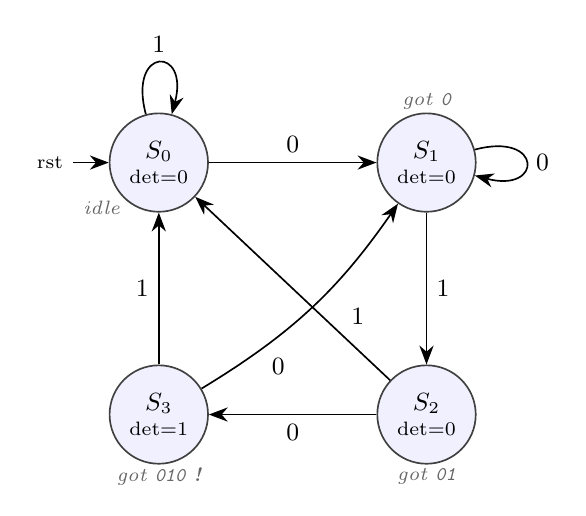
\begin{tikzpicture}[fsm,scale=1.00,transform shape]
\node[state,initial,label={[meaning]below left:{\textit{idle}}}] (S0) at (0.00,0.00) {$S_{0}$\\[-2pt]{\scriptsize det=0}};
\node[state,label={[meaning]above:{got \texttt{0}}}] (S1) at (3.40,0.00) {$S_{1}$\\[-2pt]{\scriptsize det=0}};
\node[state,label={[meaning]below:{got \texttt{01}}}] (S2) at (3.40,-3.20) {$S_{2}$\\[-2pt]{\scriptsize det=0}};
\node[state,label={[meaning]below:{got \texttt{010} \textbf{!}}}] (S3) at (0.00,-3.20) {$S_{3}$\\[-2pt]{\scriptsize det=1}};
\path (S0) edge[loop above] node[elab] {1} (S0);
\path (S0) edge[] node[elab] {0} (S1);
\path (S1) edge[loop right] node[elab] {0} (S1);
\path (S1) edge[] node[elab] {1} (S2);
\path (S2) edge[] node[elab] {0} (S3);
\path (S2) edge[] node[elab,pos=0.25,swap] {1} (S0);
\path (S3) edge[bend right=12] node[elab,pos=0.25,swap] {0} (S1);
\path (S3) edge[] node[elab] {1} (S0);
\end{tikzpicture}
\end{center}

\subsection{Step-by-step: watch the machine run on \texttt{101010010011}}
{\small Legend for the step-by-step pictures: \tikz\node[draw=black!75,fill=yellow!75,circle,minimum size=3mm,inner sep=0]{};~present state \quad \tikz\node[draw=red!80!black,line width=1.6pt,fill=blue!6,circle,minimum size=3mm,inner sep=0]{};~next state \quad \tikz\draw[->,>=Stealth,red!80!black,line width=1.6pt](0,0)--(0.6,0);~transition taken on this clock edge}\par\smallskip\noindent
\begin{minipage}[t]{0.327\textwidth}\centering
\fcolorbox{black!15}{white}{\begin{minipage}{0.94\linewidth}\centering
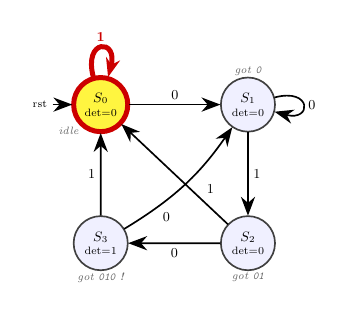
\begin{tikzpicture}[fsm,scale=0.55,transform shape]
\node[state,initial,cur,nxt,label={[meaning]below left:{\textit{idle}}}] (S0) at (0.00,0.00) {$S_{0}$\\[-2pt]{\scriptsize det=0}};
\node[state,label={[meaning]above:{got \texttt{0}}}] (S1) at (3.40,0.00) {$S_{1}$\\[-2pt]{\scriptsize det=0}};
\node[state,label={[meaning]below:{got \texttt{01}}}] (S2) at (3.40,-3.20) {$S_{2}$\\[-2pt]{\scriptsize det=0}};
\node[state,label={[meaning]below:{got \texttt{010} \textbf{!}}}] (S3) at (0.00,-3.20) {$S_{3}$\\[-2pt]{\scriptsize det=1}};
\path (S0) edge[loop above,hl] node[elab,hlnode] {1} (S0);
\path (S0) edge[] node[elab] {0} (S1);
\path (S1) edge[loop right] node[elab] {0} (S1);
\path (S1) edge[] node[elab] {1} (S2);
\path (S2) edge[] node[elab] {0} (S3);
\path (S2) edge[] node[elab,pos=0.25,swap] {1} (S0);
\path (S3) edge[bend right=12] node[elab,pos=0.25,swap] {0} (S1);
\path (S3) edge[] node[elab] {1} (S0);
\end{tikzpicture}
\\[2pt]{\small\textbf{Clock 1}: \texttt{serin=1}}\\[1pt]{\scriptsize $S_{0}$ $\rightarrow$ $S_{0}$ \;|\; det\_out=0 {\tiny(after edge)}}\end{minipage}}\end{minipage}
\hfill
\begin{minipage}[t]{0.327\textwidth}\centering
\fcolorbox{black!15}{white}{\begin{minipage}{0.94\linewidth}\centering
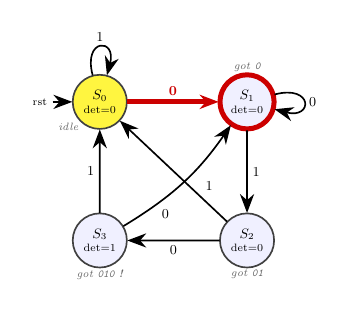
\begin{tikzpicture}[fsm,scale=0.55,transform shape]
\node[state,initial,cur,label={[meaning]below left:{\textit{idle}}}] (S0) at (0.00,0.00) {$S_{0}$\\[-2pt]{\scriptsize det=0}};
\node[state,nxt,label={[meaning]above:{got \texttt{0}}}] (S1) at (3.40,0.00) {$S_{1}$\\[-2pt]{\scriptsize det=0}};
\node[state,label={[meaning]below:{got \texttt{01}}}] (S2) at (3.40,-3.20) {$S_{2}$\\[-2pt]{\scriptsize det=0}};
\node[state,label={[meaning]below:{got \texttt{010} \textbf{!}}}] (S3) at (0.00,-3.20) {$S_{3}$\\[-2pt]{\scriptsize det=1}};
\path (S0) edge[loop above] node[elab] {1} (S0);
\path (S0) edge[hl] node[elab,hlnode] {0} (S1);
\path (S1) edge[loop right] node[elab] {0} (S1);
\path (S1) edge[] node[elab] {1} (S2);
\path (S2) edge[] node[elab] {0} (S3);
\path (S2) edge[] node[elab,pos=0.25,swap] {1} (S0);
\path (S3) edge[bend right=12] node[elab,pos=0.25,swap] {0} (S1);
\path (S3) edge[] node[elab] {1} (S0);
\end{tikzpicture}
\\[2pt]{\small\textbf{Clock 2}: \texttt{serin=0}}\\[1pt]{\scriptsize $S_{0}$ $\rightarrow$ $S_{1}$ \;|\; det\_out=0 {\tiny(after edge)}}\end{minipage}}\end{minipage}
\hfill
\begin{minipage}[t]{0.327\textwidth}\centering
\fcolorbox{black!15}{white}{\begin{minipage}{0.94\linewidth}\centering
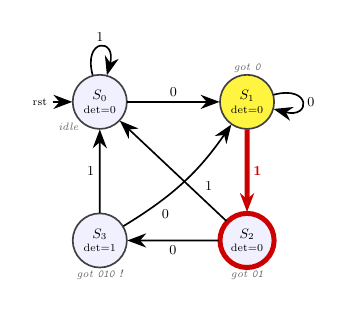
\begin{tikzpicture}[fsm,scale=0.55,transform shape]
\node[state,initial,label={[meaning]below left:{\textit{idle}}}] (S0) at (0.00,0.00) {$S_{0}$\\[-2pt]{\scriptsize det=0}};
\node[state,cur,label={[meaning]above:{got \texttt{0}}}] (S1) at (3.40,0.00) {$S_{1}$\\[-2pt]{\scriptsize det=0}};
\node[state,nxt,label={[meaning]below:{got \texttt{01}}}] (S2) at (3.40,-3.20) {$S_{2}$\\[-2pt]{\scriptsize det=0}};
\node[state,label={[meaning]below:{got \texttt{010} \textbf{!}}}] (S3) at (0.00,-3.20) {$S_{3}$\\[-2pt]{\scriptsize det=1}};
\path (S0) edge[loop above] node[elab] {1} (S0);
\path (S0) edge[] node[elab] {0} (S1);
\path (S1) edge[loop right] node[elab] {0} (S1);
\path (S1) edge[hl] node[elab,hlnode] {1} (S2);
\path (S2) edge[] node[elab] {0} (S3);
\path (S2) edge[] node[elab,pos=0.25,swap] {1} (S0);
\path (S3) edge[bend right=12] node[elab,pos=0.25,swap] {0} (S1);
\path (S3) edge[] node[elab] {1} (S0);
\end{tikzpicture}
\\[2pt]{\small\textbf{Clock 3}: \texttt{serin=1}}\\[1pt]{\scriptsize $S_{1}$ $\rightarrow$ $S_{2}$ \;|\; det\_out=0 {\tiny(after edge)}}\end{minipage}}\end{minipage}
\par\medskip\noindent
\begin{minipage}[t]{0.327\textwidth}\centering
\fcolorbox{black!15}{white}{\begin{minipage}{0.94\linewidth}\centering
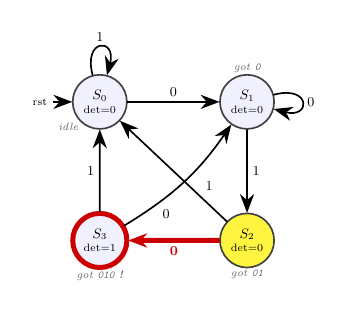
\begin{tikzpicture}[fsm,scale=0.55,transform shape]
\node[state,initial,label={[meaning]below left:{\textit{idle}}}] (S0) at (0.00,0.00) {$S_{0}$\\[-2pt]{\scriptsize det=0}};
\node[state,label={[meaning]above:{got \texttt{0}}}] (S1) at (3.40,0.00) {$S_{1}$\\[-2pt]{\scriptsize det=0}};
\node[state,cur,label={[meaning]below:{got \texttt{01}}}] (S2) at (3.40,-3.20) {$S_{2}$\\[-2pt]{\scriptsize det=0}};
\node[state,nxt,label={[meaning]below:{got \texttt{010} \textbf{!}}}] (S3) at (0.00,-3.20) {$S_{3}$\\[-2pt]{\scriptsize det=1}};
\path (S0) edge[loop above] node[elab] {1} (S0);
\path (S0) edge[] node[elab] {0} (S1);
\path (S1) edge[loop right] node[elab] {0} (S1);
\path (S1) edge[] node[elab] {1} (S2);
\path (S2) edge[hl] node[elab,hlnode] {0} (S3);
\path (S2) edge[] node[elab,pos=0.25,swap] {1} (S0);
\path (S3) edge[bend right=12] node[elab,pos=0.25,swap] {0} (S1);
\path (S3) edge[] node[elab] {1} (S0);
\end{tikzpicture}
\\[2pt]{\small\textbf{Clock 4}: \texttt{serin=0}}\\[1pt]{\scriptsize $S_{2}$ $\rightarrow$ $S_{3}$ \;|\; \textcolor{red!80!black}{\textbf{det\_out=1}} {\tiny(after edge)}}\end{minipage}}\end{minipage}
\hfill
\begin{minipage}[t]{0.327\textwidth}\centering
\fcolorbox{black!15}{white}{\begin{minipage}{0.94\linewidth}\centering
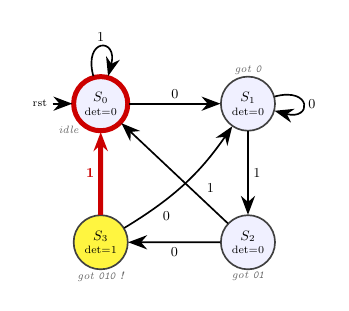
\begin{tikzpicture}[fsm,scale=0.55,transform shape]
\node[state,initial,nxt,label={[meaning]below left:{\textit{idle}}}] (S0) at (0.00,0.00) {$S_{0}$\\[-2pt]{\scriptsize det=0}};
\node[state,label={[meaning]above:{got \texttt{0}}}] (S1) at (3.40,0.00) {$S_{1}$\\[-2pt]{\scriptsize det=0}};
\node[state,label={[meaning]below:{got \texttt{01}}}] (S2) at (3.40,-3.20) {$S_{2}$\\[-2pt]{\scriptsize det=0}};
\node[state,cur,label={[meaning]below:{got \texttt{010} \textbf{!}}}] (S3) at (0.00,-3.20) {$S_{3}$\\[-2pt]{\scriptsize det=1}};
\path (S0) edge[loop above] node[elab] {1} (S0);
\path (S0) edge[] node[elab] {0} (S1);
\path (S1) edge[loop right] node[elab] {0} (S1);
\path (S1) edge[] node[elab] {1} (S2);
\path (S2) edge[] node[elab] {0} (S3);
\path (S2) edge[] node[elab,pos=0.25,swap] {1} (S0);
\path (S3) edge[bend right=12] node[elab,pos=0.25,swap] {0} (S1);
\path (S3) edge[hl] node[elab,hlnode] {1} (S0);
\end{tikzpicture}
\\[2pt]{\small\textbf{Clock 5}: \texttt{serin=1}}\\[1pt]{\scriptsize $S_{3}$ $\rightarrow$ $S_{0}$ \;|\; det\_out=0 {\tiny(after edge)}}\end{minipage}}\end{minipage}
\hfill
\begin{minipage}[t]{0.327\textwidth}\centering
\fcolorbox{black!15}{white}{\begin{minipage}{0.94\linewidth}\centering
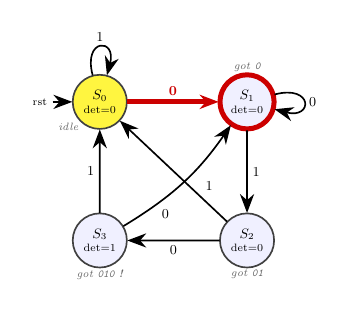
\begin{tikzpicture}[fsm,scale=0.55,transform shape]
\node[state,initial,cur,label={[meaning]below left:{\textit{idle}}}] (S0) at (0.00,0.00) {$S_{0}$\\[-2pt]{\scriptsize det=0}};
\node[state,nxt,label={[meaning]above:{got \texttt{0}}}] (S1) at (3.40,0.00) {$S_{1}$\\[-2pt]{\scriptsize det=0}};
\node[state,label={[meaning]below:{got \texttt{01}}}] (S2) at (3.40,-3.20) {$S_{2}$\\[-2pt]{\scriptsize det=0}};
\node[state,label={[meaning]below:{got \texttt{010} \textbf{!}}}] (S3) at (0.00,-3.20) {$S_{3}$\\[-2pt]{\scriptsize det=1}};
\path (S0) edge[loop above] node[elab] {1} (S0);
\path (S0) edge[hl] node[elab,hlnode] {0} (S1);
\path (S1) edge[loop right] node[elab] {0} (S1);
\path (S1) edge[] node[elab] {1} (S2);
\path (S2) edge[] node[elab] {0} (S3);
\path (S2) edge[] node[elab,pos=0.25,swap] {1} (S0);
\path (S3) edge[bend right=12] node[elab,pos=0.25,swap] {0} (S1);
\path (S3) edge[] node[elab] {1} (S0);
\end{tikzpicture}
\\[2pt]{\small\textbf{Clock 6}: \texttt{serin=0}}\\[1pt]{\scriptsize $S_{0}$ $\rightarrow$ $S_{1}$ \;|\; det\_out=0 {\tiny(after edge)}}\end{minipage}}\end{minipage}
\par\medskip\noindent
\begin{minipage}[t]{0.327\textwidth}\centering
\fcolorbox{black!15}{white}{\begin{minipage}{0.94\linewidth}\centering
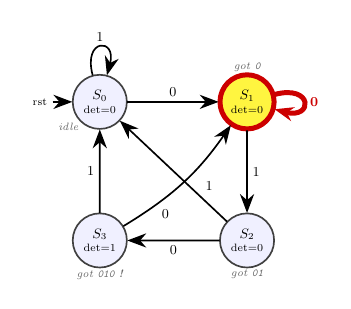
\begin{tikzpicture}[fsm,scale=0.55,transform shape]
\node[state,initial,label={[meaning]below left:{\textit{idle}}}] (S0) at (0.00,0.00) {$S_{0}$\\[-2pt]{\scriptsize det=0}};
\node[state,cur,nxt,label={[meaning]above:{got \texttt{0}}}] (S1) at (3.40,0.00) {$S_{1}$\\[-2pt]{\scriptsize det=0}};
\node[state,label={[meaning]below:{got \texttt{01}}}] (S2) at (3.40,-3.20) {$S_{2}$\\[-2pt]{\scriptsize det=0}};
\node[state,label={[meaning]below:{got \texttt{010} \textbf{!}}}] (S3) at (0.00,-3.20) {$S_{3}$\\[-2pt]{\scriptsize det=1}};
\path (S0) edge[loop above] node[elab] {1} (S0);
\path (S0) edge[] node[elab] {0} (S1);
\path (S1) edge[loop right,hl] node[elab,hlnode] {0} (S1);
\path (S1) edge[] node[elab] {1} (S2);
\path (S2) edge[] node[elab] {0} (S3);
\path (S2) edge[] node[elab,pos=0.25,swap] {1} (S0);
\path (S3) edge[bend right=12] node[elab,pos=0.25,swap] {0} (S1);
\path (S3) edge[] node[elab] {1} (S0);
\end{tikzpicture}
\\[2pt]{\small\textbf{Clock 7}: \texttt{serin=0}}\\[1pt]{\scriptsize $S_{1}$ $\rightarrow$ $S_{1}$ \;|\; det\_out=0 {\tiny(after edge)}}\end{minipage}}\end{minipage}
\hfill
\begin{minipage}[t]{0.327\textwidth}\centering
\fcolorbox{black!15}{white}{\begin{minipage}{0.94\linewidth}\centering
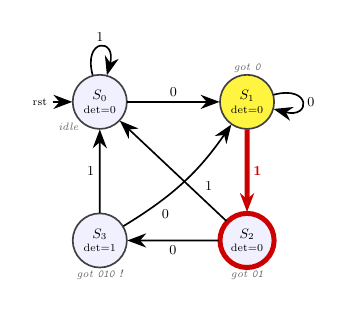
\begin{tikzpicture}[fsm,scale=0.55,transform shape]
\node[state,initial,label={[meaning]below left:{\textit{idle}}}] (S0) at (0.00,0.00) {$S_{0}$\\[-2pt]{\scriptsize det=0}};
\node[state,cur,label={[meaning]above:{got \texttt{0}}}] (S1) at (3.40,0.00) {$S_{1}$\\[-2pt]{\scriptsize det=0}};
\node[state,nxt,label={[meaning]below:{got \texttt{01}}}] (S2) at (3.40,-3.20) {$S_{2}$\\[-2pt]{\scriptsize det=0}};
\node[state,label={[meaning]below:{got \texttt{010} \textbf{!}}}] (S3) at (0.00,-3.20) {$S_{3}$\\[-2pt]{\scriptsize det=1}};
\path (S0) edge[loop above] node[elab] {1} (S0);
\path (S0) edge[] node[elab] {0} (S1);
\path (S1) edge[loop right] node[elab] {0} (S1);
\path (S1) edge[hl] node[elab,hlnode] {1} (S2);
\path (S2) edge[] node[elab] {0} (S3);
\path (S2) edge[] node[elab,pos=0.25,swap] {1} (S0);
\path (S3) edge[bend right=12] node[elab,pos=0.25,swap] {0} (S1);
\path (S3) edge[] node[elab] {1} (S0);
\end{tikzpicture}
\\[2pt]{\small\textbf{Clock 8}: \texttt{serin=1}}\\[1pt]{\scriptsize $S_{1}$ $\rightarrow$ $S_{2}$ \;|\; det\_out=0 {\tiny(after edge)}}\end{minipage}}\end{minipage}
\hfill
\begin{minipage}[t]{0.327\textwidth}\centering
\fcolorbox{black!15}{white}{\begin{minipage}{0.94\linewidth}\centering
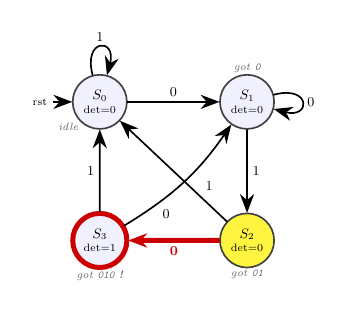
\begin{tikzpicture}[fsm,scale=0.55,transform shape]
\node[state,initial,label={[meaning]below left:{\textit{idle}}}] (S0) at (0.00,0.00) {$S_{0}$\\[-2pt]{\scriptsize det=0}};
\node[state,label={[meaning]above:{got \texttt{0}}}] (S1) at (3.40,0.00) {$S_{1}$\\[-2pt]{\scriptsize det=0}};
\node[state,cur,label={[meaning]below:{got \texttt{01}}}] (S2) at (3.40,-3.20) {$S_{2}$\\[-2pt]{\scriptsize det=0}};
\node[state,nxt,label={[meaning]below:{got \texttt{010} \textbf{!}}}] (S3) at (0.00,-3.20) {$S_{3}$\\[-2pt]{\scriptsize det=1}};
\path (S0) edge[loop above] node[elab] {1} (S0);
\path (S0) edge[] node[elab] {0} (S1);
\path (S1) edge[loop right] node[elab] {0} (S1);
\path (S1) edge[] node[elab] {1} (S2);
\path (S2) edge[hl] node[elab,hlnode] {0} (S3);
\path (S2) edge[] node[elab,pos=0.25,swap] {1} (S0);
\path (S3) edge[bend right=12] node[elab,pos=0.25,swap] {0} (S1);
\path (S3) edge[] node[elab] {1} (S0);
\end{tikzpicture}
\\[2pt]{\small\textbf{Clock 9}: \texttt{serin=0}}\\[1pt]{\scriptsize $S_{2}$ $\rightarrow$ $S_{3}$ \;|\; \textcolor{red!80!black}{\textbf{det\_out=1}} {\tiny(after edge)}}\end{minipage}}\end{minipage}
\par\medskip\noindent
\begin{minipage}[t]{0.327\textwidth}\centering
\fcolorbox{black!15}{white}{\begin{minipage}{0.94\linewidth}\centering
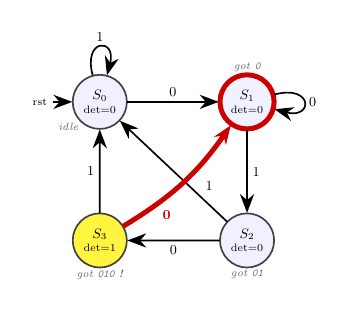
\begin{tikzpicture}[fsm,scale=0.55,transform shape]
\node[state,initial,label={[meaning]below left:{\textit{idle}}}] (S0) at (0.00,0.00) {$S_{0}$\\[-2pt]{\scriptsize det=0}};
\node[state,nxt,label={[meaning]above:{got \texttt{0}}}] (S1) at (3.40,0.00) {$S_{1}$\\[-2pt]{\scriptsize det=0}};
\node[state,label={[meaning]below:{got \texttt{01}}}] (S2) at (3.40,-3.20) {$S_{2}$\\[-2pt]{\scriptsize det=0}};
\node[state,cur,label={[meaning]below:{got \texttt{010} \textbf{!}}}] (S3) at (0.00,-3.20) {$S_{3}$\\[-2pt]{\scriptsize det=1}};
\path (S0) edge[loop above] node[elab] {1} (S0);
\path (S0) edge[] node[elab] {0} (S1);
\path (S1) edge[loop right] node[elab] {0} (S1);
\path (S1) edge[] node[elab] {1} (S2);
\path (S2) edge[] node[elab] {0} (S3);
\path (S2) edge[] node[elab,pos=0.25,swap] {1} (S0);
\path (S3) edge[bend right=12,hl] node[elab,pos=0.25,swap,hlnode] {0} (S1);
\path (S3) edge[] node[elab] {1} (S0);
\end{tikzpicture}
\\[2pt]{\small\textbf{Clock 10}: \texttt{serin=0}}\\[1pt]{\scriptsize $S_{3}$ $\rightarrow$ $S_{1}$ \;|\; det\_out=0 {\tiny(after edge)}}\end{minipage}}\end{minipage}
\hfill
\begin{minipage}[t]{0.327\textwidth}\centering
\fcolorbox{black!15}{white}{\begin{minipage}{0.94\linewidth}\centering
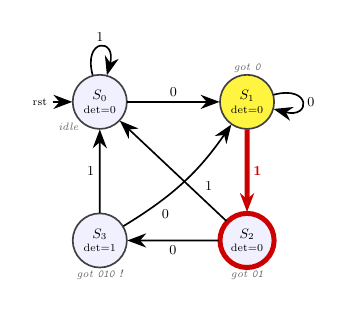
\begin{tikzpicture}[fsm,scale=0.55,transform shape]
\node[state,initial,label={[meaning]below left:{\textit{idle}}}] (S0) at (0.00,0.00) {$S_{0}$\\[-2pt]{\scriptsize det=0}};
\node[state,cur,label={[meaning]above:{got \texttt{0}}}] (S1) at (3.40,0.00) {$S_{1}$\\[-2pt]{\scriptsize det=0}};
\node[state,nxt,label={[meaning]below:{got \texttt{01}}}] (S2) at (3.40,-3.20) {$S_{2}$\\[-2pt]{\scriptsize det=0}};
\node[state,label={[meaning]below:{got \texttt{010} \textbf{!}}}] (S3) at (0.00,-3.20) {$S_{3}$\\[-2pt]{\scriptsize det=1}};
\path (S0) edge[loop above] node[elab] {1} (S0);
\path (S0) edge[] node[elab] {0} (S1);
\path (S1) edge[loop right] node[elab] {0} (S1);
\path (S1) edge[hl] node[elab,hlnode] {1} (S2);
\path (S2) edge[] node[elab] {0} (S3);
\path (S2) edge[] node[elab,pos=0.25,swap] {1} (S0);
\path (S3) edge[bend right=12] node[elab,pos=0.25,swap] {0} (S1);
\path (S3) edge[] node[elab] {1} (S0);
\end{tikzpicture}
\\[2pt]{\small\textbf{Clock 11}: \texttt{serin=1}}\\[1pt]{\scriptsize $S_{1}$ $\rightarrow$ $S_{2}$ \;|\; det\_out=0 {\tiny(after edge)}}\end{minipage}}\end{minipage}
\hfill
\begin{minipage}[t]{0.327\textwidth}\centering
\fcolorbox{black!15}{white}{\begin{minipage}{0.94\linewidth}\centering
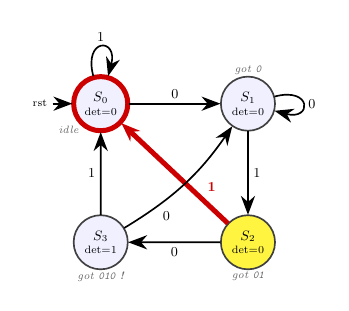
\begin{tikzpicture}[fsm,scale=0.55,transform shape]
\node[state,initial,nxt,label={[meaning]below left:{\textit{idle}}}] (S0) at (0.00,0.00) {$S_{0}$\\[-2pt]{\scriptsize det=0}};
\node[state,label={[meaning]above:{got \texttt{0}}}] (S1) at (3.40,0.00) {$S_{1}$\\[-2pt]{\scriptsize det=0}};
\node[state,cur,label={[meaning]below:{got \texttt{01}}}] (S2) at (3.40,-3.20) {$S_{2}$\\[-2pt]{\scriptsize det=0}};
\node[state,label={[meaning]below:{got \texttt{010} \textbf{!}}}] (S3) at (0.00,-3.20) {$S_{3}$\\[-2pt]{\scriptsize det=1}};
\path (S0) edge[loop above] node[elab] {1} (S0);
\path (S0) edge[] node[elab] {0} (S1);
\path (S1) edge[loop right] node[elab] {0} (S1);
\path (S1) edge[] node[elab] {1} (S2);
\path (S2) edge[] node[elab] {0} (S3);
\path (S2) edge[hl] node[elab,pos=0.25,swap,hlnode] {1} (S0);
\path (S3) edge[bend right=12] node[elab,pos=0.25,swap] {0} (S1);
\path (S3) edge[] node[elab] {1} (S0);
\end{tikzpicture}
\\[2pt]{\small\textbf{Clock 12}: \texttt{serin=1}}\\[1pt]{\scriptsize $S_{2}$ $\rightarrow$ $S_{0}$ \;|\; det\_out=0 {\tiny(after edge)}}\end{minipage}}\end{minipage}
\par\medskip\noindent

\begin{tip}[Notice the non-overlap at clocks 2--6]
The input \texttt{01010} (clocks 2--6) contains ``010'' at clocks 2--4 \emph{and} ``010'' at clocks 4--6,
sharing the 0 of clock 4. Non-overlapping counts only the first one. At clock 5 the 1 sends
$S_3\to S_0$, so the shared 0 is not reused, and the next detection needs a brand-new ``010''.
\end{tip}

\subsection{Trace table}
\begin{center}\small
\begin{tabular}{c c c c c}
\toprule
Clock edge & \texttt{serin} sampled & Present state & Next state & \texttt{det\_out} {\scriptsize after edge (Moore)}\\
\midrule
1 & \texttt{1} & $S_{0}$ & $S_{0}$ & 0\\
2 & \texttt{0} & $S_{0}$ & $S_{1}$ & 0\\
3 & \texttt{1} & $S_{1}$ & $S_{2}$ & 0\\
\rowcolor{red!12}4 & \texttt{0} & $S_{2}$ & $S_{3}$ & \textbf{1}\\
5 & \texttt{1} & $S_{3}$ & $S_{0}$ & 0\\
6 & \texttt{0} & $S_{0}$ & $S_{1}$ & 0\\
7 & \texttt{0} & $S_{1}$ & $S_{1}$ & 0\\
8 & \texttt{1} & $S_{1}$ & $S_{2}$ & 0\\
\rowcolor{red!12}9 & \texttt{0} & $S_{2}$ & $S_{3}$ & \textbf{1}\\
10 & \texttt{0} & $S_{3}$ & $S_{1}$ & 0\\
11 & \texttt{1} & $S_{1}$ & $S_{2}$ & 0\\
12 & \texttt{1} & $S_{2}$ & $S_{0}$ & 0\\
13 & \texttt{0} & $S_{0}$ & $S_{1}$ & 0\\
14 & \texttt{1} & $S_{1}$ & $S_{2}$ & 0\\
\rowcolor{red!12}15 & \texttt{0} & $S_{2}$ & $S_{3}$ & \textbf{1}\\
16 & \texttt{1} & $S_{3}$ & $S_{0}$ & 0\\
17 & \texttt{0} & $S_{0}$ & $S_{1}$ & 0\\
18 & \texttt{0} & $S_{1}$ & $S_{1}$ & 0\\
19 & \texttt{1} & $S_{1}$ & $S_{2}$ & 0\\
20 & \texttt{1} & $S_{2}$ & $S_{0}$ & 0\\
\bottomrule
\end{tabular}\end{center}

\subsection{Waveform (Moore and Mealy versions on the same input)}
\begin{center}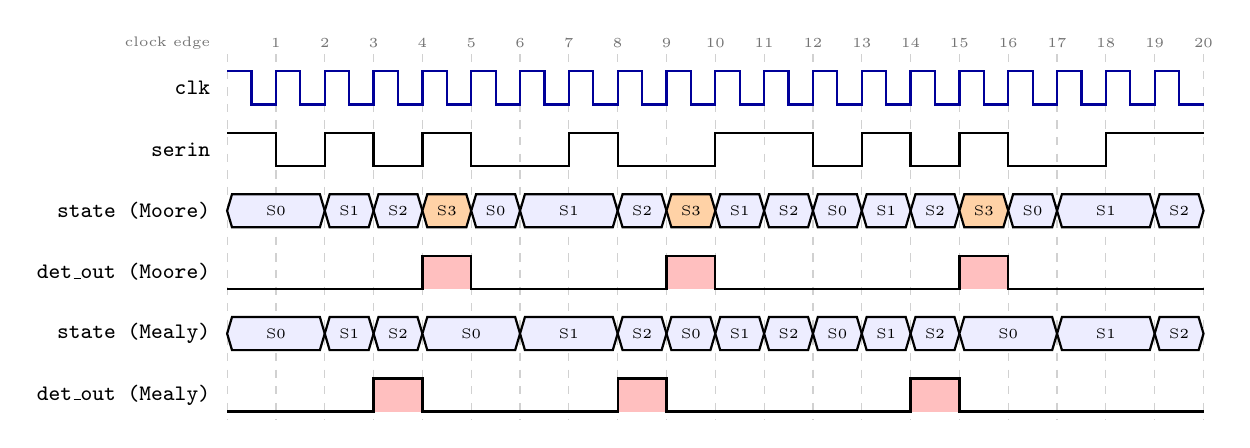
\begin{tikzpicture}[x=0.62cm,y=1cm,font=\scriptsize]
\draw[black!18,dashed] (0,0.64)--(0,-4.00);
\draw[black!18,dashed] (1,0.64)--(1,-4.00);
\node[black!55,font=\tiny] at (1,0.78) {1};
\draw[black!18,dashed] (2,0.64)--(2,-4.00);
\node[black!55,font=\tiny] at (2,0.78) {2};
\draw[black!18,dashed] (3,0.64)--(3,-4.00);
\node[black!55,font=\tiny] at (3,0.78) {3};
\draw[black!18,dashed] (4,0.64)--(4,-4.00);
\node[black!55,font=\tiny] at (4,0.78) {4};
\draw[black!18,dashed] (5,0.64)--(5,-4.00);
\node[black!55,font=\tiny] at (5,0.78) {5};
\draw[black!18,dashed] (6,0.64)--(6,-4.00);
\node[black!55,font=\tiny] at (6,0.78) {6};
\draw[black!18,dashed] (7,0.64)--(7,-4.00);
\node[black!55,font=\tiny] at (7,0.78) {7};
\draw[black!18,dashed] (8,0.64)--(8,-4.00);
\node[black!55,font=\tiny] at (8,0.78) {8};
\draw[black!18,dashed] (9,0.64)--(9,-4.00);
\node[black!55,font=\tiny] at (9,0.78) {9};
\draw[black!18,dashed] (10,0.64)--(10,-4.00);
\node[black!55,font=\tiny] at (10,0.78) {10};
\draw[black!18,dashed] (11,0.64)--(11,-4.00);
\node[black!55,font=\tiny] at (11,0.78) {11};
\draw[black!18,dashed] (12,0.64)--(12,-4.00);
\node[black!55,font=\tiny] at (12,0.78) {12};
\draw[black!18,dashed] (13,0.64)--(13,-4.00);
\node[black!55,font=\tiny] at (13,0.78) {13};
\draw[black!18,dashed] (14,0.64)--(14,-4.00);
\node[black!55,font=\tiny] at (14,0.78) {14};
\draw[black!18,dashed] (15,0.64)--(15,-4.00);
\node[black!55,font=\tiny] at (15,0.78) {15};
\draw[black!18,dashed] (16,0.64)--(16,-4.00);
\node[black!55,font=\tiny] at (16,0.78) {16};
\draw[black!18,dashed] (17,0.64)--(17,-4.00);
\node[black!55,font=\tiny] at (17,0.78) {17};
\draw[black!18,dashed] (18,0.64)--(18,-4.00);
\node[black!55,font=\tiny] at (18,0.78) {18};
\draw[black!18,dashed] (19,0.64)--(19,-4.00);
\node[black!55,font=\tiny] at (19,0.78) {19};
\draw[black!18,dashed] (20,0.64)--(20,-4.00);
\node[black!55,font=\tiny] at (20,0.78) {20};
\node[anchor=east,black!55,font=\tiny] at (-0.15,0.78) {clock edge};
\node[anchor=east,font=\footnotesize\ttfamily] at (-0.15,0.21) {clk};
\draw[thick,blue!60!black] (0.000,0.420) -- (0.500,0.420) -- (0.500,0.000) -- (1.000,0.000) -- (1.000,0.420) -- (1.500,0.420) -- (1.500,0.000) -- (2.000,0.000) -- (2.000,0.420) -- (2.500,0.420) -- (2.500,0.000) -- (3.000,0.000) -- (3.000,0.420) -- (3.500,0.420) -- (3.500,0.000) -- (4.000,0.000) -- (4.000,0.420) -- (4.500,0.420) -- (4.500,0.000) -- (5.000,0.000) -- (5.000,0.420) -- (5.500,0.420) -- (5.500,0.000) -- (6.000,0.000) -- (6.000,0.420) -- (6.500,0.420) -- (6.500,0.000) -- (7.000,0.000) -- (7.000,0.420) -- (7.500,0.420) -- (7.500,0.000) -- (8.000,0.000) -- (8.000,0.420) -- (8.500,0.420) -- (8.500,0.000) -- (9.000,0.000) -- (9.000,0.420) -- (9.500,0.420) -- (9.500,0.000) -- (10.000,0.000) -- (10.000,0.420) -- (10.500,0.420) -- (10.500,0.000) -- (11.000,0.000) -- (11.000,0.420) -- (11.500,0.420) -- (11.500,0.000) -- (12.000,0.000) -- (12.000,0.420) -- (12.500,0.420) -- (12.500,0.000) -- (13.000,0.000) -- (13.000,0.420) -- (13.500,0.420) -- (13.500,0.000) -- (14.000,0.000) -- (14.000,0.420) -- (14.500,0.420) -- (14.500,0.000) -- (15.000,0.000) -- (15.000,0.420) -- (15.500,0.420) -- (15.500,0.000) -- (16.000,0.000) -- (16.000,0.420) -- (16.500,0.420) -- (16.500,0.000) -- (17.000,0.000) -- (17.000,0.420) -- (17.500,0.420) -- (17.500,0.000) -- (18.000,0.000) -- (18.000,0.420) -- (18.500,0.420) -- (18.500,0.000) -- (19.000,0.000) -- (19.000,0.420) -- (19.500,0.420) -- (19.500,0.000) -- (20.000,0.000);
\node[anchor=east,font=\footnotesize\ttfamily] at (-0.15,-0.57) {serin};
\draw[thick,black] (0.000,-0.360) -- (1.000,-0.360) -- (1.000,-0.780) -- (2.000,-0.780) -- (2.000,-0.360) -- (3.000,-0.360) -- (3.000,-0.780) -- (4.000,-0.780) -- (4.000,-0.360) -- (5.000,-0.360) -- (5.000,-0.780) -- (6.000,-0.780) -- (6.000,-0.780) -- (7.000,-0.780) -- (7.000,-0.360) -- (8.000,-0.360) -- (8.000,-0.780) -- (9.000,-0.780) -- (9.000,-0.780) -- (10.000,-0.780) -- (10.000,-0.360) -- (11.000,-0.360) -- (11.000,-0.360) -- (12.000,-0.360) -- (12.000,-0.780) -- (13.000,-0.780) -- (13.000,-0.360) -- (14.000,-0.360) -- (14.000,-0.780) -- (15.000,-0.780) -- (15.000,-0.360) -- (16.000,-0.360) -- (16.000,-0.780) -- (17.000,-0.780) -- (17.000,-0.780) -- (18.000,-0.780) -- (18.000,-0.360) -- (19.000,-0.360) -- (19.000,-0.360) -- (20.000,-0.360);
\node[anchor=east,font=\footnotesize\ttfamily] at (-0.15,-1.35) {state (Moore)};
\draw[thick,fill=blue!7] (0.000,-1.350)--(0.100,-1.140)--(1.900,-1.140)--(2.000,-1.350)--(1.900,-1.560)--(0.100,-1.560)--cycle;
\node[font=\tiny] at (1.000,-1.350) {S0};
\draw[thick,fill=blue!7] (2.000,-1.350)--(2.100,-1.140)--(2.900,-1.140)--(3.000,-1.350)--(2.900,-1.560)--(2.100,-1.560)--cycle;
\node[font=\tiny] at (2.500,-1.350) {S1};
\draw[thick,fill=blue!7] (3.000,-1.350)--(3.100,-1.140)--(3.900,-1.140)--(4.000,-1.350)--(3.900,-1.560)--(3.100,-1.560)--cycle;
\node[font=\tiny] at (3.500,-1.350) {S2};
\draw[thick,fill=orange!35] (4.000,-1.350)--(4.100,-1.140)--(4.900,-1.140)--(5.000,-1.350)--(4.900,-1.560)--(4.100,-1.560)--cycle;
\node[font=\tiny] at (4.500,-1.350) {S3};
\draw[thick,fill=blue!7] (5.000,-1.350)--(5.100,-1.140)--(5.900,-1.140)--(6.000,-1.350)--(5.900,-1.560)--(5.100,-1.560)--cycle;
\node[font=\tiny] at (5.500,-1.350) {S0};
\draw[thick,fill=blue!7] (6.000,-1.350)--(6.100,-1.140)--(7.900,-1.140)--(8.000,-1.350)--(7.900,-1.560)--(6.100,-1.560)--cycle;
\node[font=\tiny] at (7.000,-1.350) {S1};
\draw[thick,fill=blue!7] (8.000,-1.350)--(8.100,-1.140)--(8.900,-1.140)--(9.000,-1.350)--(8.900,-1.560)--(8.100,-1.560)--cycle;
\node[font=\tiny] at (8.500,-1.350) {S2};
\draw[thick,fill=orange!35] (9.000,-1.350)--(9.100,-1.140)--(9.900,-1.140)--(10.000,-1.350)--(9.900,-1.560)--(9.100,-1.560)--cycle;
\node[font=\tiny] at (9.500,-1.350) {S3};
\draw[thick,fill=blue!7] (10.000,-1.350)--(10.100,-1.140)--(10.900,-1.140)--(11.000,-1.350)--(10.900,-1.560)--(10.100,-1.560)--cycle;
\node[font=\tiny] at (10.500,-1.350) {S1};
\draw[thick,fill=blue!7] (11.000,-1.350)--(11.100,-1.140)--(11.900,-1.140)--(12.000,-1.350)--(11.900,-1.560)--(11.100,-1.560)--cycle;
\node[font=\tiny] at (11.500,-1.350) {S2};
\draw[thick,fill=blue!7] (12.000,-1.350)--(12.100,-1.140)--(12.900,-1.140)--(13.000,-1.350)--(12.900,-1.560)--(12.100,-1.560)--cycle;
\node[font=\tiny] at (12.500,-1.350) {S0};
\draw[thick,fill=blue!7] (13.000,-1.350)--(13.100,-1.140)--(13.900,-1.140)--(14.000,-1.350)--(13.900,-1.560)--(13.100,-1.560)--cycle;
\node[font=\tiny] at (13.500,-1.350) {S1};
\draw[thick,fill=blue!7] (14.000,-1.350)--(14.100,-1.140)--(14.900,-1.140)--(15.000,-1.350)--(14.900,-1.560)--(14.100,-1.560)--cycle;
\node[font=\tiny] at (14.500,-1.350) {S2};
\draw[thick,fill=orange!35] (15.000,-1.350)--(15.100,-1.140)--(15.900,-1.140)--(16.000,-1.350)--(15.900,-1.560)--(15.100,-1.560)--cycle;
\node[font=\tiny] at (15.500,-1.350) {S3};
\draw[thick,fill=blue!7] (16.000,-1.350)--(16.100,-1.140)--(16.900,-1.140)--(17.000,-1.350)--(16.900,-1.560)--(16.100,-1.560)--cycle;
\node[font=\tiny] at (16.500,-1.350) {S0};
\draw[thick,fill=blue!7] (17.000,-1.350)--(17.100,-1.140)--(18.900,-1.140)--(19.000,-1.350)--(18.900,-1.560)--(17.100,-1.560)--cycle;
\node[font=\tiny] at (18.000,-1.350) {S1};
\draw[thick,fill=blue!7] (19.000,-1.350)--(19.100,-1.140)--(19.900,-1.140)--(20.000,-1.350)--(19.900,-1.560)--(19.100,-1.560)--cycle;
\node[font=\tiny] at (19.500,-1.350) {S2};
\node[anchor=east,font=\footnotesize\ttfamily] at (-0.15,-2.13) {det\_out (Moore)};
\fill[red!25] (4.000,-2.340) rectangle (5.000,-1.920);
\fill[red!25] (9.000,-2.340) rectangle (10.000,-1.920);
\fill[red!25] (15.000,-2.340) rectangle (16.000,-1.920);
\draw[thick,black] (0.000,-2.340) -- (1.000,-2.340) -- (1.000,-2.340) -- (2.000,-2.340) -- (2.000,-2.340) -- (3.000,-2.340) -- (3.000,-2.340) -- (4.000,-2.340) -- (4.000,-1.920) -- (5.000,-1.920) -- (5.000,-2.340) -- (6.000,-2.340) -- (6.000,-2.340) -- (7.000,-2.340) -- (7.000,-2.340) -- (8.000,-2.340) -- (8.000,-2.340) -- (9.000,-2.340) -- (9.000,-1.920) -- (10.000,-1.920) -- (10.000,-2.340) -- (11.000,-2.340) -- (11.000,-2.340) -- (12.000,-2.340) -- (12.000,-2.340) -- (13.000,-2.340) -- (13.000,-2.340) -- (14.000,-2.340) -- (14.000,-2.340) -- (15.000,-2.340) -- (15.000,-1.920) -- (16.000,-1.920) -- (16.000,-2.340) -- (17.000,-2.340) -- (17.000,-2.340) -- (18.000,-2.340) -- (18.000,-2.340) -- (19.000,-2.340) -- (19.000,-2.340) -- (20.000,-2.340);
\node[anchor=east,font=\footnotesize\ttfamily] at (-0.15,-2.91) {state (Mealy)};
\draw[thick,fill=blue!7] (0.000,-2.910)--(0.100,-2.700)--(1.900,-2.700)--(2.000,-2.910)--(1.900,-3.120)--(0.100,-3.120)--cycle;
\node[font=\tiny] at (1.000,-2.910) {S0};
\draw[thick,fill=blue!7] (2.000,-2.910)--(2.100,-2.700)--(2.900,-2.700)--(3.000,-2.910)--(2.900,-3.120)--(2.100,-3.120)--cycle;
\node[font=\tiny] at (2.500,-2.910) {S1};
\draw[thick,fill=blue!7] (3.000,-2.910)--(3.100,-2.700)--(3.900,-2.700)--(4.000,-2.910)--(3.900,-3.120)--(3.100,-3.120)--cycle;
\node[font=\tiny] at (3.500,-2.910) {S2};
\draw[thick,fill=blue!7] (4.000,-2.910)--(4.100,-2.700)--(5.900,-2.700)--(6.000,-2.910)--(5.900,-3.120)--(4.100,-3.120)--cycle;
\node[font=\tiny] at (5.000,-2.910) {S0};
\draw[thick,fill=blue!7] (6.000,-2.910)--(6.100,-2.700)--(7.900,-2.700)--(8.000,-2.910)--(7.900,-3.120)--(6.100,-3.120)--cycle;
\node[font=\tiny] at (7.000,-2.910) {S1};
\draw[thick,fill=blue!7] (8.000,-2.910)--(8.100,-2.700)--(8.900,-2.700)--(9.000,-2.910)--(8.900,-3.120)--(8.100,-3.120)--cycle;
\node[font=\tiny] at (8.500,-2.910) {S2};
\draw[thick,fill=blue!7] (9.000,-2.910)--(9.100,-2.700)--(9.900,-2.700)--(10.000,-2.910)--(9.900,-3.120)--(9.100,-3.120)--cycle;
\node[font=\tiny] at (9.500,-2.910) {S0};
\draw[thick,fill=blue!7] (10.000,-2.910)--(10.100,-2.700)--(10.900,-2.700)--(11.000,-2.910)--(10.900,-3.120)--(10.100,-3.120)--cycle;
\node[font=\tiny] at (10.500,-2.910) {S1};
\draw[thick,fill=blue!7] (11.000,-2.910)--(11.100,-2.700)--(11.900,-2.700)--(12.000,-2.910)--(11.900,-3.120)--(11.100,-3.120)--cycle;
\node[font=\tiny] at (11.500,-2.910) {S2};
\draw[thick,fill=blue!7] (12.000,-2.910)--(12.100,-2.700)--(12.900,-2.700)--(13.000,-2.910)--(12.900,-3.120)--(12.100,-3.120)--cycle;
\node[font=\tiny] at (12.500,-2.910) {S0};
\draw[thick,fill=blue!7] (13.000,-2.910)--(13.100,-2.700)--(13.900,-2.700)--(14.000,-2.910)--(13.900,-3.120)--(13.100,-3.120)--cycle;
\node[font=\tiny] at (13.500,-2.910) {S1};
\draw[thick,fill=blue!7] (14.000,-2.910)--(14.100,-2.700)--(14.900,-2.700)--(15.000,-2.910)--(14.900,-3.120)--(14.100,-3.120)--cycle;
\node[font=\tiny] at (14.500,-2.910) {S2};
\draw[thick,fill=blue!7] (15.000,-2.910)--(15.100,-2.700)--(16.900,-2.700)--(17.000,-2.910)--(16.900,-3.120)--(15.100,-3.120)--cycle;
\node[font=\tiny] at (16.000,-2.910) {S0};
\draw[thick,fill=blue!7] (17.000,-2.910)--(17.100,-2.700)--(18.900,-2.700)--(19.000,-2.910)--(18.900,-3.120)--(17.100,-3.120)--cycle;
\node[font=\tiny] at (18.000,-2.910) {S1};
\draw[thick,fill=blue!7] (19.000,-2.910)--(19.100,-2.700)--(19.900,-2.700)--(20.000,-2.910)--(19.900,-3.120)--(19.100,-3.120)--cycle;
\node[font=\tiny] at (19.500,-2.910) {S2};
\node[anchor=east,font=\footnotesize\ttfamily] at (-0.15,-3.69) {det\_out (Mealy)};
\fill[red!25] (3.000,-3.900) rectangle (4.000,-3.480);
\fill[red!25] (8.000,-3.900) rectangle (9.000,-3.480);
\fill[red!25] (14.000,-3.900) rectangle (15.000,-3.480);
\draw[thick,black] (0.000,-3.900) -- (1.000,-3.900) -- (1.000,-3.900) -- (2.000,-3.900) -- (2.000,-3.900) -- (3.000,-3.900) -- (3.000,-3.480) -- (4.000,-3.480) -- (4.000,-3.900) -- (5.000,-3.900) -- (5.000,-3.900) -- (6.000,-3.900) -- (6.000,-3.900) -- (7.000,-3.900) -- (7.000,-3.900) -- (8.000,-3.900) -- (8.000,-3.480) -- (9.000,-3.480) -- (9.000,-3.900) -- (10.000,-3.900) -- (10.000,-3.900) -- (11.000,-3.900) -- (11.000,-3.900) -- (12.000,-3.900) -- (12.000,-3.900) -- (13.000,-3.900) -- (13.000,-3.900) -- (14.000,-3.900) -- (14.000,-3.480) -- (15.000,-3.480) -- (15.000,-3.900) -- (16.000,-3.900) -- (16.000,-3.900) -- (17.000,-3.900) -- (17.000,-3.900) -- (18.000,-3.900) -- (18.000,-3.900) -- (19.000,-3.900) -- (19.000,-3.900) -- (20.000,-3.900);
\end{tikzpicture}\end{center}
{\small Moore raises \texttt{det\_out} for the clock \emph{after} the edge that sampled the final 0.
Mealy raises it while that final 0 is still on the input, one clock earlier and with one state fewer.}

\subsection{RTL -- Moore version, slice by slice}
\begin{codeslice}{Slice 1 -- ports and state encoding}{seq010\_moore.v}
\slicenote{One state per ``how much of 010 have I seen''. Two bits are enough for four states.}
\begin{lstlisting}
`timescale 1ns/1ps
// Non-overlapping "010" sequence detector -- Moore FSM
module seq010_moore (
    input  wire clk,
    input  wire rst,       // active-high asynchronous reset
    input  wire serin,     // serial input, one bit per clock
    output reg  det_out    // high for one clock after "010" is seen
);
    localparam [1:0] S0 = 2'b00,   // idle (nothing useful yet)
                     S1 = 2'b01,   // got "0"
                     S2 = 2'b10,   // got "01"
                     S3 = 2'b11;   // got "010"  -> det_out = 1

    reg [1:0] state, next_state;
\end{lstlisting}
\end{codeslice}
\begin{codeslice}{Slice 2 -- state register (the only clocked block)}{seq010\_moore.v}
\slicenote{Non-blocking \texttt{<=}, reset to the idle state.}
\begin{lstlisting}
    // (1) state register
    always @(posedge clk or posedge rst) begin
        if (rst) state <= S0;
        else     state <= next_state;
    end
\end{lstlisting}
\end{codeslice}
\begin{codeslice}{Slice 3 -- next-state logic (combinational)}{seq010\_moore.v}
\slicenote{Blocking \texttt{=}, a default assignment so no latch is inferred, and one line per bubble of the diagram.}
\begin{lstlisting}
    // (2) next-state logic
    always @(*) begin
        next_state = S0;                          // default: no latch
        case (state)
            S0: next_state = (serin == 1'b0) ? S1 : S0;
            S1: next_state = (serin == 1'b1) ? S2 : S1;
            S2: next_state = (serin == 1'b0) ? S3 : S0;
            // NON-overlap: the "0" that completed 010 is NOT reused.
            // A new 0 starts a fresh sequence, a 1 goes back to idle.
            S3: next_state = (serin == 1'b0) ? S1 : S0;
            default: next_state = S0;
        endcase
    end
\end{lstlisting}
\end{codeslice}
\begin{codeslice}{Slice 4 -- output logic (Moore: state only)}{seq010\_moore.v}
\slicenote{The output depends on the state alone, so it is glitch-free and appears one clock after the last bit.}
\begin{lstlisting}
    // (3) output logic
    always @(*) begin
        det_out = (state == S3);
    end
endmodule
\end{lstlisting}
\end{codeslice}

\subsection{Mealy alternative (if asked, or to show you know both)}
\begin{center}
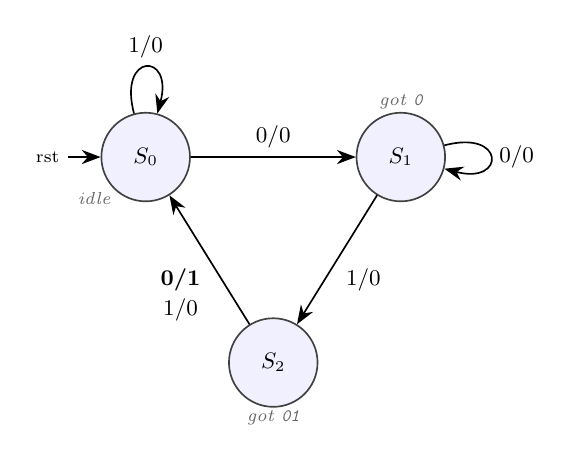
\begin{tikzpicture}[fsm,scale=0.90,transform shape]
\node[state,initial,label={[meaning]below left:{\textit{idle}}}] (S0) at (0.00,0.00) {$S_{0}$};
\node[state,label={[meaning]above:{got \texttt{0}}}] (S1) at (3.60,0.00) {$S_{1}$};
\node[state,label={[meaning]below:{got \texttt{01}}}] (S2) at (1.80,-2.90) {$S_{2}$};
\path (S0) edge[loop above] node[elab] {1/0} (S0);
\path (S0) edge[] node[elab] {0/0} (S1);
\path (S1) edge[loop right] node[elab] {0/0} (S1);
\path (S1) edge[] node[elab] {1/0} (S2);
\path (S2) edge[] node[elab] {\shortstack{\textbf{0/1}\\1/0}} (S0);
\end{tikzpicture}
\end{center}
\begin{codeslice}{Mealy version -- 3 states, output on the transition}{seq010\_mealy.v}
\slicenote{Same detector with one state fewer; \texttt{det\_out} rises in the same clock as the final 0.}
\begin{lstlisting}
`timescale 1ns/1ps
// Non-overlapping "010" sequence detector -- Mealy FSM
module seq010_mealy (
    input  wire clk,
    input  wire rst,
    input  wire serin,
    output reg  det_out
);
    localparam [1:0] S0 = 2'd0,    // idle
                     S1 = 2'd1,    // got "0"
                     S2 = 2'd2;    // got "01"
    reg [1:0] state, next_state;

    always @(posedge clk or posedge rst)
        if (rst) state <= S0;
        else     state <= next_state;

    // next state AND output in one combinational block
    always @(*) begin
        next_state = S0;
        det_out    = 1'b0;
        case (state)
            S0: next_state = serin ? S0 : S1;
            S1: next_state = serin ? S2 : S1;
            S2: begin
                    next_state = S0;        // 011 -> idle, 010 -> idle (non-overlap)
                    det_out    = ~serin;    // "01" followed by 0: detected NOW
                end
            default: next_state = S0;
        endcase
    end
endmodule
\end{lstlisting}
\end{codeslice}

\subsection{Testbench -- 100 random clocks, slice by slice}
\begin{codeslice}{TB slice 1 -- signals, DUT and clock}{tb\_seq010.v}
\slicenote{The testbench has no ports. Inputs are \texttt{reg}, outputs are \texttt{wire}.}
\begin{lstlisting}
`timescale 1ns/1ps
module tb_seq010;
    reg  clk = 1'b0, rst = 1'b1, serin = 1'b0;
    wire det_out;
    integer i, hits = 0, errors = 0;
    reg [1:0] hist;  integer n;  reg exp;     // golden model (slice 4)

    seq010_moore dut (.clk(clk), .rst(rst), .serin(serin), .det_out(det_out));

    always #5 clk = ~clk;                     // 10 ns clock period
\end{lstlisting}
\end{codeslice}
\begin{codeslice}{TB slice 2 -- reset, then 100 clocks of random input}{tb\_seq010.v}
\slicenote{Change the input 1\,ns after the rising edge so it never races the clock.}
\begin{lstlisting}
    initial begin
        $dumpfile("tb_seq010.vcd");           // open in GTKWave
        $dumpvars(0, tb_seq010);
        repeat (2) @(posedge clk);            // hold reset for 2 clocks
        #1 rst = 1'b0;
        for (i = 0; i < 100; i = i + 1) begin
            serin = $random;                  // LSB of a random number: 0/1
            @(posedge clk); #1;               // held for exactly one clock
        end
        $display("DONE: %0d detections, %0d errors", hits, errors);
        $finish;
    end
\end{lstlisting}
\end{codeslice}
\begin{codeslice}{TB slice 3 -- print what happens on every clock}{tb\_seq010.v}
\slicenote{\texttt{\$strobe} prints at the end of the time step, so it shows the new state.}
\begin{lstlisting}
    always @(posedge clk)
        if (!rst)
            $strobe("%6t  serin=%b  ->  state=S%0d  det_out=%b",
                    $time, serin, dut.state, det_out);
\end{lstlisting}
\end{codeslice}
\begin{codeslice}{TB slice 4 -- self-check against a golden model (bonus marks)}{tb\_seq010.v}
\slicenote{Keep the last 2 bits and count fresh bits since the last hit. The non-overlap rule is that a hit needs 3 fresh bits.}
\begin{lstlisting}
    always @(posedge clk or posedge rst)
        if (rst) begin
            hist <= 2'b00;  n <= 0;  exp <= 1'b0;
        end else begin
            hist <= {hist[0], serin};
            if (n >= 2 && {hist, serin} == 3'b010) begin
                exp <= 1'b1;  n <= 0;                 // hit: restart counting
            end else begin
                exp <= 1'b0;  n <= (n < 2) ? n + 1 : n;
            end
        end

    always @(negedge clk)                     // compare mid-cycle
        if (!rst) begin
            if (det_out) hits = hits + 1;
            if (det_out !== exp) begin
                errors = errors + 1;
                $display("MISMATCH at %0t: det_out=%b expected=%b",
                         $time, det_out, exp);
            end
        end
endmodule
\end{lstlisting}
\end{codeslice}


\newpage
\section{Q1 (given) -- ``01'' on a 2-bit \texttt{serin} for 3 consecutive clocks, overlap allowed}
\begin{qbox}{Question}
Write a synthesizable behavioral model of an FSM that asserts an output \texttt{det\_out} if the value ``01''
is received in a 2-bit input \texttt{serin} for three consecutive clocks with overlaps allowed. Write a test
bench for verifying the FSM with random inputs applied for 100 clocks.
\end{qbox}

\subsection{Key idea: this is a counter, not a bit pattern}
Here \texttt{serin} is a 2-bit \emph{bus}, and ``01'' is one value of it (\texttt{2'b01}). The FSM only has to
count how many clocks \emph{in a row} it has seen \texttt{01}. Any other value (00, 10, 11) breaks the run.
\emph{Overlap allowed} means a 4th consecutive 01 is a new run of three (clocks 2--4), so \texttt{det\_out}
stays high, which is the self-loop on $S_3$.

\begin{center}\small
\begin{tabular}{c l c c}
\toprule
State & Meaning & \texttt{serin}=01 & \texttt{serin}$\neq$01 \\ \midrule
$S_0$ & 0 in a row & $S_1$ & $S_0$ \\
$S_1$ & 1 in a row & $S_2$ & $S_0$ \\
$S_2$ & 2 in a row & $S_3$ & $S_0$ \\
\rowcolor{orange!15} $S_3$ & $\geq$3 in a row, \textbf{det\_out=1} & $S_3$ (overlap) & $S_0$ \\
\bottomrule
\end{tabular}
\end{center}
{\small Non-overlapping variant: $S_3 \xrightarrow{01} S_1$ (the run restarts at 1).}

\subsection{State diagram (Moore)}
\begin{center}
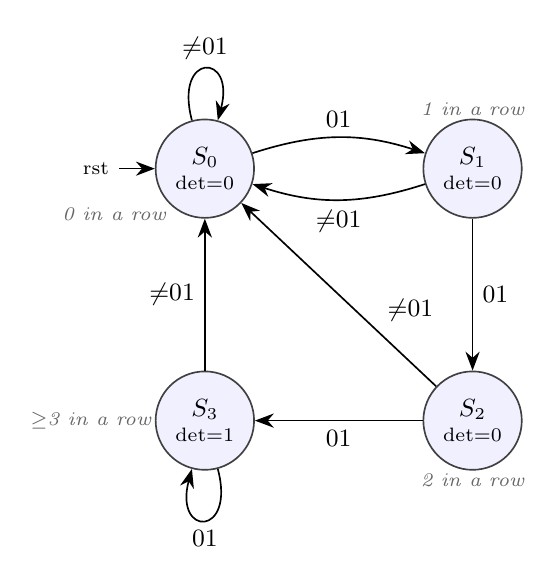
\begin{tikzpicture}[fsm,scale=1.00,transform shape]
\node[state,initial,label={[meaning]below left:{\textit{0 in a row}}}] (S0) at (0.00,0.00) {$S_{0}$\\[-2pt]{\scriptsize det=0}};
\node[state,label={[meaning]above:{\textit{1 in a row}}}] (S1) at (3.40,0.00) {$S_{1}$\\[-2pt]{\scriptsize det=0}};
\node[state,label={[meaning]below:{\textit{2 in a row}}}] (S2) at (3.40,-3.20) {$S_{2}$\\[-2pt]{\scriptsize det=0}};
\node[state,label={[meaning]left:{\textit{$\geq$3 in a row}}}] (S3) at (0.00,-3.20) {$S_{3}$\\[-2pt]{\scriptsize det=1}};
\path (S0) edge[loop above] node[elab] {$\neq$01} (S0);
\path (S0) edge[bend left=18] node[elab] {01} (S1);
\path (S1) edge[bend left=18] node[elab] {$\neq$01} (S0);
\path (S1) edge[] node[elab] {01} (S2);
\path (S2) edge[] node[elab] {01} (S3);
\path (S2) edge[] node[elab,pos=0.3,swap] {$\neq$01} (S0);
\path (S3) edge[loop below] node[elab] {01} (S3);
\path (S3) edge[] node[elab] {$\neq$01} (S0);
\end{tikzpicture}
\end{center}

\subsection{Step-by-step}
{\small Legend for the step-by-step pictures: \tikz\node[draw=black!75,fill=yellow!75,circle,minimum size=3mm,inner sep=0]{};~present state \quad \tikz\node[draw=red!80!black,line width=1.6pt,fill=blue!6,circle,minimum size=3mm,inner sep=0]{};~next state \quad \tikz\draw[->,>=Stealth,red!80!black,line width=1.6pt](0,0)--(0.6,0);~transition taken on this clock edge}\par\smallskip\noindent
\begin{minipage}[t]{0.327\textwidth}\centering
\fcolorbox{black!15}{white}{\begin{minipage}{0.94\linewidth}\centering
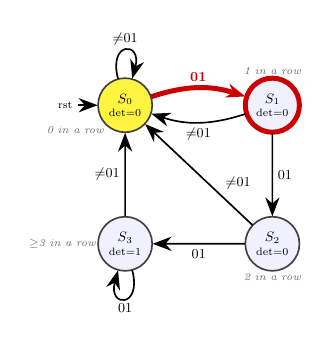
\begin{tikzpicture}[fsm,scale=0.55,transform shape]
\node[state,initial,cur,label={[meaning]below left:{\textit{0 in a row}}}] (S0) at (0.00,0.00) {$S_{0}$\\[-2pt]{\scriptsize det=0}};
\node[state,nxt,label={[meaning]above:{\textit{1 in a row}}}] (S1) at (3.40,0.00) {$S_{1}$\\[-2pt]{\scriptsize det=0}};
\node[state,label={[meaning]below:{\textit{2 in a row}}}] (S2) at (3.40,-3.20) {$S_{2}$\\[-2pt]{\scriptsize det=0}};
\node[state,label={[meaning]left:{\textit{$\geq$3 in a row}}}] (S3) at (0.00,-3.20) {$S_{3}$\\[-2pt]{\scriptsize det=1}};
\path (S0) edge[loop above] node[elab] {$\neq$01} (S0);
\path (S0) edge[bend left=18,hl] node[elab,hlnode] {01} (S1);
\path (S1) edge[bend left=18] node[elab] {$\neq$01} (S0);
\path (S1) edge[] node[elab] {01} (S2);
\path (S2) edge[] node[elab] {01} (S3);
\path (S2) edge[] node[elab,pos=0.3,swap] {$\neq$01} (S0);
\path (S3) edge[loop below] node[elab] {01} (S3);
\path (S3) edge[] node[elab] {$\neq$01} (S0);
\end{tikzpicture}
\\[2pt]{\small\textbf{Clock 1}: \texttt{serin=01}}\\[1pt]{\scriptsize $S_{0}$ $\rightarrow$ $S_{1}$ \;|\; det\_out=0 {\tiny(after edge)}}\end{minipage}}\end{minipage}
\hfill
\begin{minipage}[t]{0.327\textwidth}\centering
\fcolorbox{black!15}{white}{\begin{minipage}{0.94\linewidth}\centering
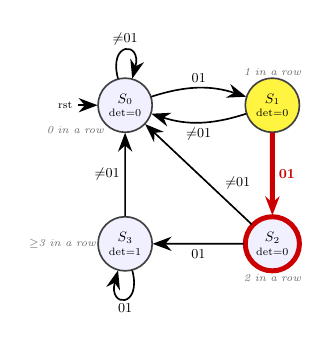
\begin{tikzpicture}[fsm,scale=0.55,transform shape]
\node[state,initial,label={[meaning]below left:{\textit{0 in a row}}}] (S0) at (0.00,0.00) {$S_{0}$\\[-2pt]{\scriptsize det=0}};
\node[state,cur,label={[meaning]above:{\textit{1 in a row}}}] (S1) at (3.40,0.00) {$S_{1}$\\[-2pt]{\scriptsize det=0}};
\node[state,nxt,label={[meaning]below:{\textit{2 in a row}}}] (S2) at (3.40,-3.20) {$S_{2}$\\[-2pt]{\scriptsize det=0}};
\node[state,label={[meaning]left:{\textit{$\geq$3 in a row}}}] (S3) at (0.00,-3.20) {$S_{3}$\\[-2pt]{\scriptsize det=1}};
\path (S0) edge[loop above] node[elab] {$\neq$01} (S0);
\path (S0) edge[bend left=18] node[elab] {01} (S1);
\path (S1) edge[bend left=18] node[elab] {$\neq$01} (S0);
\path (S1) edge[hl] node[elab,hlnode] {01} (S2);
\path (S2) edge[] node[elab] {01} (S3);
\path (S2) edge[] node[elab,pos=0.3,swap] {$\neq$01} (S0);
\path (S3) edge[loop below] node[elab] {01} (S3);
\path (S3) edge[] node[elab] {$\neq$01} (S0);
\end{tikzpicture}
\\[2pt]{\small\textbf{Clock 2}: \texttt{serin=01}}\\[1pt]{\scriptsize $S_{1}$ $\rightarrow$ $S_{2}$ \;|\; det\_out=0 {\tiny(after edge)}}\end{minipage}}\end{minipage}
\hfill
\begin{minipage}[t]{0.327\textwidth}\centering
\fcolorbox{black!15}{white}{\begin{minipage}{0.94\linewidth}\centering
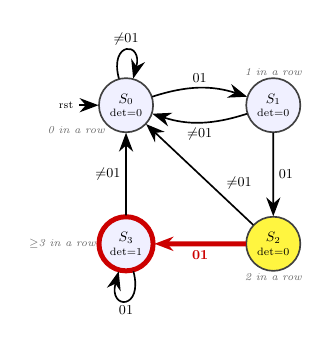
\begin{tikzpicture}[fsm,scale=0.55,transform shape]
\node[state,initial,label={[meaning]below left:{\textit{0 in a row}}}] (S0) at (0.00,0.00) {$S_{0}$\\[-2pt]{\scriptsize det=0}};
\node[state,label={[meaning]above:{\textit{1 in a row}}}] (S1) at (3.40,0.00) {$S_{1}$\\[-2pt]{\scriptsize det=0}};
\node[state,cur,label={[meaning]below:{\textit{2 in a row}}}] (S2) at (3.40,-3.20) {$S_{2}$\\[-2pt]{\scriptsize det=0}};
\node[state,nxt,label={[meaning]left:{\textit{$\geq$3 in a row}}}] (S3) at (0.00,-3.20) {$S_{3}$\\[-2pt]{\scriptsize det=1}};
\path (S0) edge[loop above] node[elab] {$\neq$01} (S0);
\path (S0) edge[bend left=18] node[elab] {01} (S1);
\path (S1) edge[bend left=18] node[elab] {$\neq$01} (S0);
\path (S1) edge[] node[elab] {01} (S2);
\path (S2) edge[hl] node[elab,hlnode] {01} (S3);
\path (S2) edge[] node[elab,pos=0.3,swap] {$\neq$01} (S0);
\path (S3) edge[loop below] node[elab] {01} (S3);
\path (S3) edge[] node[elab] {$\neq$01} (S0);
\end{tikzpicture}
\\[2pt]{\small\textbf{Clock 3}: \texttt{serin=01}}\\[1pt]{\scriptsize $S_{2}$ $\rightarrow$ $S_{3}$ \;|\; \textcolor{red!80!black}{\textbf{det\_out=1}} {\tiny(after edge)}}\end{minipage}}\end{minipage}
\par\medskip\noindent
\begin{minipage}[t]{0.327\textwidth}\centering
\fcolorbox{black!15}{white}{\begin{minipage}{0.94\linewidth}\centering
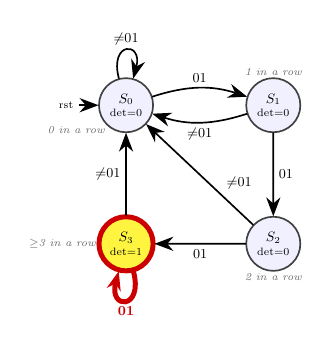
\begin{tikzpicture}[fsm,scale=0.55,transform shape]
\node[state,initial,label={[meaning]below left:{\textit{0 in a row}}}] (S0) at (0.00,0.00) {$S_{0}$\\[-2pt]{\scriptsize det=0}};
\node[state,label={[meaning]above:{\textit{1 in a row}}}] (S1) at (3.40,0.00) {$S_{1}$\\[-2pt]{\scriptsize det=0}};
\node[state,label={[meaning]below:{\textit{2 in a row}}}] (S2) at (3.40,-3.20) {$S_{2}$\\[-2pt]{\scriptsize det=0}};
\node[state,cur,nxt,label={[meaning]left:{\textit{$\geq$3 in a row}}}] (S3) at (0.00,-3.20) {$S_{3}$\\[-2pt]{\scriptsize det=1}};
\path (S0) edge[loop above] node[elab] {$\neq$01} (S0);
\path (S0) edge[bend left=18] node[elab] {01} (S1);
\path (S1) edge[bend left=18] node[elab] {$\neq$01} (S0);
\path (S1) edge[] node[elab] {01} (S2);
\path (S2) edge[] node[elab] {01} (S3);
\path (S2) edge[] node[elab,pos=0.3,swap] {$\neq$01} (S0);
\path (S3) edge[loop below,hl] node[elab,hlnode] {01} (S3);
\path (S3) edge[] node[elab] {$\neq$01} (S0);
\end{tikzpicture}
\\[2pt]{\small\textbf{Clock 4}: \texttt{serin=01}}\\[1pt]{\scriptsize $S_{3}$ $\rightarrow$ $S_{3}$ \;|\; \textcolor{red!80!black}{\textbf{det\_out=1}} {\tiny(after edge)}}\end{minipage}}\end{minipage}
\hfill
\begin{minipage}[t]{0.327\textwidth}\centering
\fcolorbox{black!15}{white}{\begin{minipage}{0.94\linewidth}\centering
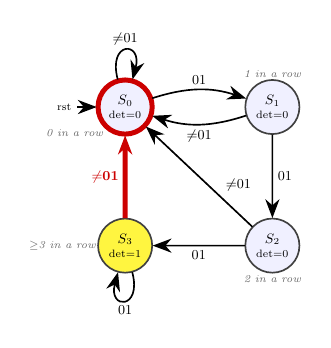
\begin{tikzpicture}[fsm,scale=0.55,transform shape]
\node[state,initial,nxt,label={[meaning]below left:{\textit{0 in a row}}}] (S0) at (0.00,0.00) {$S_{0}$\\[-2pt]{\scriptsize det=0}};
\node[state,label={[meaning]above:{\textit{1 in a row}}}] (S1) at (3.40,0.00) {$S_{1}$\\[-2pt]{\scriptsize det=0}};
\node[state,label={[meaning]below:{\textit{2 in a row}}}] (S2) at (3.40,-3.20) {$S_{2}$\\[-2pt]{\scriptsize det=0}};
\node[state,cur,label={[meaning]left:{\textit{$\geq$3 in a row}}}] (S3) at (0.00,-3.20) {$S_{3}$\\[-2pt]{\scriptsize det=1}};
\path (S0) edge[loop above] node[elab] {$\neq$01} (S0);
\path (S0) edge[bend left=18] node[elab] {01} (S1);
\path (S1) edge[bend left=18] node[elab] {$\neq$01} (S0);
\path (S1) edge[] node[elab] {01} (S2);
\path (S2) edge[] node[elab] {01} (S3);
\path (S2) edge[] node[elab,pos=0.3,swap] {$\neq$01} (S0);
\path (S3) edge[loop below] node[elab] {01} (S3);
\path (S3) edge[hl] node[elab,hlnode] {$\neq$01} (S0);
\end{tikzpicture}
\\[2pt]{\small\textbf{Clock 5}: \texttt{serin=10}}\\[1pt]{\scriptsize $S_{3}$ $\rightarrow$ $S_{0}$ \;|\; det\_out=0 {\tiny(after edge)}}\end{minipage}}\end{minipage}
\hfill
\begin{minipage}[t]{0.327\textwidth}\centering
\fcolorbox{black!15}{white}{\begin{minipage}{0.94\linewidth}\centering
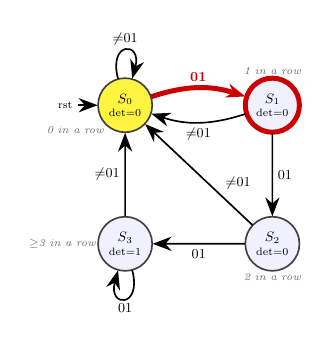
\begin{tikzpicture}[fsm,scale=0.55,transform shape]
\node[state,initial,cur,label={[meaning]below left:{\textit{0 in a row}}}] (S0) at (0.00,0.00) {$S_{0}$\\[-2pt]{\scriptsize det=0}};
\node[state,nxt,label={[meaning]above:{\textit{1 in a row}}}] (S1) at (3.40,0.00) {$S_{1}$\\[-2pt]{\scriptsize det=0}};
\node[state,label={[meaning]below:{\textit{2 in a row}}}] (S2) at (3.40,-3.20) {$S_{2}$\\[-2pt]{\scriptsize det=0}};
\node[state,label={[meaning]left:{\textit{$\geq$3 in a row}}}] (S3) at (0.00,-3.20) {$S_{3}$\\[-2pt]{\scriptsize det=1}};
\path (S0) edge[loop above] node[elab] {$\neq$01} (S0);
\path (S0) edge[bend left=18,hl] node[elab,hlnode] {01} (S1);
\path (S1) edge[bend left=18] node[elab] {$\neq$01} (S0);
\path (S1) edge[] node[elab] {01} (S2);
\path (S2) edge[] node[elab] {01} (S3);
\path (S2) edge[] node[elab,pos=0.3,swap] {$\neq$01} (S0);
\path (S3) edge[loop below] node[elab] {01} (S3);
\path (S3) edge[] node[elab] {$\neq$01} (S0);
\end{tikzpicture}
\\[2pt]{\small\textbf{Clock 6}: \texttt{serin=01}}\\[1pt]{\scriptsize $S_{0}$ $\rightarrow$ $S_{1}$ \;|\; det\_out=0 {\tiny(after edge)}}\end{minipage}}\end{minipage}
\par\medskip\noindent
\begin{minipage}[t]{0.327\textwidth}\centering
\fcolorbox{black!15}{white}{\begin{minipage}{0.94\linewidth}\centering
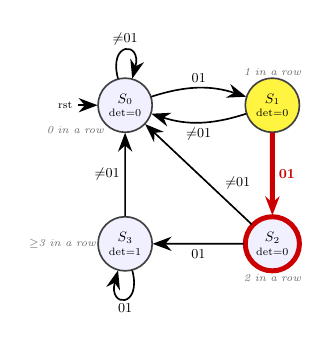
\begin{tikzpicture}[fsm,scale=0.55,transform shape]
\node[state,initial,label={[meaning]below left:{\textit{0 in a row}}}] (S0) at (0.00,0.00) {$S_{0}$\\[-2pt]{\scriptsize det=0}};
\node[state,cur,label={[meaning]above:{\textit{1 in a row}}}] (S1) at (3.40,0.00) {$S_{1}$\\[-2pt]{\scriptsize det=0}};
\node[state,nxt,label={[meaning]below:{\textit{2 in a row}}}] (S2) at (3.40,-3.20) {$S_{2}$\\[-2pt]{\scriptsize det=0}};
\node[state,label={[meaning]left:{\textit{$\geq$3 in a row}}}] (S3) at (0.00,-3.20) {$S_{3}$\\[-2pt]{\scriptsize det=1}};
\path (S0) edge[loop above] node[elab] {$\neq$01} (S0);
\path (S0) edge[bend left=18] node[elab] {01} (S1);
\path (S1) edge[bend left=18] node[elab] {$\neq$01} (S0);
\path (S1) edge[hl] node[elab,hlnode] {01} (S2);
\path (S2) edge[] node[elab] {01} (S3);
\path (S2) edge[] node[elab,pos=0.3,swap] {$\neq$01} (S0);
\path (S3) edge[loop below] node[elab] {01} (S3);
\path (S3) edge[] node[elab] {$\neq$01} (S0);
\end{tikzpicture}
\\[2pt]{\small\textbf{Clock 7}: \texttt{serin=01}}\\[1pt]{\scriptsize $S_{1}$ $\rightarrow$ $S_{2}$ \;|\; det\_out=0 {\tiny(after edge)}}\end{minipage}}\end{minipage}
\hfill
\begin{minipage}[t]{0.327\textwidth}\centering
\fcolorbox{black!15}{white}{\begin{minipage}{0.94\linewidth}\centering
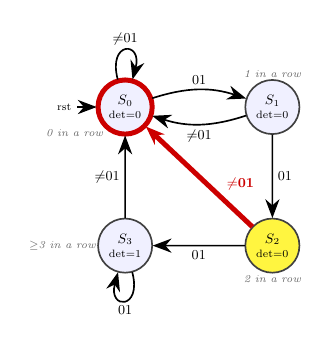
\begin{tikzpicture}[fsm,scale=0.55,transform shape]
\node[state,initial,nxt,label={[meaning]below left:{\textit{0 in a row}}}] (S0) at (0.00,0.00) {$S_{0}$\\[-2pt]{\scriptsize det=0}};
\node[state,label={[meaning]above:{\textit{1 in a row}}}] (S1) at (3.40,0.00) {$S_{1}$\\[-2pt]{\scriptsize det=0}};
\node[state,cur,label={[meaning]below:{\textit{2 in a row}}}] (S2) at (3.40,-3.20) {$S_{2}$\\[-2pt]{\scriptsize det=0}};
\node[state,label={[meaning]left:{\textit{$\geq$3 in a row}}}] (S3) at (0.00,-3.20) {$S_{3}$\\[-2pt]{\scriptsize det=1}};
\path (S0) edge[loop above] node[elab] {$\neq$01} (S0);
\path (S0) edge[bend left=18] node[elab] {01} (S1);
\path (S1) edge[bend left=18] node[elab] {$\neq$01} (S0);
\path (S1) edge[] node[elab] {01} (S2);
\path (S2) edge[] node[elab] {01} (S3);
\path (S2) edge[hl] node[elab,pos=0.3,swap,hlnode] {$\neq$01} (S0);
\path (S3) edge[loop below] node[elab] {01} (S3);
\path (S3) edge[] node[elab] {$\neq$01} (S0);
\end{tikzpicture}
\\[2pt]{\small\textbf{Clock 8}: \texttt{serin=00}}\\[1pt]{\scriptsize $S_{2}$ $\rightarrow$ $S_{0}$ \;|\; det\_out=0 {\tiny(after edge)}}\end{minipage}}\end{minipage}
\hfill
\begin{minipage}[t]{0.327\textwidth}\centering
\fcolorbox{black!15}{white}{\begin{minipage}{0.94\linewidth}\centering
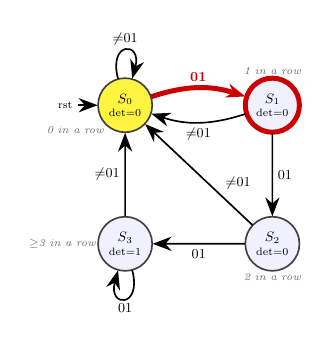
\begin{tikzpicture}[fsm,scale=0.55,transform shape]
\node[state,initial,cur,label={[meaning]below left:{\textit{0 in a row}}}] (S0) at (0.00,0.00) {$S_{0}$\\[-2pt]{\scriptsize det=0}};
\node[state,nxt,label={[meaning]above:{\textit{1 in a row}}}] (S1) at (3.40,0.00) {$S_{1}$\\[-2pt]{\scriptsize det=0}};
\node[state,label={[meaning]below:{\textit{2 in a row}}}] (S2) at (3.40,-3.20) {$S_{2}$\\[-2pt]{\scriptsize det=0}};
\node[state,label={[meaning]left:{\textit{$\geq$3 in a row}}}] (S3) at (0.00,-3.20) {$S_{3}$\\[-2pt]{\scriptsize det=1}};
\path (S0) edge[loop above] node[elab] {$\neq$01} (S0);
\path (S0) edge[bend left=18,hl] node[elab,hlnode] {01} (S1);
\path (S1) edge[bend left=18] node[elab] {$\neq$01} (S0);
\path (S1) edge[] node[elab] {01} (S2);
\path (S2) edge[] node[elab] {01} (S3);
\path (S2) edge[] node[elab,pos=0.3,swap] {$\neq$01} (S0);
\path (S3) edge[loop below] node[elab] {01} (S3);
\path (S3) edge[] node[elab] {$\neq$01} (S0);
\end{tikzpicture}
\\[2pt]{\small\textbf{Clock 9}: \texttt{serin=01}}\\[1pt]{\scriptsize $S_{0}$ $\rightarrow$ $S_{1}$ \;|\; det\_out=0 {\tiny(after edge)}}\end{minipage}}\end{minipage}
\par\medskip\noindent

\subsection{Trace table}
\begin{center}\small
\begin{tabular}{c c c c c}
\toprule
Clock edge & \texttt{serin} sampled & Present state & Next state & \texttt{det\_out} {\scriptsize after edge (Moore)}\\
\midrule
1 & \texttt{01} & $S_{0}$ & $S_{1}$ & 0\\
2 & \texttt{01} & $S_{1}$ & $S_{2}$ & 0\\
\rowcolor{red!12}3 & \texttt{01} & $S_{2}$ & $S_{3}$ & \textbf{1}\\
\rowcolor{red!12}4 & \texttt{01} & $S_{3}$ & $S_{3}$ & \textbf{1}\\
5 & \texttt{10} & $S_{3}$ & $S_{0}$ & 0\\
6 & \texttt{01} & $S_{0}$ & $S_{1}$ & 0\\
7 & \texttt{01} & $S_{1}$ & $S_{2}$ & 0\\
8 & \texttt{00} & $S_{2}$ & $S_{0}$ & 0\\
9 & \texttt{01} & $S_{0}$ & $S_{1}$ & 0\\
10 & \texttt{01} & $S_{1}$ & $S_{2}$ & 0\\
\rowcolor{red!12}11 & \texttt{01} & $S_{2}$ & $S_{3}$ & \textbf{1}\\
12 & \texttt{11} & $S_{3}$ & $S_{0}$ & 0\\
13 & \texttt{01} & $S_{0}$ & $S_{1}$ & 0\\
14 & \texttt{01} & $S_{1}$ & $S_{2}$ & 0\\
\rowcolor{red!12}15 & \texttt{01} & $S_{2}$ & $S_{3}$ & \textbf{1}\\
\rowcolor{red!12}16 & \texttt{01} & $S_{3}$ & $S_{3}$ & \textbf{1}\\
\rowcolor{red!12}17 & \texttt{01} & $S_{3}$ & $S_{3}$ & \textbf{1}\\
18 & \texttt{10} & $S_{3}$ & $S_{0}$ & 0\\
19 & \texttt{00} & $S_{0}$ & $S_{0}$ & 0\\
20 & \texttt{01} & $S_{0}$ & $S_{1}$ & 0\\
\bottomrule
\end{tabular}\end{center}

\subsection{Waveform}
\begin{center}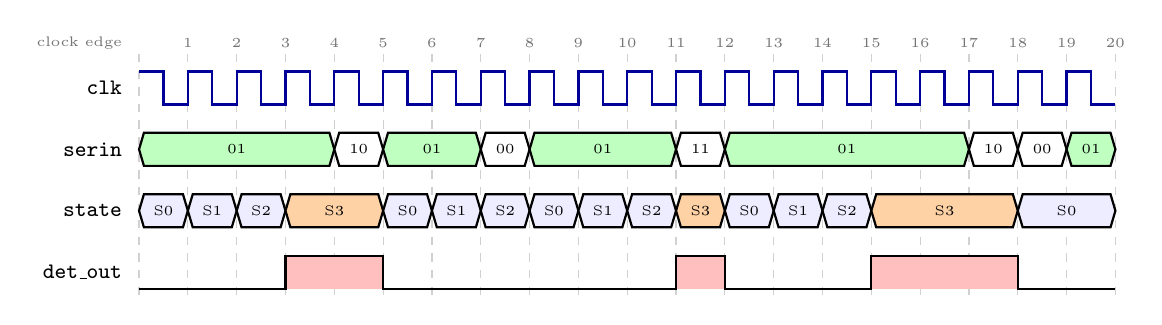
\begin{tikzpicture}[x=0.62cm,y=1cm,font=\scriptsize]
\draw[black!18,dashed] (0,0.64)--(0,-2.44);
\draw[black!18,dashed] (1,0.64)--(1,-2.44);
\node[black!55,font=\tiny] at (1,0.78) {1};
\draw[black!18,dashed] (2,0.64)--(2,-2.44);
\node[black!55,font=\tiny] at (2,0.78) {2};
\draw[black!18,dashed] (3,0.64)--(3,-2.44);
\node[black!55,font=\tiny] at (3,0.78) {3};
\draw[black!18,dashed] (4,0.64)--(4,-2.44);
\node[black!55,font=\tiny] at (4,0.78) {4};
\draw[black!18,dashed] (5,0.64)--(5,-2.44);
\node[black!55,font=\tiny] at (5,0.78) {5};
\draw[black!18,dashed] (6,0.64)--(6,-2.44);
\node[black!55,font=\tiny] at (6,0.78) {6};
\draw[black!18,dashed] (7,0.64)--(7,-2.44);
\node[black!55,font=\tiny] at (7,0.78) {7};
\draw[black!18,dashed] (8,0.64)--(8,-2.44);
\node[black!55,font=\tiny] at (8,0.78) {8};
\draw[black!18,dashed] (9,0.64)--(9,-2.44);
\node[black!55,font=\tiny] at (9,0.78) {9};
\draw[black!18,dashed] (10,0.64)--(10,-2.44);
\node[black!55,font=\tiny] at (10,0.78) {10};
\draw[black!18,dashed] (11,0.64)--(11,-2.44);
\node[black!55,font=\tiny] at (11,0.78) {11};
\draw[black!18,dashed] (12,0.64)--(12,-2.44);
\node[black!55,font=\tiny] at (12,0.78) {12};
\draw[black!18,dashed] (13,0.64)--(13,-2.44);
\node[black!55,font=\tiny] at (13,0.78) {13};
\draw[black!18,dashed] (14,0.64)--(14,-2.44);
\node[black!55,font=\tiny] at (14,0.78) {14};
\draw[black!18,dashed] (15,0.64)--(15,-2.44);
\node[black!55,font=\tiny] at (15,0.78) {15};
\draw[black!18,dashed] (16,0.64)--(16,-2.44);
\node[black!55,font=\tiny] at (16,0.78) {16};
\draw[black!18,dashed] (17,0.64)--(17,-2.44);
\node[black!55,font=\tiny] at (17,0.78) {17};
\draw[black!18,dashed] (18,0.64)--(18,-2.44);
\node[black!55,font=\tiny] at (18,0.78) {18};
\draw[black!18,dashed] (19,0.64)--(19,-2.44);
\node[black!55,font=\tiny] at (19,0.78) {19};
\draw[black!18,dashed] (20,0.64)--(20,-2.44);
\node[black!55,font=\tiny] at (20,0.78) {20};
\node[anchor=east,black!55,font=\tiny] at (-0.15,0.78) {clock edge};
\node[anchor=east,font=\footnotesize\ttfamily] at (-0.15,0.21) {clk};
\draw[thick,blue!60!black] (0.000,0.420) -- (0.500,0.420) -- (0.500,0.000) -- (1.000,0.000) -- (1.000,0.420) -- (1.500,0.420) -- (1.500,0.000) -- (2.000,0.000) -- (2.000,0.420) -- (2.500,0.420) -- (2.500,0.000) -- (3.000,0.000) -- (3.000,0.420) -- (3.500,0.420) -- (3.500,0.000) -- (4.000,0.000) -- (4.000,0.420) -- (4.500,0.420) -- (4.500,0.000) -- (5.000,0.000) -- (5.000,0.420) -- (5.500,0.420) -- (5.500,0.000) -- (6.000,0.000) -- (6.000,0.420) -- (6.500,0.420) -- (6.500,0.000) -- (7.000,0.000) -- (7.000,0.420) -- (7.500,0.420) -- (7.500,0.000) -- (8.000,0.000) -- (8.000,0.420) -- (8.500,0.420) -- (8.500,0.000) -- (9.000,0.000) -- (9.000,0.420) -- (9.500,0.420) -- (9.500,0.000) -- (10.000,0.000) -- (10.000,0.420) -- (10.500,0.420) -- (10.500,0.000) -- (11.000,0.000) -- (11.000,0.420) -- (11.500,0.420) -- (11.500,0.000) -- (12.000,0.000) -- (12.000,0.420) -- (12.500,0.420) -- (12.500,0.000) -- (13.000,0.000) -- (13.000,0.420) -- (13.500,0.420) -- (13.500,0.000) -- (14.000,0.000) -- (14.000,0.420) -- (14.500,0.420) -- (14.500,0.000) -- (15.000,0.000) -- (15.000,0.420) -- (15.500,0.420) -- (15.500,0.000) -- (16.000,0.000) -- (16.000,0.420) -- (16.500,0.420) -- (16.500,0.000) -- (17.000,0.000) -- (17.000,0.420) -- (17.500,0.420) -- (17.500,0.000) -- (18.000,0.000) -- (18.000,0.420) -- (18.500,0.420) -- (18.500,0.000) -- (19.000,0.000) -- (19.000,0.420) -- (19.500,0.420) -- (19.500,0.000) -- (20.000,0.000);
\node[anchor=east,font=\footnotesize\ttfamily] at (-0.15,-0.57) {serin};
\draw[thick,fill=green!25] (0.000,-0.570)--(0.100,-0.360)--(3.900,-0.360)--(4.000,-0.570)--(3.900,-0.780)--(0.100,-0.780)--cycle;
\node[font=\tiny] at (2.000,-0.570) {01};
\draw[thick,fill=white] (4.000,-0.570)--(4.100,-0.360)--(4.900,-0.360)--(5.000,-0.570)--(4.900,-0.780)--(4.100,-0.780)--cycle;
\node[font=\tiny] at (4.500,-0.570) {10};
\draw[thick,fill=green!25] (5.000,-0.570)--(5.100,-0.360)--(6.900,-0.360)--(7.000,-0.570)--(6.900,-0.780)--(5.100,-0.780)--cycle;
\node[font=\tiny] at (6.000,-0.570) {01};
\draw[thick,fill=white] (7.000,-0.570)--(7.100,-0.360)--(7.900,-0.360)--(8.000,-0.570)--(7.900,-0.780)--(7.100,-0.780)--cycle;
\node[font=\tiny] at (7.500,-0.570) {00};
\draw[thick,fill=green!25] (8.000,-0.570)--(8.100,-0.360)--(10.900,-0.360)--(11.000,-0.570)--(10.900,-0.780)--(8.100,-0.780)--cycle;
\node[font=\tiny] at (9.500,-0.570) {01};
\draw[thick,fill=white] (11.000,-0.570)--(11.100,-0.360)--(11.900,-0.360)--(12.000,-0.570)--(11.900,-0.780)--(11.100,-0.780)--cycle;
\node[font=\tiny] at (11.500,-0.570) {11};
\draw[thick,fill=green!25] (12.000,-0.570)--(12.100,-0.360)--(16.900,-0.360)--(17.000,-0.570)--(16.900,-0.780)--(12.100,-0.780)--cycle;
\node[font=\tiny] at (14.500,-0.570) {01};
\draw[thick,fill=white] (17.000,-0.570)--(17.100,-0.360)--(17.900,-0.360)--(18.000,-0.570)--(17.900,-0.780)--(17.100,-0.780)--cycle;
\node[font=\tiny] at (17.500,-0.570) {10};
\draw[thick,fill=white] (18.000,-0.570)--(18.100,-0.360)--(18.900,-0.360)--(19.000,-0.570)--(18.900,-0.780)--(18.100,-0.780)--cycle;
\node[font=\tiny] at (18.500,-0.570) {00};
\draw[thick,fill=green!25] (19.000,-0.570)--(19.100,-0.360)--(19.900,-0.360)--(20.000,-0.570)--(19.900,-0.780)--(19.100,-0.780)--cycle;
\node[font=\tiny] at (19.500,-0.570) {01};
\node[anchor=east,font=\footnotesize\ttfamily] at (-0.15,-1.35) {state};
\draw[thick,fill=blue!7] (0.000,-1.350)--(0.100,-1.140)--(0.900,-1.140)--(1.000,-1.350)--(0.900,-1.560)--(0.100,-1.560)--cycle;
\node[font=\tiny] at (0.500,-1.350) {S0};
\draw[thick,fill=blue!7] (1.000,-1.350)--(1.100,-1.140)--(1.900,-1.140)--(2.000,-1.350)--(1.900,-1.560)--(1.100,-1.560)--cycle;
\node[font=\tiny] at (1.500,-1.350) {S1};
\draw[thick,fill=blue!7] (2.000,-1.350)--(2.100,-1.140)--(2.900,-1.140)--(3.000,-1.350)--(2.900,-1.560)--(2.100,-1.560)--cycle;
\node[font=\tiny] at (2.500,-1.350) {S2};
\draw[thick,fill=orange!35] (3.000,-1.350)--(3.100,-1.140)--(4.900,-1.140)--(5.000,-1.350)--(4.900,-1.560)--(3.100,-1.560)--cycle;
\node[font=\tiny] at (4.000,-1.350) {S3};
\draw[thick,fill=blue!7] (5.000,-1.350)--(5.100,-1.140)--(5.900,-1.140)--(6.000,-1.350)--(5.900,-1.560)--(5.100,-1.560)--cycle;
\node[font=\tiny] at (5.500,-1.350) {S0};
\draw[thick,fill=blue!7] (6.000,-1.350)--(6.100,-1.140)--(6.900,-1.140)--(7.000,-1.350)--(6.900,-1.560)--(6.100,-1.560)--cycle;
\node[font=\tiny] at (6.500,-1.350) {S1};
\draw[thick,fill=blue!7] (7.000,-1.350)--(7.100,-1.140)--(7.900,-1.140)--(8.000,-1.350)--(7.900,-1.560)--(7.100,-1.560)--cycle;
\node[font=\tiny] at (7.500,-1.350) {S2};
\draw[thick,fill=blue!7] (8.000,-1.350)--(8.100,-1.140)--(8.900,-1.140)--(9.000,-1.350)--(8.900,-1.560)--(8.100,-1.560)--cycle;
\node[font=\tiny] at (8.500,-1.350) {S0};
\draw[thick,fill=blue!7] (9.000,-1.350)--(9.100,-1.140)--(9.900,-1.140)--(10.000,-1.350)--(9.900,-1.560)--(9.100,-1.560)--cycle;
\node[font=\tiny] at (9.500,-1.350) {S1};
\draw[thick,fill=blue!7] (10.000,-1.350)--(10.100,-1.140)--(10.900,-1.140)--(11.000,-1.350)--(10.900,-1.560)--(10.100,-1.560)--cycle;
\node[font=\tiny] at (10.500,-1.350) {S2};
\draw[thick,fill=orange!35] (11.000,-1.350)--(11.100,-1.140)--(11.900,-1.140)--(12.000,-1.350)--(11.900,-1.560)--(11.100,-1.560)--cycle;
\node[font=\tiny] at (11.500,-1.350) {S3};
\draw[thick,fill=blue!7] (12.000,-1.350)--(12.100,-1.140)--(12.900,-1.140)--(13.000,-1.350)--(12.900,-1.560)--(12.100,-1.560)--cycle;
\node[font=\tiny] at (12.500,-1.350) {S0};
\draw[thick,fill=blue!7] (13.000,-1.350)--(13.100,-1.140)--(13.900,-1.140)--(14.000,-1.350)--(13.900,-1.560)--(13.100,-1.560)--cycle;
\node[font=\tiny] at (13.500,-1.350) {S1};
\draw[thick,fill=blue!7] (14.000,-1.350)--(14.100,-1.140)--(14.900,-1.140)--(15.000,-1.350)--(14.900,-1.560)--(14.100,-1.560)--cycle;
\node[font=\tiny] at (14.500,-1.350) {S2};
\draw[thick,fill=orange!35] (15.000,-1.350)--(15.100,-1.140)--(17.900,-1.140)--(18.000,-1.350)--(17.900,-1.560)--(15.100,-1.560)--cycle;
\node[font=\tiny] at (16.500,-1.350) {S3};
\draw[thick,fill=blue!7] (18.000,-1.350)--(18.100,-1.140)--(19.900,-1.140)--(20.000,-1.350)--(19.900,-1.560)--(18.100,-1.560)--cycle;
\node[font=\tiny] at (19.000,-1.350) {S0};
\node[anchor=east,font=\footnotesize\ttfamily] at (-0.15,-2.13) {det\_out};
\fill[red!25] (3.000,-2.340) rectangle (4.000,-1.920);
\fill[red!25] (4.000,-2.340) rectangle (5.000,-1.920);
\fill[red!25] (11.000,-2.340) rectangle (12.000,-1.920);
\fill[red!25] (15.000,-2.340) rectangle (16.000,-1.920);
\fill[red!25] (16.000,-2.340) rectangle (17.000,-1.920);
\fill[red!25] (17.000,-2.340) rectangle (18.000,-1.920);
\draw[thick,black] (0.000,-2.340) -- (1.000,-2.340) -- (1.000,-2.340) -- (2.000,-2.340) -- (2.000,-2.340) -- (3.000,-2.340) -- (3.000,-1.920) -- (4.000,-1.920) -- (4.000,-1.920) -- (5.000,-1.920) -- (5.000,-2.340) -- (6.000,-2.340) -- (6.000,-2.340) -- (7.000,-2.340) -- (7.000,-2.340) -- (8.000,-2.340) -- (8.000,-2.340) -- (9.000,-2.340) -- (9.000,-2.340) -- (10.000,-2.340) -- (10.000,-2.340) -- (11.000,-2.340) -- (11.000,-1.920) -- (12.000,-1.920) -- (12.000,-2.340) -- (13.000,-2.340) -- (13.000,-2.340) -- (14.000,-2.340) -- (14.000,-2.340) -- (15.000,-2.340) -- (15.000,-1.920) -- (16.000,-1.920) -- (16.000,-1.920) -- (17.000,-1.920) -- (17.000,-1.920) -- (18.000,-1.920) -- (18.000,-2.340) -- (19.000,-2.340) -- (19.000,-2.340) -- (20.000,-2.340);
\end{tikzpicture}\end{center}
{\small Green = \texttt{01}. \texttt{det\_out} goes high one clock after the 3rd consecutive 01 is
sampled and \emph{stays} high while the run continues (overlap). A single non-01 value drops it.}

\subsection{RTL, slice by slice}
\begin{codeslice}{Slice 1 -- ports: \texttt{serin} is now 2 bits wide}{det01x3.v}
\slicenote{Each state counts how many clocks in a row the value 01 has been seen.}
\begin{lstlisting}
`timescale 1ns/1ps
// Asserts det_out when serin == 2'b01 for 3 consecutive clocks.
// Overlap allowed: a 4th, 5th ... consecutive 01 keeps det_out high.
module det01x3 (
    input  wire       clk,
    input  wire       rst,        // active-high asynchronous reset
    input  wire [1:0] serin,      // 2-bit input every clock
    output reg        det_out
);
    localparam [1:0] S0 = 2'd0,   // 0 consecutive "01"
                     S1 = 2'd1,   // 1 consecutive "01"
                     S2 = 2'd2,   // 2 consecutive "01"
                     S3 = 2'd3;   // >= 3 consecutive  -> det_out = 1

    reg [1:0] state, next_state;
\end{lstlisting}
\end{codeslice}
\begin{codeslice}{Slice 2 -- state register}{det01x3.v}
\slicenote{Identical in every FSM you will write.}
\begin{lstlisting}
    always @(posedge clk or posedge rst) begin
        if (rst) state <= S0;
        else     state <= next_state;
    end
\end{lstlisting}
\end{codeslice}
\begin{codeslice}{Slice 3 -- next-state logic}{det01x3.v}
\slicenote{Any value other than 01 breaks the run, so the default is \texttt{S0}. The \texttt{S3}$\to$\texttt{S3} self-loop is the overlap.}
\begin{lstlisting}
    always @(*) begin
        next_state = S0;                  // anything except 01 -> back to S0
        if (serin == 2'b01) begin
            case (state)
                S0: next_state = S1;
                S1: next_state = S2;
                S2: next_state = S3;
                S3: next_state = S3;      // OVERLAP: stay, keep detecting
                                          // (non-overlap would be: S1)
                default: next_state = S0;
            endcase
        end
    end
\end{lstlisting}
\end{codeslice}
\begin{codeslice}{Slice 4 -- Moore output}{det01x3.v}
\begin{lstlisting}
    always @(*) begin
        det_out = (state == S3);
    end
endmodule
\end{lstlisting}
\end{codeslice}

\subsection{Testbench, slice by slice}
\begin{codeslice}{TB slice 1 -- signals, DUT, clock}{tb\_det01x3.v}
\begin{lstlisting}
`timescale 1ns/1ps
module tb_det01x3;
    reg        clk = 1'b0, rst = 1'b1;
    reg  [1:0] serin = 2'b00;
    wire       det_out;
    integer    i, hits = 0, errors = 0, run;
    reg        exp;

    det01x3 dut (.clk(clk), .rst(rst), .serin(serin), .det_out(det_out));

    always #5 clk = ~clk;
\end{lstlisting}
\end{codeslice}
\begin{codeslice}{TB slice 2 -- 100 random clocks}{tb\_det01x3.v}
\slicenote{Pure random hits 01 only 1 time in 4, so three in a row is rare. The commented line biases the input so you see detections.}
\begin{lstlisting}
    initial begin
        $dumpfile("tb_det01x3.vcd");
        $dumpvars(0, tb_det01x3);
        repeat (2) @(posedge clk);
        #1 rst = 1'b0;
        for (i = 0; i < 100; i = i + 1) begin
            serin = $random;                              // 00/01/10/11
            // serin = ({$random} % 3 != 0) ? 2'b01 : $random;  // more hits
            @(posedge clk); #1;
        end
        $display("DONE: %0d clocks with det_out=1, %0d errors", hits, errors);
        $finish;
    end

    always @(posedge clk)
        if (!rst)
            $strobe("%6t  serin=%b  ->  state=S%0d  det_out=%b",
                    $time, serin, dut.state, det_out);
\end{lstlisting}
\end{codeslice}
\begin{codeslice}{TB slice 3 -- golden model: a run-length counter}{tb\_det01x3.v}
\begin{lstlisting}
    always @(posedge clk or posedge rst)
        if (rst)                  begin run <= 0; exp <= 1'b0; end
        else if (serin == 2'b01)  begin run <= (run < 3) ? run + 1 : run;
                                        exp <= (run >= 2);              end
        else                      begin run <= 0; exp <= 1'b0; end

    always @(negedge clk)
        if (!rst) begin
            if (det_out) hits = hits + 1;
            if (det_out !== exp) begin
                errors = errors + 1;
                $display("MISMATCH at %0t", $time);
            end
        end
endmodule
\end{lstlisting}
\end{codeslice}


\newpage
\section{Predicted P3 -- overlapping ``1011'' detector (Mealy)}
\begin{qbox}{Likely wording}
Design a Mealy FSM that detects the overlapping sequence ``1011'' on a serial input and asserts
\texttt{det\_out}. Draw the state diagram and write the testbench for 100 random clocks.
\end{qbox}
\begin{center}\small
\begin{tabular}{c l c c l}
\toprule
State & Seen & in=0 & in=1 & Reasoning for the ``wrong'' bit \\ \midrule
$S_0$ & -- & $S_0$/0 & $S_1$/0 & \\
$S_1$ & \texttt{1} & $S_2$/0 & $S_1$/0 & ``11'' ends in ``1'' \\
$S_2$ & \texttt{10} & $S_0$/0 & $S_3$/0 & ``100'' has no useful ending \\
$S_3$ & \texttt{101} & $S_2$/0 & \cellcolor{orange!20}$S_1$/\textbf{1} & ``1010'' ends in ``10''; ``1011'' ends in ``1'' (overlap) \\
\bottomrule
\end{tabular}
\end{center}
\begin{center}
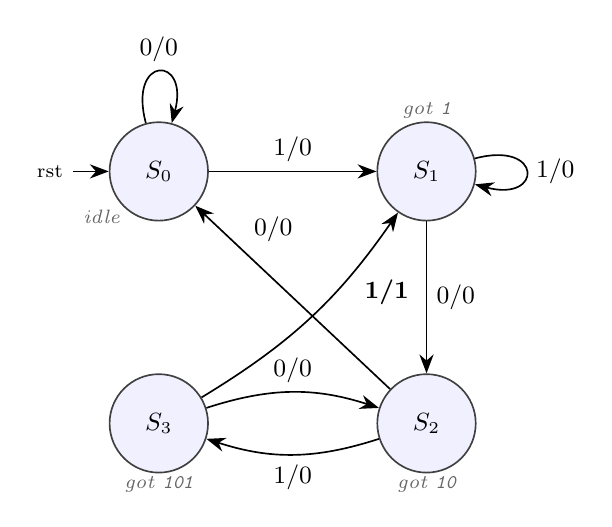
\begin{tikzpicture}[fsm,scale=1.00,transform shape]
\node[state,initial,label={[meaning]below left:{\textit{idle}}}] (S0) at (0.00,0.00) {$S_{0}$};
\node[state,label={[meaning]above:{got \texttt{1}}}] (S1) at (3.40,0.00) {$S_{1}$};
\node[state,label={[meaning]below:{got \texttt{10}}}] (S2) at (3.40,-3.20) {$S_{2}$};
\node[state,label={[meaning]below:{got \texttt{101}}}] (S3) at (0.00,-3.20) {$S_{3}$};
\path (S0) edge[loop above] node[elab] {0/0} (S0);
\path (S0) edge[] node[elab] {1/0} (S1);
\path (S1) edge[loop right] node[elab] {1/0} (S1);
\path (S1) edge[] node[elab] {0/0} (S2);
\path (S2) edge[] node[elab,pos=0.75,swap] {0/0} (S0);
\path (S2) edge[bend left=18] node[elab] {1/0} (S3);
\path (S3) edge[bend left=18] node[elab] {0/0} (S2);
\path (S3) edge[bend right=12] node[elab,pos=0.75,swap] {\textbf{1/1}} (S1);
\end{tikzpicture}
\end{center}
\subsection{Step-by-step}
{\small Legend for the step-by-step pictures: \tikz\node[draw=black!75,fill=yellow!75,circle,minimum size=3mm,inner sep=0]{};~present state \quad \tikz\node[draw=red!80!black,line width=1.6pt,fill=blue!6,circle,minimum size=3mm,inner sep=0]{};~next state \quad \tikz\draw[->,>=Stealth,red!80!black,line width=1.6pt](0,0)--(0.6,0);~transition taken on this clock edge}\par\smallskip\noindent
\begin{minipage}[t]{0.327\textwidth}\centering
\fcolorbox{black!15}{white}{\begin{minipage}{0.94\linewidth}\centering
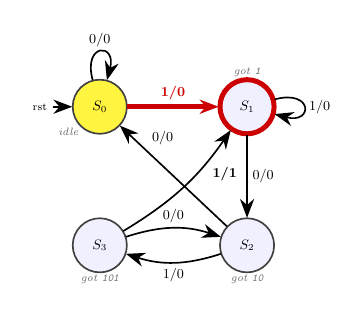
\begin{tikzpicture}[fsm,scale=0.55,transform shape]
\node[state,initial,cur,label={[meaning]below left:{\textit{idle}}}] (S0) at (0.00,0.00) {$S_{0}$};
\node[state,nxt,label={[meaning]above:{got \texttt{1}}}] (S1) at (3.40,0.00) {$S_{1}$};
\node[state,label={[meaning]below:{got \texttt{10}}}] (S2) at (3.40,-3.20) {$S_{2}$};
\node[state,label={[meaning]below:{got \texttt{101}}}] (S3) at (0.00,-3.20) {$S_{3}$};
\path (S0) edge[loop above] node[elab] {0/0} (S0);
\path (S0) edge[hl] node[elab,hlnode] {1/0} (S1);
\path (S1) edge[loop right] node[elab] {1/0} (S1);
\path (S1) edge[] node[elab] {0/0} (S2);
\path (S2) edge[] node[elab,pos=0.75,swap] {0/0} (S0);
\path (S2) edge[bend left=18] node[elab] {1/0} (S3);
\path (S3) edge[bend left=18] node[elab] {0/0} (S2);
\path (S3) edge[bend right=12] node[elab,pos=0.75,swap] {\textbf{1/1}} (S1);
\end{tikzpicture}
\\[2pt]{\small\textbf{Clock 1}: \texttt{serin=1}}\\[1pt]{\scriptsize $S_{0}$ $\rightarrow$ $S_{1}$ \;|\; det\_out=0 {\tiny(before edge)}}\end{minipage}}\end{minipage}
\hfill
\begin{minipage}[t]{0.327\textwidth}\centering
\fcolorbox{black!15}{white}{\begin{minipage}{0.94\linewidth}\centering
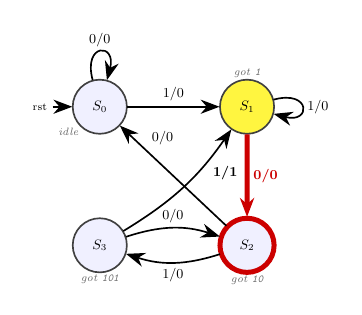
\begin{tikzpicture}[fsm,scale=0.55,transform shape]
\node[state,initial,label={[meaning]below left:{\textit{idle}}}] (S0) at (0.00,0.00) {$S_{0}$};
\node[state,cur,label={[meaning]above:{got \texttt{1}}}] (S1) at (3.40,0.00) {$S_{1}$};
\node[state,nxt,label={[meaning]below:{got \texttt{10}}}] (S2) at (3.40,-3.20) {$S_{2}$};
\node[state,label={[meaning]below:{got \texttt{101}}}] (S3) at (0.00,-3.20) {$S_{3}$};
\path (S0) edge[loop above] node[elab] {0/0} (S0);
\path (S0) edge[] node[elab] {1/0} (S1);
\path (S1) edge[loop right] node[elab] {1/0} (S1);
\path (S1) edge[hl] node[elab,hlnode] {0/0} (S2);
\path (S2) edge[] node[elab,pos=0.75,swap] {0/0} (S0);
\path (S2) edge[bend left=18] node[elab] {1/0} (S3);
\path (S3) edge[bend left=18] node[elab] {0/0} (S2);
\path (S3) edge[bend right=12] node[elab,pos=0.75,swap] {\textbf{1/1}} (S1);
\end{tikzpicture}
\\[2pt]{\small\textbf{Clock 2}: \texttt{serin=0}}\\[1pt]{\scriptsize $S_{1}$ $\rightarrow$ $S_{2}$ \;|\; det\_out=0 {\tiny(before edge)}}\end{minipage}}\end{minipage}
\hfill
\begin{minipage}[t]{0.327\textwidth}\centering
\fcolorbox{black!15}{white}{\begin{minipage}{0.94\linewidth}\centering
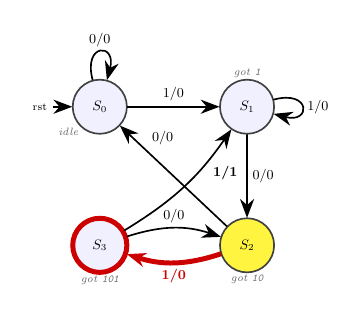
\begin{tikzpicture}[fsm,scale=0.55,transform shape]
\node[state,initial,label={[meaning]below left:{\textit{idle}}}] (S0) at (0.00,0.00) {$S_{0}$};
\node[state,label={[meaning]above:{got \texttt{1}}}] (S1) at (3.40,0.00) {$S_{1}$};
\node[state,cur,label={[meaning]below:{got \texttt{10}}}] (S2) at (3.40,-3.20) {$S_{2}$};
\node[state,nxt,label={[meaning]below:{got \texttt{101}}}] (S3) at (0.00,-3.20) {$S_{3}$};
\path (S0) edge[loop above] node[elab] {0/0} (S0);
\path (S0) edge[] node[elab] {1/0} (S1);
\path (S1) edge[loop right] node[elab] {1/0} (S1);
\path (S1) edge[] node[elab] {0/0} (S2);
\path (S2) edge[] node[elab,pos=0.75,swap] {0/0} (S0);
\path (S2) edge[bend left=18,hl] node[elab,hlnode] {1/0} (S3);
\path (S3) edge[bend left=18] node[elab] {0/0} (S2);
\path (S3) edge[bend right=12] node[elab,pos=0.75,swap] {\textbf{1/1}} (S1);
\end{tikzpicture}
\\[2pt]{\small\textbf{Clock 3}: \texttt{serin=1}}\\[1pt]{\scriptsize $S_{2}$ $\rightarrow$ $S_{3}$ \;|\; det\_out=0 {\tiny(before edge)}}\end{minipage}}\end{minipage}
\par\medskip\noindent
\begin{minipage}[t]{0.327\textwidth}\centering
\fcolorbox{black!15}{white}{\begin{minipage}{0.94\linewidth}\centering
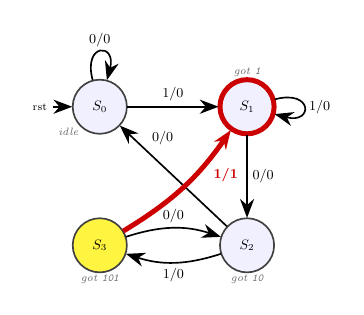
\begin{tikzpicture}[fsm,scale=0.55,transform shape]
\node[state,initial,label={[meaning]below left:{\textit{idle}}}] (S0) at (0.00,0.00) {$S_{0}$};
\node[state,nxt,label={[meaning]above:{got \texttt{1}}}] (S1) at (3.40,0.00) {$S_{1}$};
\node[state,label={[meaning]below:{got \texttt{10}}}] (S2) at (3.40,-3.20) {$S_{2}$};
\node[state,cur,label={[meaning]below:{got \texttt{101}}}] (S3) at (0.00,-3.20) {$S_{3}$};
\path (S0) edge[loop above] node[elab] {0/0} (S0);
\path (S0) edge[] node[elab] {1/0} (S1);
\path (S1) edge[loop right] node[elab] {1/0} (S1);
\path (S1) edge[] node[elab] {0/0} (S2);
\path (S2) edge[] node[elab,pos=0.75,swap] {0/0} (S0);
\path (S2) edge[bend left=18] node[elab] {1/0} (S3);
\path (S3) edge[bend left=18] node[elab] {0/0} (S2);
\path (S3) edge[bend right=12,hl] node[elab,pos=0.75,swap,hlnode] {\textbf{1/1}} (S1);
\end{tikzpicture}
\\[2pt]{\small\textbf{Clock 4}: \texttt{serin=1}}\\[1pt]{\scriptsize $S_{3}$ $\rightarrow$ $S_{1}$ \;|\; \textcolor{red!80!black}{\textbf{det\_out=1}} {\tiny(before edge)}}\end{minipage}}\end{minipage}
\hfill
\begin{minipage}[t]{0.327\textwidth}\centering
\fcolorbox{black!15}{white}{\begin{minipage}{0.94\linewidth}\centering
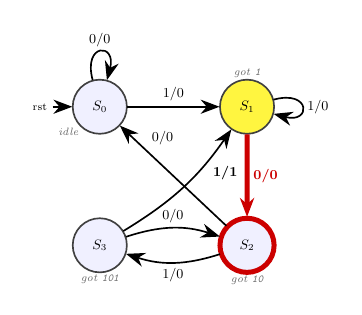
\begin{tikzpicture}[fsm,scale=0.55,transform shape]
\node[state,initial,label={[meaning]below left:{\textit{idle}}}] (S0) at (0.00,0.00) {$S_{0}$};
\node[state,cur,label={[meaning]above:{got \texttt{1}}}] (S1) at (3.40,0.00) {$S_{1}$};
\node[state,nxt,label={[meaning]below:{got \texttt{10}}}] (S2) at (3.40,-3.20) {$S_{2}$};
\node[state,label={[meaning]below:{got \texttt{101}}}] (S3) at (0.00,-3.20) {$S_{3}$};
\path (S0) edge[loop above] node[elab] {0/0} (S0);
\path (S0) edge[] node[elab] {1/0} (S1);
\path (S1) edge[loop right] node[elab] {1/0} (S1);
\path (S1) edge[hl] node[elab,hlnode] {0/0} (S2);
\path (S2) edge[] node[elab,pos=0.75,swap] {0/0} (S0);
\path (S2) edge[bend left=18] node[elab] {1/0} (S3);
\path (S3) edge[bend left=18] node[elab] {0/0} (S2);
\path (S3) edge[bend right=12] node[elab,pos=0.75,swap] {\textbf{1/1}} (S1);
\end{tikzpicture}
\\[2pt]{\small\textbf{Clock 5}: \texttt{serin=0}}\\[1pt]{\scriptsize $S_{1}$ $\rightarrow$ $S_{2}$ \;|\; det\_out=0 {\tiny(before edge)}}\end{minipage}}\end{minipage}
\hfill
\begin{minipage}[t]{0.327\textwidth}\centering
\fcolorbox{black!15}{white}{\begin{minipage}{0.94\linewidth}\centering
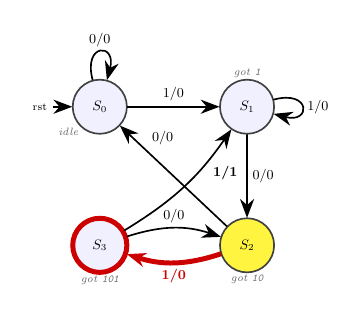
\begin{tikzpicture}[fsm,scale=0.55,transform shape]
\node[state,initial,label={[meaning]below left:{\textit{idle}}}] (S0) at (0.00,0.00) {$S_{0}$};
\node[state,label={[meaning]above:{got \texttt{1}}}] (S1) at (3.40,0.00) {$S_{1}$};
\node[state,cur,label={[meaning]below:{got \texttt{10}}}] (S2) at (3.40,-3.20) {$S_{2}$};
\node[state,nxt,label={[meaning]below:{got \texttt{101}}}] (S3) at (0.00,-3.20) {$S_{3}$};
\path (S0) edge[loop above] node[elab] {0/0} (S0);
\path (S0) edge[] node[elab] {1/0} (S1);
\path (S1) edge[loop right] node[elab] {1/0} (S1);
\path (S1) edge[] node[elab] {0/0} (S2);
\path (S2) edge[] node[elab,pos=0.75,swap] {0/0} (S0);
\path (S2) edge[bend left=18,hl] node[elab,hlnode] {1/0} (S3);
\path (S3) edge[bend left=18] node[elab] {0/0} (S2);
\path (S3) edge[bend right=12] node[elab,pos=0.75,swap] {\textbf{1/1}} (S1);
\end{tikzpicture}
\\[2pt]{\small\textbf{Clock 6}: \texttt{serin=1}}\\[1pt]{\scriptsize $S_{2}$ $\rightarrow$ $S_{3}$ \;|\; det\_out=0 {\tiny(before edge)}}\end{minipage}}\end{minipage}
\par\medskip\noindent
\begin{minipage}[t]{0.327\textwidth}\centering
\fcolorbox{black!15}{white}{\begin{minipage}{0.94\linewidth}\centering
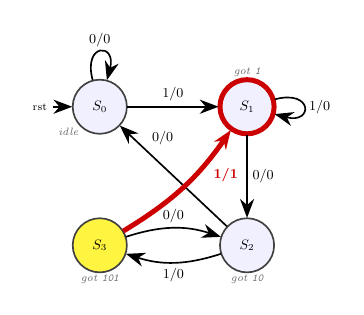
\begin{tikzpicture}[fsm,scale=0.55,transform shape]
\node[state,initial,label={[meaning]below left:{\textit{idle}}}] (S0) at (0.00,0.00) {$S_{0}$};
\node[state,nxt,label={[meaning]above:{got \texttt{1}}}] (S1) at (3.40,0.00) {$S_{1}$};
\node[state,label={[meaning]below:{got \texttt{10}}}] (S2) at (3.40,-3.20) {$S_{2}$};
\node[state,cur,label={[meaning]below:{got \texttt{101}}}] (S3) at (0.00,-3.20) {$S_{3}$};
\path (S0) edge[loop above] node[elab] {0/0} (S0);
\path (S0) edge[] node[elab] {1/0} (S1);
\path (S1) edge[loop right] node[elab] {1/0} (S1);
\path (S1) edge[] node[elab] {0/0} (S2);
\path (S2) edge[] node[elab,pos=0.75,swap] {0/0} (S0);
\path (S2) edge[bend left=18] node[elab] {1/0} (S3);
\path (S3) edge[bend left=18] node[elab] {0/0} (S2);
\path (S3) edge[bend right=12,hl] node[elab,pos=0.75,swap,hlnode] {\textbf{1/1}} (S1);
\end{tikzpicture}
\\[2pt]{\small\textbf{Clock 7}: \texttt{serin=1}}\\[1pt]{\scriptsize $S_{3}$ $\rightarrow$ $S_{1}$ \;|\; \textcolor{red!80!black}{\textbf{det\_out=1}} {\tiny(before edge)}}\end{minipage}}\end{minipage}
\hfill
\begin{minipage}[t]{0.327\textwidth}\centering
\fcolorbox{black!15}{white}{\begin{minipage}{0.94\linewidth}\centering
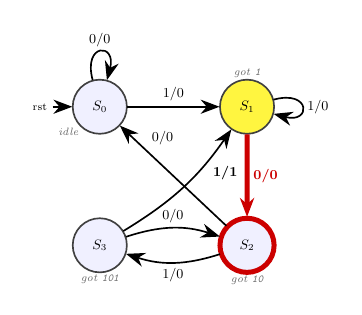
\begin{tikzpicture}[fsm,scale=0.55,transform shape]
\node[state,initial,label={[meaning]below left:{\textit{idle}}}] (S0) at (0.00,0.00) {$S_{0}$};
\node[state,cur,label={[meaning]above:{got \texttt{1}}}] (S1) at (3.40,0.00) {$S_{1}$};
\node[state,nxt,label={[meaning]below:{got \texttt{10}}}] (S2) at (3.40,-3.20) {$S_{2}$};
\node[state,label={[meaning]below:{got \texttt{101}}}] (S3) at (0.00,-3.20) {$S_{3}$};
\path (S0) edge[loop above] node[elab] {0/0} (S0);
\path (S0) edge[] node[elab] {1/0} (S1);
\path (S1) edge[loop right] node[elab] {1/0} (S1);
\path (S1) edge[hl] node[elab,hlnode] {0/0} (S2);
\path (S2) edge[] node[elab,pos=0.75,swap] {0/0} (S0);
\path (S2) edge[bend left=18] node[elab] {1/0} (S3);
\path (S3) edge[bend left=18] node[elab] {0/0} (S2);
\path (S3) edge[bend right=12] node[elab,pos=0.75,swap] {\textbf{1/1}} (S1);
\end{tikzpicture}
\\[2pt]{\small\textbf{Clock 8}: \texttt{serin=0}}\\[1pt]{\scriptsize $S_{1}$ $\rightarrow$ $S_{2}$ \;|\; det\_out=0 {\tiny(before edge)}}\end{minipage}}\end{minipage}
\hfill
\begin{minipage}[t]{0.327\textwidth}\centering
\fcolorbox{black!15}{white}{\begin{minipage}{0.94\linewidth}\centering
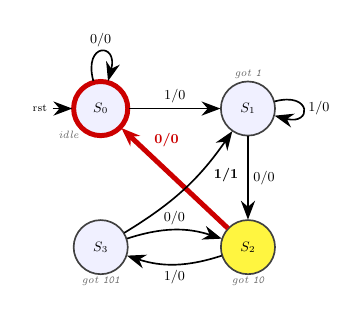
\begin{tikzpicture}[fsm,scale=0.55,transform shape]
\node[state,initial,nxt,label={[meaning]below left:{\textit{idle}}}] (S0) at (0.00,0.00) {$S_{0}$};
\node[state,label={[meaning]above:{got \texttt{1}}}] (S1) at (3.40,0.00) {$S_{1}$};
\node[state,cur,label={[meaning]below:{got \texttt{10}}}] (S2) at (3.40,-3.20) {$S_{2}$};
\node[state,label={[meaning]below:{got \texttt{101}}}] (S3) at (0.00,-3.20) {$S_{3}$};
\path (S0) edge[loop above] node[elab] {0/0} (S0);
\path (S0) edge[] node[elab] {1/0} (S1);
\path (S1) edge[loop right] node[elab] {1/0} (S1);
\path (S1) edge[] node[elab] {0/0} (S2);
\path (S2) edge[hl] node[elab,pos=0.75,swap,hlnode] {0/0} (S0);
\path (S2) edge[bend left=18] node[elab] {1/0} (S3);
\path (S3) edge[bend left=18] node[elab] {0/0} (S2);
\path (S3) edge[bend right=12] node[elab,pos=0.75,swap] {\textbf{1/1}} (S1);
\end{tikzpicture}
\\[2pt]{\small\textbf{Clock 9}: \texttt{serin=0}}\\[1pt]{\scriptsize $S_{2}$ $\rightarrow$ $S_{0}$ \;|\; det\_out=0 {\tiny(before edge)}}\end{minipage}}\end{minipage}
\par\medskip\noindent
\subsection{Trace table and waveform}
\begin{center}\small
\begin{tabular}{c c c c c}
\toprule
Clock edge & \texttt{serin} sampled & Present state & Next state & \texttt{det\_out} {\scriptsize before edge (Mealy)}\\
\midrule
1 & \texttt{1} & $S_{0}$ & $S_{1}$ & 0\\
2 & \texttt{0} & $S_{1}$ & $S_{2}$ & 0\\
3 & \texttt{1} & $S_{2}$ & $S_{3}$ & 0\\
\rowcolor{red!12}4 & \texttt{1} & $S_{3}$ & $S_{1}$ & \textbf{1}\\
5 & \texttt{0} & $S_{1}$ & $S_{2}$ & 0\\
6 & \texttt{1} & $S_{2}$ & $S_{3}$ & 0\\
\rowcolor{red!12}7 & \texttt{1} & $S_{3}$ & $S_{1}$ & \textbf{1}\\
8 & \texttt{0} & $S_{1}$ & $S_{2}$ & 0\\
9 & \texttt{0} & $S_{2}$ & $S_{0}$ & 0\\
10 & \texttt{1} & $S_{0}$ & $S_{1}$ & 0\\
11 & \texttt{0} & $S_{1}$ & $S_{2}$ & 0\\
12 & \texttt{1} & $S_{2}$ & $S_{3}$ & 0\\
13 & \texttt{0} & $S_{3}$ & $S_{2}$ & 0\\
14 & \texttt{1} & $S_{2}$ & $S_{3}$ & 0\\
\bottomrule
\end{tabular}\end{center}\begin{center}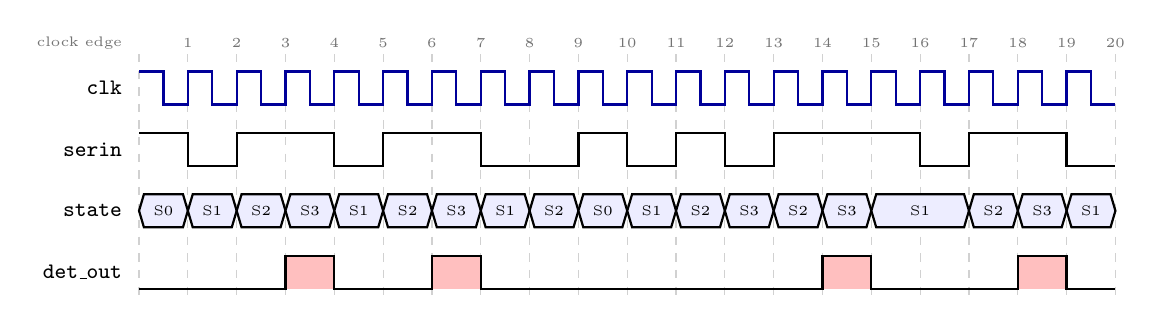
\begin{tikzpicture}[x=0.62cm,y=1cm,font=\scriptsize]
\draw[black!18,dashed] (0,0.64)--(0,-2.44);
\draw[black!18,dashed] (1,0.64)--(1,-2.44);
\node[black!55,font=\tiny] at (1,0.78) {1};
\draw[black!18,dashed] (2,0.64)--(2,-2.44);
\node[black!55,font=\tiny] at (2,0.78) {2};
\draw[black!18,dashed] (3,0.64)--(3,-2.44);
\node[black!55,font=\tiny] at (3,0.78) {3};
\draw[black!18,dashed] (4,0.64)--(4,-2.44);
\node[black!55,font=\tiny] at (4,0.78) {4};
\draw[black!18,dashed] (5,0.64)--(5,-2.44);
\node[black!55,font=\tiny] at (5,0.78) {5};
\draw[black!18,dashed] (6,0.64)--(6,-2.44);
\node[black!55,font=\tiny] at (6,0.78) {6};
\draw[black!18,dashed] (7,0.64)--(7,-2.44);
\node[black!55,font=\tiny] at (7,0.78) {7};
\draw[black!18,dashed] (8,0.64)--(8,-2.44);
\node[black!55,font=\tiny] at (8,0.78) {8};
\draw[black!18,dashed] (9,0.64)--(9,-2.44);
\node[black!55,font=\tiny] at (9,0.78) {9};
\draw[black!18,dashed] (10,0.64)--(10,-2.44);
\node[black!55,font=\tiny] at (10,0.78) {10};
\draw[black!18,dashed] (11,0.64)--(11,-2.44);
\node[black!55,font=\tiny] at (11,0.78) {11};
\draw[black!18,dashed] (12,0.64)--(12,-2.44);
\node[black!55,font=\tiny] at (12,0.78) {12};
\draw[black!18,dashed] (13,0.64)--(13,-2.44);
\node[black!55,font=\tiny] at (13,0.78) {13};
\draw[black!18,dashed] (14,0.64)--(14,-2.44);
\node[black!55,font=\tiny] at (14,0.78) {14};
\draw[black!18,dashed] (15,0.64)--(15,-2.44);
\node[black!55,font=\tiny] at (15,0.78) {15};
\draw[black!18,dashed] (16,0.64)--(16,-2.44);
\node[black!55,font=\tiny] at (16,0.78) {16};
\draw[black!18,dashed] (17,0.64)--(17,-2.44);
\node[black!55,font=\tiny] at (17,0.78) {17};
\draw[black!18,dashed] (18,0.64)--(18,-2.44);
\node[black!55,font=\tiny] at (18,0.78) {18};
\draw[black!18,dashed] (19,0.64)--(19,-2.44);
\node[black!55,font=\tiny] at (19,0.78) {19};
\draw[black!18,dashed] (20,0.64)--(20,-2.44);
\node[black!55,font=\tiny] at (20,0.78) {20};
\node[anchor=east,black!55,font=\tiny] at (-0.15,0.78) {clock edge};
\node[anchor=east,font=\footnotesize\ttfamily] at (-0.15,0.21) {clk};
\draw[thick,blue!60!black] (0.000,0.420) -- (0.500,0.420) -- (0.500,0.000) -- (1.000,0.000) -- (1.000,0.420) -- (1.500,0.420) -- (1.500,0.000) -- (2.000,0.000) -- (2.000,0.420) -- (2.500,0.420) -- (2.500,0.000) -- (3.000,0.000) -- (3.000,0.420) -- (3.500,0.420) -- (3.500,0.000) -- (4.000,0.000) -- (4.000,0.420) -- (4.500,0.420) -- (4.500,0.000) -- (5.000,0.000) -- (5.000,0.420) -- (5.500,0.420) -- (5.500,0.000) -- (6.000,0.000) -- (6.000,0.420) -- (6.500,0.420) -- (6.500,0.000) -- (7.000,0.000) -- (7.000,0.420) -- (7.500,0.420) -- (7.500,0.000) -- (8.000,0.000) -- (8.000,0.420) -- (8.500,0.420) -- (8.500,0.000) -- (9.000,0.000) -- (9.000,0.420) -- (9.500,0.420) -- (9.500,0.000) -- (10.000,0.000) -- (10.000,0.420) -- (10.500,0.420) -- (10.500,0.000) -- (11.000,0.000) -- (11.000,0.420) -- (11.500,0.420) -- (11.500,0.000) -- (12.000,0.000) -- (12.000,0.420) -- (12.500,0.420) -- (12.500,0.000) -- (13.000,0.000) -- (13.000,0.420) -- (13.500,0.420) -- (13.500,0.000) -- (14.000,0.000) -- (14.000,0.420) -- (14.500,0.420) -- (14.500,0.000) -- (15.000,0.000) -- (15.000,0.420) -- (15.500,0.420) -- (15.500,0.000) -- (16.000,0.000) -- (16.000,0.420) -- (16.500,0.420) -- (16.500,0.000) -- (17.000,0.000) -- (17.000,0.420) -- (17.500,0.420) -- (17.500,0.000) -- (18.000,0.000) -- (18.000,0.420) -- (18.500,0.420) -- (18.500,0.000) -- (19.000,0.000) -- (19.000,0.420) -- (19.500,0.420) -- (19.500,0.000) -- (20.000,0.000);
\node[anchor=east,font=\footnotesize\ttfamily] at (-0.15,-0.57) {serin};
\draw[thick,black] (0.000,-0.360) -- (1.000,-0.360) -- (1.000,-0.780) -- (2.000,-0.780) -- (2.000,-0.360) -- (3.000,-0.360) -- (3.000,-0.360) -- (4.000,-0.360) -- (4.000,-0.780) -- (5.000,-0.780) -- (5.000,-0.360) -- (6.000,-0.360) -- (6.000,-0.360) -- (7.000,-0.360) -- (7.000,-0.780) -- (8.000,-0.780) -- (8.000,-0.780) -- (9.000,-0.780) -- (9.000,-0.360) -- (10.000,-0.360) -- (10.000,-0.780) -- (11.000,-0.780) -- (11.000,-0.360) -- (12.000,-0.360) -- (12.000,-0.780) -- (13.000,-0.780) -- (13.000,-0.360) -- (14.000,-0.360) -- (14.000,-0.360) -- (15.000,-0.360) -- (15.000,-0.360) -- (16.000,-0.360) -- (16.000,-0.780) -- (17.000,-0.780) -- (17.000,-0.360) -- (18.000,-0.360) -- (18.000,-0.360) -- (19.000,-0.360) -- (19.000,-0.780) -- (20.000,-0.780);
\node[anchor=east,font=\footnotesize\ttfamily] at (-0.15,-1.35) {state};
\draw[thick,fill=blue!7] (0.000,-1.350)--(0.100,-1.140)--(0.900,-1.140)--(1.000,-1.350)--(0.900,-1.560)--(0.100,-1.560)--cycle;
\node[font=\tiny] at (0.500,-1.350) {S0};
\draw[thick,fill=blue!7] (1.000,-1.350)--(1.100,-1.140)--(1.900,-1.140)--(2.000,-1.350)--(1.900,-1.560)--(1.100,-1.560)--cycle;
\node[font=\tiny] at (1.500,-1.350) {S1};
\draw[thick,fill=blue!7] (2.000,-1.350)--(2.100,-1.140)--(2.900,-1.140)--(3.000,-1.350)--(2.900,-1.560)--(2.100,-1.560)--cycle;
\node[font=\tiny] at (2.500,-1.350) {S2};
\draw[thick,fill=blue!7] (3.000,-1.350)--(3.100,-1.140)--(3.900,-1.140)--(4.000,-1.350)--(3.900,-1.560)--(3.100,-1.560)--cycle;
\node[font=\tiny] at (3.500,-1.350) {S3};
\draw[thick,fill=blue!7] (4.000,-1.350)--(4.100,-1.140)--(4.900,-1.140)--(5.000,-1.350)--(4.900,-1.560)--(4.100,-1.560)--cycle;
\node[font=\tiny] at (4.500,-1.350) {S1};
\draw[thick,fill=blue!7] (5.000,-1.350)--(5.100,-1.140)--(5.900,-1.140)--(6.000,-1.350)--(5.900,-1.560)--(5.100,-1.560)--cycle;
\node[font=\tiny] at (5.500,-1.350) {S2};
\draw[thick,fill=blue!7] (6.000,-1.350)--(6.100,-1.140)--(6.900,-1.140)--(7.000,-1.350)--(6.900,-1.560)--(6.100,-1.560)--cycle;
\node[font=\tiny] at (6.500,-1.350) {S3};
\draw[thick,fill=blue!7] (7.000,-1.350)--(7.100,-1.140)--(7.900,-1.140)--(8.000,-1.350)--(7.900,-1.560)--(7.100,-1.560)--cycle;
\node[font=\tiny] at (7.500,-1.350) {S1};
\draw[thick,fill=blue!7] (8.000,-1.350)--(8.100,-1.140)--(8.900,-1.140)--(9.000,-1.350)--(8.900,-1.560)--(8.100,-1.560)--cycle;
\node[font=\tiny] at (8.500,-1.350) {S2};
\draw[thick,fill=blue!7] (9.000,-1.350)--(9.100,-1.140)--(9.900,-1.140)--(10.000,-1.350)--(9.900,-1.560)--(9.100,-1.560)--cycle;
\node[font=\tiny] at (9.500,-1.350) {S0};
\draw[thick,fill=blue!7] (10.000,-1.350)--(10.100,-1.140)--(10.900,-1.140)--(11.000,-1.350)--(10.900,-1.560)--(10.100,-1.560)--cycle;
\node[font=\tiny] at (10.500,-1.350) {S1};
\draw[thick,fill=blue!7] (11.000,-1.350)--(11.100,-1.140)--(11.900,-1.140)--(12.000,-1.350)--(11.900,-1.560)--(11.100,-1.560)--cycle;
\node[font=\tiny] at (11.500,-1.350) {S2};
\draw[thick,fill=blue!7] (12.000,-1.350)--(12.100,-1.140)--(12.900,-1.140)--(13.000,-1.350)--(12.900,-1.560)--(12.100,-1.560)--cycle;
\node[font=\tiny] at (12.500,-1.350) {S3};
\draw[thick,fill=blue!7] (13.000,-1.350)--(13.100,-1.140)--(13.900,-1.140)--(14.000,-1.350)--(13.900,-1.560)--(13.100,-1.560)--cycle;
\node[font=\tiny] at (13.500,-1.350) {S2};
\draw[thick,fill=blue!7] (14.000,-1.350)--(14.100,-1.140)--(14.900,-1.140)--(15.000,-1.350)--(14.900,-1.560)--(14.100,-1.560)--cycle;
\node[font=\tiny] at (14.500,-1.350) {S3};
\draw[thick,fill=blue!7] (15.000,-1.350)--(15.100,-1.140)--(16.900,-1.140)--(17.000,-1.350)--(16.900,-1.560)--(15.100,-1.560)--cycle;
\node[font=\tiny] at (16.000,-1.350) {S1};
\draw[thick,fill=blue!7] (17.000,-1.350)--(17.100,-1.140)--(17.900,-1.140)--(18.000,-1.350)--(17.900,-1.560)--(17.100,-1.560)--cycle;
\node[font=\tiny] at (17.500,-1.350) {S2};
\draw[thick,fill=blue!7] (18.000,-1.350)--(18.100,-1.140)--(18.900,-1.140)--(19.000,-1.350)--(18.900,-1.560)--(18.100,-1.560)--cycle;
\node[font=\tiny] at (18.500,-1.350) {S3};
\draw[thick,fill=blue!7] (19.000,-1.350)--(19.100,-1.140)--(19.900,-1.140)--(20.000,-1.350)--(19.900,-1.560)--(19.100,-1.560)--cycle;
\node[font=\tiny] at (19.500,-1.350) {S1};
\node[anchor=east,font=\footnotesize\ttfamily] at (-0.15,-2.13) {det\_out};
\fill[red!25] (3.000,-2.340) rectangle (4.000,-1.920);
\fill[red!25] (6.000,-2.340) rectangle (7.000,-1.920);
\fill[red!25] (14.000,-2.340) rectangle (15.000,-1.920);
\fill[red!25] (18.000,-2.340) rectangle (19.000,-1.920);
\draw[thick,black] (0.000,-2.340) -- (1.000,-2.340) -- (1.000,-2.340) -- (2.000,-2.340) -- (2.000,-2.340) -- (3.000,-2.340) -- (3.000,-1.920) -- (4.000,-1.920) -- (4.000,-2.340) -- (5.000,-2.340) -- (5.000,-2.340) -- (6.000,-2.340) -- (6.000,-1.920) -- (7.000,-1.920) -- (7.000,-2.340) -- (8.000,-2.340) -- (8.000,-2.340) -- (9.000,-2.340) -- (9.000,-2.340) -- (10.000,-2.340) -- (10.000,-2.340) -- (11.000,-2.340) -- (11.000,-2.340) -- (12.000,-2.340) -- (12.000,-2.340) -- (13.000,-2.340) -- (13.000,-2.340) -- (14.000,-2.340) -- (14.000,-1.920) -- (15.000,-1.920) -- (15.000,-2.340) -- (16.000,-2.340) -- (16.000,-2.340) -- (17.000,-2.340) -- (17.000,-2.340) -- (18.000,-2.340) -- (18.000,-1.920) -- (19.000,-1.920) -- (19.000,-2.340) -- (20.000,-2.340);
\end{tikzpicture}\end{center}
{\small Mealy: \texttt{det\_out} is high \emph{during} the clock in which the final 1 is on the input,
so it is captured by the same edge that samples that bit. Clocks 4 and 7 show the overlap:
``1011011'' gives two hits.}

\begin{codeslice}{RTL -- \texttt{1011} overlapping, Mealy}{seq1011\_mealy.v}
\slicenote{In \texttt{S3} the 1 that completes the pattern is also the start of the next one, so go to \texttt{S1}, not \texttt{S0}.}
\begin{lstlisting}
`timescale 1ns/1ps
// Overlapping "1011" detector -- Mealy FSM
module seq1011_mealy (
    input  wire clk,
    input  wire rst,
    input  wire serin,
    output reg  det_out
);
    localparam [1:0] S0 = 2'd0,   // idle
                     S1 = 2'd1,   // got "1"
                     S2 = 2'd2,   // got "10"
                     S3 = 2'd3;   // got "101"
    reg [1:0] state, next_state;

    always @(posedge clk or posedge rst)
        if (rst) state <= S0;
        else     state <= next_state;

    always @(*) begin
        next_state = S0;
        det_out    = 1'b0;
        case (state)
            S0: next_state = serin ? S1 : S0;
            S1: next_state = serin ? S1 : S2;   // "11" -> still "1"
            S2: next_state = serin ? S3 : S0;   // "100" -> nothing
            S3: if (serin) begin                // "1011" found!
                    next_state = S1;            // overlap: keep last "1"
                    det_out    = 1'b1;
                end else
                    next_state = S2;            // "1010" -> keep "10"
            default: next_state = S0;
        endcase
    end
endmodule
\end{lstlisting}
\end{codeslice}\begin{codeslice}{TB -- Mealy output is checked just before the clock edge}{tb\_seq1011.v}
\slicenote{For a Mealy FSM, sample \texttt{det\_out} at the rising edge with \texttt{\$display} (old state, current input). Do not use \texttt{\$strobe} here.}
\begin{lstlisting}
`timescale 1ns/1ps
module tb_seq1011;
    reg  clk = 1'b0, rst = 1'b1, serin = 1'b0;
    wire det_out;
    integer i, hits = 0;

    seq1011_mealy dut (.clk(clk), .rst(rst), .serin(serin), .det_out(det_out));

    always #5 clk = ~clk;

    initial begin
        $dumpfile("tb_seq1011.vcd");
        $dumpvars(0, tb_seq1011);
        repeat (2) @(posedge clk);
        #1 rst = 1'b0;
        for (i = 0; i < 100; i = i + 1) begin
            serin = $random;
            @(posedge clk); #1;
        end
        $display("DONE: %0d detections of 1011", hits);
        $finish;
    end

    always @(posedge clk)                    // values just BEFORE the edge
        if (!rst) begin
            $display("%6t  state=S%0d  serin=%b  det_out=%b",
                     $time, dut.state, serin, det_out);
            if (det_out) hits = hits + 1;
        end
endmodule
\end{lstlisting}
\end{codeslice}


\newpage
\section{Predicted P4 -- ``101'': overlapping vs.\ non-overlapping (Moore)}
\begin{qbox}{Likely wording}
Design a Moore FSM to detect ``101''. (a) overlapping, (b) non-overlapping. Compare the outputs for the same
input stream.
\end{qbox}
\begin{center}
\begin{minipage}{0.48\textwidth}\centering\textbf{(a) Overlapping}\\[2pt]
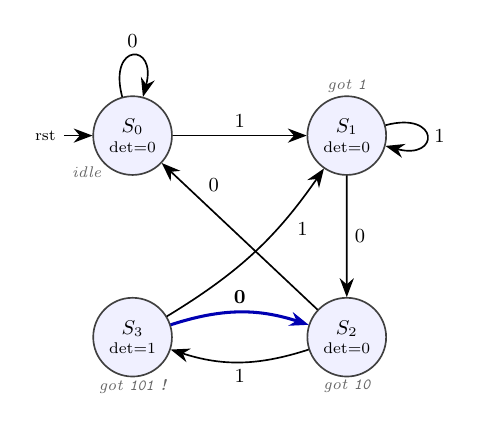
\begin{tikzpicture}[fsm,scale=0.80,transform shape]
\node[state,initial,label={[meaning]below left:{\textit{idle}}}] (S0) at (0.00,0.00) {$S_{0}$\\[-2pt]{\scriptsize det=0}};
\node[state,label={[meaning]above:{got \texttt{1}}}] (S1) at (3.40,0.00) {$S_{1}$\\[-2pt]{\scriptsize det=0}};
\node[state,label={[meaning]below:{got \texttt{10}}}] (S2) at (3.40,-3.20) {$S_{2}$\\[-2pt]{\scriptsize det=0}};
\node[state,label={[meaning]below:{got \texttt{101} \textbf{!}}}] (S3) at (0.00,-3.20) {$S_{3}$\\[-2pt]{\scriptsize det=1}};
\path (S0) edge[loop above] node[elab] {0} (S0);
\path (S0) edge[] node[elab] {1} (S1);
\path (S1) edge[loop right] node[elab] {1} (S1);
\path (S1) edge[] node[elab] {0} (S2);
\path (S2) edge[] node[elab,pos=0.75,swap] {0} (S0);
\path (S2) edge[bend left=18] node[elab] {1} (S3);
\path (S3) edge[bend right=12] node[elab,pos=0.75,swap] {1} (S1);
\path (S3) edge[bend left=18,hlx] node[elab] {\textbf{0}} (S2);
\end{tikzpicture}
\end{minipage}\hfill
\begin{minipage}{0.48\textwidth}\centering\textbf{(b) Non-overlapping}\\[2pt]
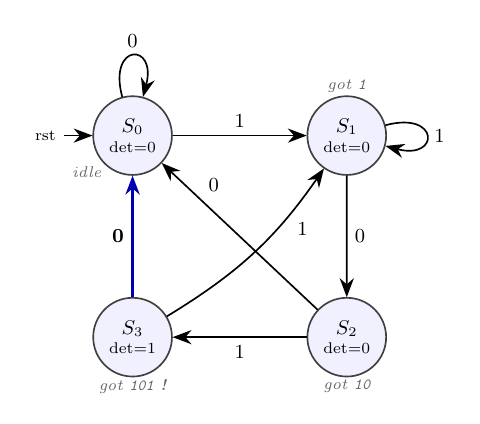
\begin{tikzpicture}[fsm,scale=0.80,transform shape]
\node[state,initial,label={[meaning]below left:{\textit{idle}}}] (S0) at (0.00,0.00) {$S_{0}$\\[-2pt]{\scriptsize det=0}};
\node[state,label={[meaning]above:{got \texttt{1}}}] (S1) at (3.40,0.00) {$S_{1}$\\[-2pt]{\scriptsize det=0}};
\node[state,label={[meaning]below:{got \texttt{10}}}] (S2) at (3.40,-3.20) {$S_{2}$\\[-2pt]{\scriptsize det=0}};
\node[state,label={[meaning]below:{got \texttt{101} \textbf{!}}}] (S3) at (0.00,-3.20) {$S_{3}$\\[-2pt]{\scriptsize det=1}};
\path (S0) edge[loop above] node[elab] {0} (S0);
\path (S0) edge[] node[elab] {1} (S1);
\path (S1) edge[loop right] node[elab] {1} (S1);
\path (S1) edge[] node[elab] {0} (S2);
\path (S2) edge[] node[elab,pos=0.75,swap] {0} (S0);
\path (S2) edge[] node[elab] {1} (S3);
\path (S3) edge[bend right=12] node[elab,pos=0.75,swap] {1} (S1);
\path (S3) edge[hlx] node[elab] {\textbf{0}} (S0);
\end{tikzpicture}
\end{minipage}
\end{center}
{\small The \textcolor{blue!70!black}{blue} arrow is the only difference. With overlap, in $S_3$ (``101'') a 0 gives ``1010'', whose
ending ``10'' is reused, so go to $S_2$. Without overlap, the bits are used up, so go to $S_0$.}

\subsection{Waveform: same input, both machines}
\begin{center}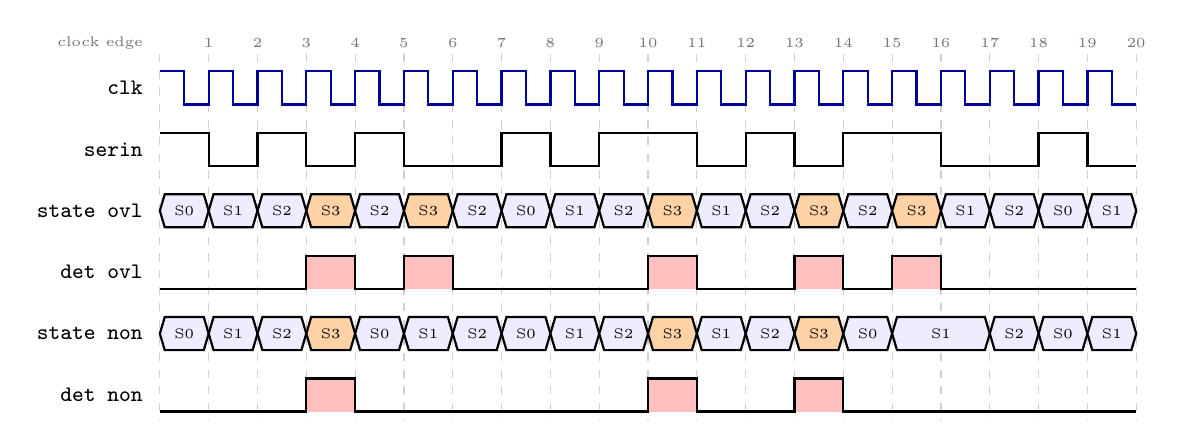
\begin{tikzpicture}[x=0.62cm,y=1cm,font=\scriptsize]
\draw[black!18,dashed] (0,0.64)--(0,-4.00);
\draw[black!18,dashed] (1,0.64)--(1,-4.00);
\node[black!55,font=\tiny] at (1,0.78) {1};
\draw[black!18,dashed] (2,0.64)--(2,-4.00);
\node[black!55,font=\tiny] at (2,0.78) {2};
\draw[black!18,dashed] (3,0.64)--(3,-4.00);
\node[black!55,font=\tiny] at (3,0.78) {3};
\draw[black!18,dashed] (4,0.64)--(4,-4.00);
\node[black!55,font=\tiny] at (4,0.78) {4};
\draw[black!18,dashed] (5,0.64)--(5,-4.00);
\node[black!55,font=\tiny] at (5,0.78) {5};
\draw[black!18,dashed] (6,0.64)--(6,-4.00);
\node[black!55,font=\tiny] at (6,0.78) {6};
\draw[black!18,dashed] (7,0.64)--(7,-4.00);
\node[black!55,font=\tiny] at (7,0.78) {7};
\draw[black!18,dashed] (8,0.64)--(8,-4.00);
\node[black!55,font=\tiny] at (8,0.78) {8};
\draw[black!18,dashed] (9,0.64)--(9,-4.00);
\node[black!55,font=\tiny] at (9,0.78) {9};
\draw[black!18,dashed] (10,0.64)--(10,-4.00);
\node[black!55,font=\tiny] at (10,0.78) {10};
\draw[black!18,dashed] (11,0.64)--(11,-4.00);
\node[black!55,font=\tiny] at (11,0.78) {11};
\draw[black!18,dashed] (12,0.64)--(12,-4.00);
\node[black!55,font=\tiny] at (12,0.78) {12};
\draw[black!18,dashed] (13,0.64)--(13,-4.00);
\node[black!55,font=\tiny] at (13,0.78) {13};
\draw[black!18,dashed] (14,0.64)--(14,-4.00);
\node[black!55,font=\tiny] at (14,0.78) {14};
\draw[black!18,dashed] (15,0.64)--(15,-4.00);
\node[black!55,font=\tiny] at (15,0.78) {15};
\draw[black!18,dashed] (16,0.64)--(16,-4.00);
\node[black!55,font=\tiny] at (16,0.78) {16};
\draw[black!18,dashed] (17,0.64)--(17,-4.00);
\node[black!55,font=\tiny] at (17,0.78) {17};
\draw[black!18,dashed] (18,0.64)--(18,-4.00);
\node[black!55,font=\tiny] at (18,0.78) {18};
\draw[black!18,dashed] (19,0.64)--(19,-4.00);
\node[black!55,font=\tiny] at (19,0.78) {19};
\draw[black!18,dashed] (20,0.64)--(20,-4.00);
\node[black!55,font=\tiny] at (20,0.78) {20};
\node[anchor=east,black!55,font=\tiny] at (-0.15,0.78) {clock edge};
\node[anchor=east,font=\footnotesize\ttfamily] at (-0.15,0.21) {clk};
\draw[thick,blue!60!black] (0.000,0.420) -- (0.500,0.420) -- (0.500,0.000) -- (1.000,0.000) -- (1.000,0.420) -- (1.500,0.420) -- (1.500,0.000) -- (2.000,0.000) -- (2.000,0.420) -- (2.500,0.420) -- (2.500,0.000) -- (3.000,0.000) -- (3.000,0.420) -- (3.500,0.420) -- (3.500,0.000) -- (4.000,0.000) -- (4.000,0.420) -- (4.500,0.420) -- (4.500,0.000) -- (5.000,0.000) -- (5.000,0.420) -- (5.500,0.420) -- (5.500,0.000) -- (6.000,0.000) -- (6.000,0.420) -- (6.500,0.420) -- (6.500,0.000) -- (7.000,0.000) -- (7.000,0.420) -- (7.500,0.420) -- (7.500,0.000) -- (8.000,0.000) -- (8.000,0.420) -- (8.500,0.420) -- (8.500,0.000) -- (9.000,0.000) -- (9.000,0.420) -- (9.500,0.420) -- (9.500,0.000) -- (10.000,0.000) -- (10.000,0.420) -- (10.500,0.420) -- (10.500,0.000) -- (11.000,0.000) -- (11.000,0.420) -- (11.500,0.420) -- (11.500,0.000) -- (12.000,0.000) -- (12.000,0.420) -- (12.500,0.420) -- (12.500,0.000) -- (13.000,0.000) -- (13.000,0.420) -- (13.500,0.420) -- (13.500,0.000) -- (14.000,0.000) -- (14.000,0.420) -- (14.500,0.420) -- (14.500,0.000) -- (15.000,0.000) -- (15.000,0.420) -- (15.500,0.420) -- (15.500,0.000) -- (16.000,0.000) -- (16.000,0.420) -- (16.500,0.420) -- (16.500,0.000) -- (17.000,0.000) -- (17.000,0.420) -- (17.500,0.420) -- (17.500,0.000) -- (18.000,0.000) -- (18.000,0.420) -- (18.500,0.420) -- (18.500,0.000) -- (19.000,0.000) -- (19.000,0.420) -- (19.500,0.420) -- (19.500,0.000) -- (20.000,0.000);
\node[anchor=east,font=\footnotesize\ttfamily] at (-0.15,-0.57) {serin};
\draw[thick,black] (0.000,-0.360) -- (1.000,-0.360) -- (1.000,-0.780) -- (2.000,-0.780) -- (2.000,-0.360) -- (3.000,-0.360) -- (3.000,-0.780) -- (4.000,-0.780) -- (4.000,-0.360) -- (5.000,-0.360) -- (5.000,-0.780) -- (6.000,-0.780) -- (6.000,-0.780) -- (7.000,-0.780) -- (7.000,-0.360) -- (8.000,-0.360) -- (8.000,-0.780) -- (9.000,-0.780) -- (9.000,-0.360) -- (10.000,-0.360) -- (10.000,-0.360) -- (11.000,-0.360) -- (11.000,-0.780) -- (12.000,-0.780) -- (12.000,-0.360) -- (13.000,-0.360) -- (13.000,-0.780) -- (14.000,-0.780) -- (14.000,-0.360) -- (15.000,-0.360) -- (15.000,-0.360) -- (16.000,-0.360) -- (16.000,-0.780) -- (17.000,-0.780) -- (17.000,-0.780) -- (18.000,-0.780) -- (18.000,-0.360) -- (19.000,-0.360) -- (19.000,-0.780) -- (20.000,-0.780);
\node[anchor=east,font=\footnotesize\ttfamily] at (-0.15,-1.35) {state ovl};
\draw[thick,fill=blue!7] (0.000,-1.350)--(0.100,-1.140)--(0.900,-1.140)--(1.000,-1.350)--(0.900,-1.560)--(0.100,-1.560)--cycle;
\node[font=\tiny] at (0.500,-1.350) {S0};
\draw[thick,fill=blue!7] (1.000,-1.350)--(1.100,-1.140)--(1.900,-1.140)--(2.000,-1.350)--(1.900,-1.560)--(1.100,-1.560)--cycle;
\node[font=\tiny] at (1.500,-1.350) {S1};
\draw[thick,fill=blue!7] (2.000,-1.350)--(2.100,-1.140)--(2.900,-1.140)--(3.000,-1.350)--(2.900,-1.560)--(2.100,-1.560)--cycle;
\node[font=\tiny] at (2.500,-1.350) {S2};
\draw[thick,fill=orange!35] (3.000,-1.350)--(3.100,-1.140)--(3.900,-1.140)--(4.000,-1.350)--(3.900,-1.560)--(3.100,-1.560)--cycle;
\node[font=\tiny] at (3.500,-1.350) {S3};
\draw[thick,fill=blue!7] (4.000,-1.350)--(4.100,-1.140)--(4.900,-1.140)--(5.000,-1.350)--(4.900,-1.560)--(4.100,-1.560)--cycle;
\node[font=\tiny] at (4.500,-1.350) {S2};
\draw[thick,fill=orange!35] (5.000,-1.350)--(5.100,-1.140)--(5.900,-1.140)--(6.000,-1.350)--(5.900,-1.560)--(5.100,-1.560)--cycle;
\node[font=\tiny] at (5.500,-1.350) {S3};
\draw[thick,fill=blue!7] (6.000,-1.350)--(6.100,-1.140)--(6.900,-1.140)--(7.000,-1.350)--(6.900,-1.560)--(6.100,-1.560)--cycle;
\node[font=\tiny] at (6.500,-1.350) {S2};
\draw[thick,fill=blue!7] (7.000,-1.350)--(7.100,-1.140)--(7.900,-1.140)--(8.000,-1.350)--(7.900,-1.560)--(7.100,-1.560)--cycle;
\node[font=\tiny] at (7.500,-1.350) {S0};
\draw[thick,fill=blue!7] (8.000,-1.350)--(8.100,-1.140)--(8.900,-1.140)--(9.000,-1.350)--(8.900,-1.560)--(8.100,-1.560)--cycle;
\node[font=\tiny] at (8.500,-1.350) {S1};
\draw[thick,fill=blue!7] (9.000,-1.350)--(9.100,-1.140)--(9.900,-1.140)--(10.000,-1.350)--(9.900,-1.560)--(9.100,-1.560)--cycle;
\node[font=\tiny] at (9.500,-1.350) {S2};
\draw[thick,fill=orange!35] (10.000,-1.350)--(10.100,-1.140)--(10.900,-1.140)--(11.000,-1.350)--(10.900,-1.560)--(10.100,-1.560)--cycle;
\node[font=\tiny] at (10.500,-1.350) {S3};
\draw[thick,fill=blue!7] (11.000,-1.350)--(11.100,-1.140)--(11.900,-1.140)--(12.000,-1.350)--(11.900,-1.560)--(11.100,-1.560)--cycle;
\node[font=\tiny] at (11.500,-1.350) {S1};
\draw[thick,fill=blue!7] (12.000,-1.350)--(12.100,-1.140)--(12.900,-1.140)--(13.000,-1.350)--(12.900,-1.560)--(12.100,-1.560)--cycle;
\node[font=\tiny] at (12.500,-1.350) {S2};
\draw[thick,fill=orange!35] (13.000,-1.350)--(13.100,-1.140)--(13.900,-1.140)--(14.000,-1.350)--(13.900,-1.560)--(13.100,-1.560)--cycle;
\node[font=\tiny] at (13.500,-1.350) {S3};
\draw[thick,fill=blue!7] (14.000,-1.350)--(14.100,-1.140)--(14.900,-1.140)--(15.000,-1.350)--(14.900,-1.560)--(14.100,-1.560)--cycle;
\node[font=\tiny] at (14.500,-1.350) {S2};
\draw[thick,fill=orange!35] (15.000,-1.350)--(15.100,-1.140)--(15.900,-1.140)--(16.000,-1.350)--(15.900,-1.560)--(15.100,-1.560)--cycle;
\node[font=\tiny] at (15.500,-1.350) {S3};
\draw[thick,fill=blue!7] (16.000,-1.350)--(16.100,-1.140)--(16.900,-1.140)--(17.000,-1.350)--(16.900,-1.560)--(16.100,-1.560)--cycle;
\node[font=\tiny] at (16.500,-1.350) {S1};
\draw[thick,fill=blue!7] (17.000,-1.350)--(17.100,-1.140)--(17.900,-1.140)--(18.000,-1.350)--(17.900,-1.560)--(17.100,-1.560)--cycle;
\node[font=\tiny] at (17.500,-1.350) {S2};
\draw[thick,fill=blue!7] (18.000,-1.350)--(18.100,-1.140)--(18.900,-1.140)--(19.000,-1.350)--(18.900,-1.560)--(18.100,-1.560)--cycle;
\node[font=\tiny] at (18.500,-1.350) {S0};
\draw[thick,fill=blue!7] (19.000,-1.350)--(19.100,-1.140)--(19.900,-1.140)--(20.000,-1.350)--(19.900,-1.560)--(19.100,-1.560)--cycle;
\node[font=\tiny] at (19.500,-1.350) {S1};
\node[anchor=east,font=\footnotesize\ttfamily] at (-0.15,-2.13) {det ovl};
\fill[red!25] (3.000,-2.340) rectangle (4.000,-1.920);
\fill[red!25] (5.000,-2.340) rectangle (6.000,-1.920);
\fill[red!25] (10.000,-2.340) rectangle (11.000,-1.920);
\fill[red!25] (13.000,-2.340) rectangle (14.000,-1.920);
\fill[red!25] (15.000,-2.340) rectangle (16.000,-1.920);
\draw[thick,black] (0.000,-2.340) -- (1.000,-2.340) -- (1.000,-2.340) -- (2.000,-2.340) -- (2.000,-2.340) -- (3.000,-2.340) -- (3.000,-1.920) -- (4.000,-1.920) -- (4.000,-2.340) -- (5.000,-2.340) -- (5.000,-1.920) -- (6.000,-1.920) -- (6.000,-2.340) -- (7.000,-2.340) -- (7.000,-2.340) -- (8.000,-2.340) -- (8.000,-2.340) -- (9.000,-2.340) -- (9.000,-2.340) -- (10.000,-2.340) -- (10.000,-1.920) -- (11.000,-1.920) -- (11.000,-2.340) -- (12.000,-2.340) -- (12.000,-2.340) -- (13.000,-2.340) -- (13.000,-1.920) -- (14.000,-1.920) -- (14.000,-2.340) -- (15.000,-2.340) -- (15.000,-1.920) -- (16.000,-1.920) -- (16.000,-2.340) -- (17.000,-2.340) -- (17.000,-2.340) -- (18.000,-2.340) -- (18.000,-2.340) -- (19.000,-2.340) -- (19.000,-2.340) -- (20.000,-2.340);
\node[anchor=east,font=\footnotesize\ttfamily] at (-0.15,-2.91) {state non};
\draw[thick,fill=blue!7] (0.000,-2.910)--(0.100,-2.700)--(0.900,-2.700)--(1.000,-2.910)--(0.900,-3.120)--(0.100,-3.120)--cycle;
\node[font=\tiny] at (0.500,-2.910) {S0};
\draw[thick,fill=blue!7] (1.000,-2.910)--(1.100,-2.700)--(1.900,-2.700)--(2.000,-2.910)--(1.900,-3.120)--(1.100,-3.120)--cycle;
\node[font=\tiny] at (1.500,-2.910) {S1};
\draw[thick,fill=blue!7] (2.000,-2.910)--(2.100,-2.700)--(2.900,-2.700)--(3.000,-2.910)--(2.900,-3.120)--(2.100,-3.120)--cycle;
\node[font=\tiny] at (2.500,-2.910) {S2};
\draw[thick,fill=orange!35] (3.000,-2.910)--(3.100,-2.700)--(3.900,-2.700)--(4.000,-2.910)--(3.900,-3.120)--(3.100,-3.120)--cycle;
\node[font=\tiny] at (3.500,-2.910) {S3};
\draw[thick,fill=blue!7] (4.000,-2.910)--(4.100,-2.700)--(4.900,-2.700)--(5.000,-2.910)--(4.900,-3.120)--(4.100,-3.120)--cycle;
\node[font=\tiny] at (4.500,-2.910) {S0};
\draw[thick,fill=blue!7] (5.000,-2.910)--(5.100,-2.700)--(5.900,-2.700)--(6.000,-2.910)--(5.900,-3.120)--(5.100,-3.120)--cycle;
\node[font=\tiny] at (5.500,-2.910) {S1};
\draw[thick,fill=blue!7] (6.000,-2.910)--(6.100,-2.700)--(6.900,-2.700)--(7.000,-2.910)--(6.900,-3.120)--(6.100,-3.120)--cycle;
\node[font=\tiny] at (6.500,-2.910) {S2};
\draw[thick,fill=blue!7] (7.000,-2.910)--(7.100,-2.700)--(7.900,-2.700)--(8.000,-2.910)--(7.900,-3.120)--(7.100,-3.120)--cycle;
\node[font=\tiny] at (7.500,-2.910) {S0};
\draw[thick,fill=blue!7] (8.000,-2.910)--(8.100,-2.700)--(8.900,-2.700)--(9.000,-2.910)--(8.900,-3.120)--(8.100,-3.120)--cycle;
\node[font=\tiny] at (8.500,-2.910) {S1};
\draw[thick,fill=blue!7] (9.000,-2.910)--(9.100,-2.700)--(9.900,-2.700)--(10.000,-2.910)--(9.900,-3.120)--(9.100,-3.120)--cycle;
\node[font=\tiny] at (9.500,-2.910) {S2};
\draw[thick,fill=orange!35] (10.000,-2.910)--(10.100,-2.700)--(10.900,-2.700)--(11.000,-2.910)--(10.900,-3.120)--(10.100,-3.120)--cycle;
\node[font=\tiny] at (10.500,-2.910) {S3};
\draw[thick,fill=blue!7] (11.000,-2.910)--(11.100,-2.700)--(11.900,-2.700)--(12.000,-2.910)--(11.900,-3.120)--(11.100,-3.120)--cycle;
\node[font=\tiny] at (11.500,-2.910) {S1};
\draw[thick,fill=blue!7] (12.000,-2.910)--(12.100,-2.700)--(12.900,-2.700)--(13.000,-2.910)--(12.900,-3.120)--(12.100,-3.120)--cycle;
\node[font=\tiny] at (12.500,-2.910) {S2};
\draw[thick,fill=orange!35] (13.000,-2.910)--(13.100,-2.700)--(13.900,-2.700)--(14.000,-2.910)--(13.900,-3.120)--(13.100,-3.120)--cycle;
\node[font=\tiny] at (13.500,-2.910) {S3};
\draw[thick,fill=blue!7] (14.000,-2.910)--(14.100,-2.700)--(14.900,-2.700)--(15.000,-2.910)--(14.900,-3.120)--(14.100,-3.120)--cycle;
\node[font=\tiny] at (14.500,-2.910) {S0};
\draw[thick,fill=blue!7] (15.000,-2.910)--(15.100,-2.700)--(16.900,-2.700)--(17.000,-2.910)--(16.900,-3.120)--(15.100,-3.120)--cycle;
\node[font=\tiny] at (16.000,-2.910) {S1};
\draw[thick,fill=blue!7] (17.000,-2.910)--(17.100,-2.700)--(17.900,-2.700)--(18.000,-2.910)--(17.900,-3.120)--(17.100,-3.120)--cycle;
\node[font=\tiny] at (17.500,-2.910) {S2};
\draw[thick,fill=blue!7] (18.000,-2.910)--(18.100,-2.700)--(18.900,-2.700)--(19.000,-2.910)--(18.900,-3.120)--(18.100,-3.120)--cycle;
\node[font=\tiny] at (18.500,-2.910) {S0};
\draw[thick,fill=blue!7] (19.000,-2.910)--(19.100,-2.700)--(19.900,-2.700)--(20.000,-2.910)--(19.900,-3.120)--(19.100,-3.120)--cycle;
\node[font=\tiny] at (19.500,-2.910) {S1};
\node[anchor=east,font=\footnotesize\ttfamily] at (-0.15,-3.69) {det non};
\fill[red!25] (3.000,-3.900) rectangle (4.000,-3.480);
\fill[red!25] (10.000,-3.900) rectangle (11.000,-3.480);
\fill[red!25] (13.000,-3.900) rectangle (14.000,-3.480);
\draw[thick,black] (0.000,-3.900) -- (1.000,-3.900) -- (1.000,-3.900) -- (2.000,-3.900) -- (2.000,-3.900) -- (3.000,-3.900) -- (3.000,-3.480) -- (4.000,-3.480) -- (4.000,-3.900) -- (5.000,-3.900) -- (5.000,-3.900) -- (6.000,-3.900) -- (6.000,-3.900) -- (7.000,-3.900) -- (7.000,-3.900) -- (8.000,-3.900) -- (8.000,-3.900) -- (9.000,-3.900) -- (9.000,-3.900) -- (10.000,-3.900) -- (10.000,-3.480) -- (11.000,-3.480) -- (11.000,-3.900) -- (12.000,-3.900) -- (12.000,-3.900) -- (13.000,-3.900) -- (13.000,-3.480) -- (14.000,-3.480) -- (14.000,-3.900) -- (15.000,-3.900) -- (15.000,-3.900) -- (16.000,-3.900) -- (16.000,-3.900) -- (17.000,-3.900) -- (17.000,-3.900) -- (18.000,-3.900) -- (18.000,-3.900) -- (19.000,-3.900) -- (19.000,-3.900) -- (20.000,-3.900);
\end{tikzpicture}\end{center}
{\small Input \texttt{10101} gives \textbf{two} hits with overlap (clocks 3 and 5) but only \textbf{one}
without. That is exactly what the examiner wants you to show.}

\begin{codeslice}{RTL -- one parameter switches overlap on and off}{seq101\_moore.v}
\slicenote{Only the 0-branch out of \texttt{S3} differs between the two versions.}
\begin{lstlisting}
`timescale 1ns/1ps
// "101" detector -- Moore FSM, OVERLAP = 1 (overlapping) or 0 (non-overlapping)
module seq101_moore #(parameter OVERLAP = 1) (
    input  wire clk,
    input  wire rst,
    input  wire serin,
    output reg  det_out
);
    localparam [1:0] S0 = 2'd0, S1 = 2'd1, S2 = 2'd2, S3 = 2'd3;
    reg [1:0] state, next_state;

    always @(posedge clk or posedge rst)
        if (rst) state <= S0;
        else     state <= next_state;

    always @(*) begin
        next_state = S0;
        case (state)
            S0: next_state = serin ? S1 : S0;
            S1: next_state = serin ? S1 : S2;
            S2: next_state = serin ? S3 : S0;
            S3: next_state = serin ? S1 : (OVERLAP ? S2 : S0);   // <-- the difference
            default: next_state = S0;
        endcase
    end

    always @(*) det_out = (state == S3);
endmodule
\end{lstlisting}
\end{codeslice}\begin{codeslice}{TB -- both versions side by side on the same random input}{tb\_seq101.v}
\begin{lstlisting}
`timescale 1ns/1ps
module tb_seq101;
    reg  clk = 1'b0, rst = 1'b1, serin = 1'b0;
    wire det_ov, det_nov;
    integer i;

    seq101_moore #(.OVERLAP(1)) u_ov  (.clk(clk), .rst(rst), .serin(serin), .det_out(det_ov));
    seq101_moore #(.OVERLAP(0)) u_nov (.clk(clk), .rst(rst), .serin(serin), .det_out(det_nov));

    always #5 clk = ~clk;

    initial begin
        $dumpfile("tb_seq101.vcd");
        $dumpvars(0, tb_seq101);
        repeat (2) @(posedge clk);
        #1 rst = 1'b0;
        for (i = 0; i < 100; i = i + 1) begin
            serin = $random;
            @(posedge clk); #1;
        end
        $finish;
    end

    always @(posedge clk)
        if (!rst)
            $strobe("%6t serin=%b | overlap: S%0d det=%b | non-overlap: S%0d det=%b",
                    $time, serin, u_ov.state, det_ov, u_nov.state, det_nov);
endmodule
\end{lstlisting}
\end{codeslice}


\newpage
\section{Predicted P5 -- ``11'' twice in a row on a 2-bit input (non-overlapping)}
\begin{qbox}{Likely wording (a Q1 twin)}
Assert \texttt{det\_out} when ``11'' is received on a 2-bit input for two consecutive clocks,
\emph{non-overlapping}. Verify with 100 random clocks.
\end{qbox}
\begin{center}
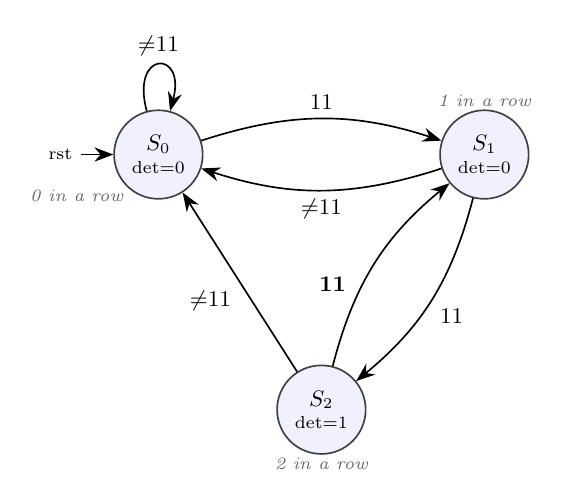
\begin{tikzpicture}[fsm,scale=0.90,transform shape]
\node[state,initial,label={[meaning]below left:{\textit{0 in a row}}}] (S0) at (0.00,0.00) {$S_{0}$\\[-2pt]{\scriptsize det=0}};
\node[state,label={[meaning]above:{\textit{1 in a row}}}] (S1) at (4.60,0.00) {$S_{1}$\\[-2pt]{\scriptsize det=0}};
\node[state,label={[meaning]below:{\textit{2 in a row}}}] (S2) at (2.30,-3.60) {$S_{2}$\\[-2pt]{\scriptsize det=1}};
\path (S0) edge[loop above] node[elab] {$\neq$11} (S0);
\path (S0) edge[bend left=18] node[elab] {11} (S1);
\path (S1) edge[bend left=18] node[elab] {$\neq$11} (S0);
\path (S1) edge[bend left=18] node[elab] {11} (S2);
\path (S2) edge[bend left=18] node[elab,pos=0.3] {\textbf{11}} (S1);
\path (S2) edge[] node[elab] {$\neq$11} (S0);
\end{tikzpicture}
\end{center}
{\small After a detection ($S_2$) another 11 is the \emph{first} of a new pair, so go to $S_1$, not $S_2$.
So ``11 11 11 11'' gives hits after the 2nd and 4th values only.}
\begin{center}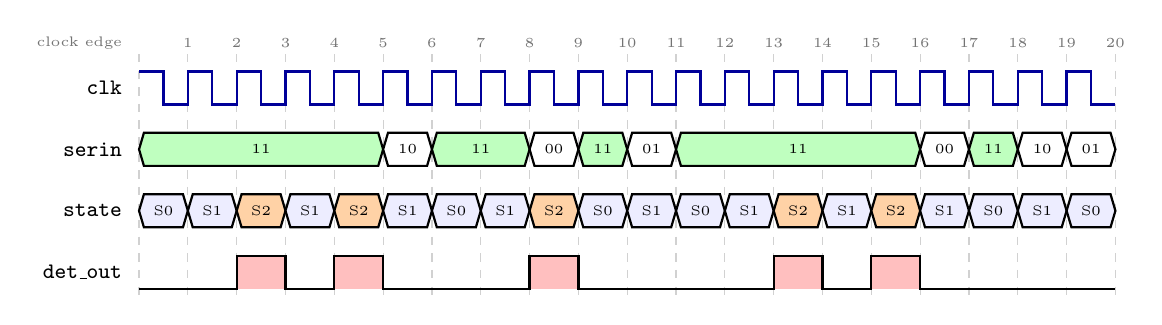
\begin{tikzpicture}[x=0.62cm,y=1cm,font=\scriptsize]
\draw[black!18,dashed] (0,0.64)--(0,-2.44);
\draw[black!18,dashed] (1,0.64)--(1,-2.44);
\node[black!55,font=\tiny] at (1,0.78) {1};
\draw[black!18,dashed] (2,0.64)--(2,-2.44);
\node[black!55,font=\tiny] at (2,0.78) {2};
\draw[black!18,dashed] (3,0.64)--(3,-2.44);
\node[black!55,font=\tiny] at (3,0.78) {3};
\draw[black!18,dashed] (4,0.64)--(4,-2.44);
\node[black!55,font=\tiny] at (4,0.78) {4};
\draw[black!18,dashed] (5,0.64)--(5,-2.44);
\node[black!55,font=\tiny] at (5,0.78) {5};
\draw[black!18,dashed] (6,0.64)--(6,-2.44);
\node[black!55,font=\tiny] at (6,0.78) {6};
\draw[black!18,dashed] (7,0.64)--(7,-2.44);
\node[black!55,font=\tiny] at (7,0.78) {7};
\draw[black!18,dashed] (8,0.64)--(8,-2.44);
\node[black!55,font=\tiny] at (8,0.78) {8};
\draw[black!18,dashed] (9,0.64)--(9,-2.44);
\node[black!55,font=\tiny] at (9,0.78) {9};
\draw[black!18,dashed] (10,0.64)--(10,-2.44);
\node[black!55,font=\tiny] at (10,0.78) {10};
\draw[black!18,dashed] (11,0.64)--(11,-2.44);
\node[black!55,font=\tiny] at (11,0.78) {11};
\draw[black!18,dashed] (12,0.64)--(12,-2.44);
\node[black!55,font=\tiny] at (12,0.78) {12};
\draw[black!18,dashed] (13,0.64)--(13,-2.44);
\node[black!55,font=\tiny] at (13,0.78) {13};
\draw[black!18,dashed] (14,0.64)--(14,-2.44);
\node[black!55,font=\tiny] at (14,0.78) {14};
\draw[black!18,dashed] (15,0.64)--(15,-2.44);
\node[black!55,font=\tiny] at (15,0.78) {15};
\draw[black!18,dashed] (16,0.64)--(16,-2.44);
\node[black!55,font=\tiny] at (16,0.78) {16};
\draw[black!18,dashed] (17,0.64)--(17,-2.44);
\node[black!55,font=\tiny] at (17,0.78) {17};
\draw[black!18,dashed] (18,0.64)--(18,-2.44);
\node[black!55,font=\tiny] at (18,0.78) {18};
\draw[black!18,dashed] (19,0.64)--(19,-2.44);
\node[black!55,font=\tiny] at (19,0.78) {19};
\draw[black!18,dashed] (20,0.64)--(20,-2.44);
\node[black!55,font=\tiny] at (20,0.78) {20};
\node[anchor=east,black!55,font=\tiny] at (-0.15,0.78) {clock edge};
\node[anchor=east,font=\footnotesize\ttfamily] at (-0.15,0.21) {clk};
\draw[thick,blue!60!black] (0.000,0.420) -- (0.500,0.420) -- (0.500,0.000) -- (1.000,0.000) -- (1.000,0.420) -- (1.500,0.420) -- (1.500,0.000) -- (2.000,0.000) -- (2.000,0.420) -- (2.500,0.420) -- (2.500,0.000) -- (3.000,0.000) -- (3.000,0.420) -- (3.500,0.420) -- (3.500,0.000) -- (4.000,0.000) -- (4.000,0.420) -- (4.500,0.420) -- (4.500,0.000) -- (5.000,0.000) -- (5.000,0.420) -- (5.500,0.420) -- (5.500,0.000) -- (6.000,0.000) -- (6.000,0.420) -- (6.500,0.420) -- (6.500,0.000) -- (7.000,0.000) -- (7.000,0.420) -- (7.500,0.420) -- (7.500,0.000) -- (8.000,0.000) -- (8.000,0.420) -- (8.500,0.420) -- (8.500,0.000) -- (9.000,0.000) -- (9.000,0.420) -- (9.500,0.420) -- (9.500,0.000) -- (10.000,0.000) -- (10.000,0.420) -- (10.500,0.420) -- (10.500,0.000) -- (11.000,0.000) -- (11.000,0.420) -- (11.500,0.420) -- (11.500,0.000) -- (12.000,0.000) -- (12.000,0.420) -- (12.500,0.420) -- (12.500,0.000) -- (13.000,0.000) -- (13.000,0.420) -- (13.500,0.420) -- (13.500,0.000) -- (14.000,0.000) -- (14.000,0.420) -- (14.500,0.420) -- (14.500,0.000) -- (15.000,0.000) -- (15.000,0.420) -- (15.500,0.420) -- (15.500,0.000) -- (16.000,0.000) -- (16.000,0.420) -- (16.500,0.420) -- (16.500,0.000) -- (17.000,0.000) -- (17.000,0.420) -- (17.500,0.420) -- (17.500,0.000) -- (18.000,0.000) -- (18.000,0.420) -- (18.500,0.420) -- (18.500,0.000) -- (19.000,0.000) -- (19.000,0.420) -- (19.500,0.420) -- (19.500,0.000) -- (20.000,0.000);
\node[anchor=east,font=\footnotesize\ttfamily] at (-0.15,-0.57) {serin};
\draw[thick,fill=green!25] (0.000,-0.570)--(0.100,-0.360)--(4.900,-0.360)--(5.000,-0.570)--(4.900,-0.780)--(0.100,-0.780)--cycle;
\node[font=\tiny] at (2.500,-0.570) {11};
\draw[thick,fill=white] (5.000,-0.570)--(5.100,-0.360)--(5.900,-0.360)--(6.000,-0.570)--(5.900,-0.780)--(5.100,-0.780)--cycle;
\node[font=\tiny] at (5.500,-0.570) {10};
\draw[thick,fill=green!25] (6.000,-0.570)--(6.100,-0.360)--(7.900,-0.360)--(8.000,-0.570)--(7.900,-0.780)--(6.100,-0.780)--cycle;
\node[font=\tiny] at (7.000,-0.570) {11};
\draw[thick,fill=white] (8.000,-0.570)--(8.100,-0.360)--(8.900,-0.360)--(9.000,-0.570)--(8.900,-0.780)--(8.100,-0.780)--cycle;
\node[font=\tiny] at (8.500,-0.570) {00};
\draw[thick,fill=green!25] (9.000,-0.570)--(9.100,-0.360)--(9.900,-0.360)--(10.000,-0.570)--(9.900,-0.780)--(9.100,-0.780)--cycle;
\node[font=\tiny] at (9.500,-0.570) {11};
\draw[thick,fill=white] (10.000,-0.570)--(10.100,-0.360)--(10.900,-0.360)--(11.000,-0.570)--(10.900,-0.780)--(10.100,-0.780)--cycle;
\node[font=\tiny] at (10.500,-0.570) {01};
\draw[thick,fill=green!25] (11.000,-0.570)--(11.100,-0.360)--(15.900,-0.360)--(16.000,-0.570)--(15.900,-0.780)--(11.100,-0.780)--cycle;
\node[font=\tiny] at (13.500,-0.570) {11};
\draw[thick,fill=white] (16.000,-0.570)--(16.100,-0.360)--(16.900,-0.360)--(17.000,-0.570)--(16.900,-0.780)--(16.100,-0.780)--cycle;
\node[font=\tiny] at (16.500,-0.570) {00};
\draw[thick,fill=green!25] (17.000,-0.570)--(17.100,-0.360)--(17.900,-0.360)--(18.000,-0.570)--(17.900,-0.780)--(17.100,-0.780)--cycle;
\node[font=\tiny] at (17.500,-0.570) {11};
\draw[thick,fill=white] (18.000,-0.570)--(18.100,-0.360)--(18.900,-0.360)--(19.000,-0.570)--(18.900,-0.780)--(18.100,-0.780)--cycle;
\node[font=\tiny] at (18.500,-0.570) {10};
\draw[thick,fill=white] (19.000,-0.570)--(19.100,-0.360)--(19.900,-0.360)--(20.000,-0.570)--(19.900,-0.780)--(19.100,-0.780)--cycle;
\node[font=\tiny] at (19.500,-0.570) {01};
\node[anchor=east,font=\footnotesize\ttfamily] at (-0.15,-1.35) {state};
\draw[thick,fill=blue!7] (0.000,-1.350)--(0.100,-1.140)--(0.900,-1.140)--(1.000,-1.350)--(0.900,-1.560)--(0.100,-1.560)--cycle;
\node[font=\tiny] at (0.500,-1.350) {S0};
\draw[thick,fill=blue!7] (1.000,-1.350)--(1.100,-1.140)--(1.900,-1.140)--(2.000,-1.350)--(1.900,-1.560)--(1.100,-1.560)--cycle;
\node[font=\tiny] at (1.500,-1.350) {S1};
\draw[thick,fill=orange!35] (2.000,-1.350)--(2.100,-1.140)--(2.900,-1.140)--(3.000,-1.350)--(2.900,-1.560)--(2.100,-1.560)--cycle;
\node[font=\tiny] at (2.500,-1.350) {S2};
\draw[thick,fill=blue!7] (3.000,-1.350)--(3.100,-1.140)--(3.900,-1.140)--(4.000,-1.350)--(3.900,-1.560)--(3.100,-1.560)--cycle;
\node[font=\tiny] at (3.500,-1.350) {S1};
\draw[thick,fill=orange!35] (4.000,-1.350)--(4.100,-1.140)--(4.900,-1.140)--(5.000,-1.350)--(4.900,-1.560)--(4.100,-1.560)--cycle;
\node[font=\tiny] at (4.500,-1.350) {S2};
\draw[thick,fill=blue!7] (5.000,-1.350)--(5.100,-1.140)--(5.900,-1.140)--(6.000,-1.350)--(5.900,-1.560)--(5.100,-1.560)--cycle;
\node[font=\tiny] at (5.500,-1.350) {S1};
\draw[thick,fill=blue!7] (6.000,-1.350)--(6.100,-1.140)--(6.900,-1.140)--(7.000,-1.350)--(6.900,-1.560)--(6.100,-1.560)--cycle;
\node[font=\tiny] at (6.500,-1.350) {S0};
\draw[thick,fill=blue!7] (7.000,-1.350)--(7.100,-1.140)--(7.900,-1.140)--(8.000,-1.350)--(7.900,-1.560)--(7.100,-1.560)--cycle;
\node[font=\tiny] at (7.500,-1.350) {S1};
\draw[thick,fill=orange!35] (8.000,-1.350)--(8.100,-1.140)--(8.900,-1.140)--(9.000,-1.350)--(8.900,-1.560)--(8.100,-1.560)--cycle;
\node[font=\tiny] at (8.500,-1.350) {S2};
\draw[thick,fill=blue!7] (9.000,-1.350)--(9.100,-1.140)--(9.900,-1.140)--(10.000,-1.350)--(9.900,-1.560)--(9.100,-1.560)--cycle;
\node[font=\tiny] at (9.500,-1.350) {S0};
\draw[thick,fill=blue!7] (10.000,-1.350)--(10.100,-1.140)--(10.900,-1.140)--(11.000,-1.350)--(10.900,-1.560)--(10.100,-1.560)--cycle;
\node[font=\tiny] at (10.500,-1.350) {S1};
\draw[thick,fill=blue!7] (11.000,-1.350)--(11.100,-1.140)--(11.900,-1.140)--(12.000,-1.350)--(11.900,-1.560)--(11.100,-1.560)--cycle;
\node[font=\tiny] at (11.500,-1.350) {S0};
\draw[thick,fill=blue!7] (12.000,-1.350)--(12.100,-1.140)--(12.900,-1.140)--(13.000,-1.350)--(12.900,-1.560)--(12.100,-1.560)--cycle;
\node[font=\tiny] at (12.500,-1.350) {S1};
\draw[thick,fill=orange!35] (13.000,-1.350)--(13.100,-1.140)--(13.900,-1.140)--(14.000,-1.350)--(13.900,-1.560)--(13.100,-1.560)--cycle;
\node[font=\tiny] at (13.500,-1.350) {S2};
\draw[thick,fill=blue!7] (14.000,-1.350)--(14.100,-1.140)--(14.900,-1.140)--(15.000,-1.350)--(14.900,-1.560)--(14.100,-1.560)--cycle;
\node[font=\tiny] at (14.500,-1.350) {S1};
\draw[thick,fill=orange!35] (15.000,-1.350)--(15.100,-1.140)--(15.900,-1.140)--(16.000,-1.350)--(15.900,-1.560)--(15.100,-1.560)--cycle;
\node[font=\tiny] at (15.500,-1.350) {S2};
\draw[thick,fill=blue!7] (16.000,-1.350)--(16.100,-1.140)--(16.900,-1.140)--(17.000,-1.350)--(16.900,-1.560)--(16.100,-1.560)--cycle;
\node[font=\tiny] at (16.500,-1.350) {S1};
\draw[thick,fill=blue!7] (17.000,-1.350)--(17.100,-1.140)--(17.900,-1.140)--(18.000,-1.350)--(17.900,-1.560)--(17.100,-1.560)--cycle;
\node[font=\tiny] at (17.500,-1.350) {S0};
\draw[thick,fill=blue!7] (18.000,-1.350)--(18.100,-1.140)--(18.900,-1.140)--(19.000,-1.350)--(18.900,-1.560)--(18.100,-1.560)--cycle;
\node[font=\tiny] at (18.500,-1.350) {S1};
\draw[thick,fill=blue!7] (19.000,-1.350)--(19.100,-1.140)--(19.900,-1.140)--(20.000,-1.350)--(19.900,-1.560)--(19.100,-1.560)--cycle;
\node[font=\tiny] at (19.500,-1.350) {S0};
\node[anchor=east,font=\footnotesize\ttfamily] at (-0.15,-2.13) {det\_out};
\fill[red!25] (2.000,-2.340) rectangle (3.000,-1.920);
\fill[red!25] (4.000,-2.340) rectangle (5.000,-1.920);
\fill[red!25] (8.000,-2.340) rectangle (9.000,-1.920);
\fill[red!25] (13.000,-2.340) rectangle (14.000,-1.920);
\fill[red!25] (15.000,-2.340) rectangle (16.000,-1.920);
\draw[thick,black] (0.000,-2.340) -- (1.000,-2.340) -- (1.000,-2.340) -- (2.000,-2.340) -- (2.000,-1.920) -- (3.000,-1.920) -- (3.000,-2.340) -- (4.000,-2.340) -- (4.000,-1.920) -- (5.000,-1.920) -- (5.000,-2.340) -- (6.000,-2.340) -- (6.000,-2.340) -- (7.000,-2.340) -- (7.000,-2.340) -- (8.000,-2.340) -- (8.000,-1.920) -- (9.000,-1.920) -- (9.000,-2.340) -- (10.000,-2.340) -- (10.000,-2.340) -- (11.000,-2.340) -- (11.000,-2.340) -- (12.000,-2.340) -- (12.000,-2.340) -- (13.000,-2.340) -- (13.000,-1.920) -- (14.000,-1.920) -- (14.000,-2.340) -- (15.000,-2.340) -- (15.000,-1.920) -- (16.000,-1.920) -- (16.000,-2.340) -- (17.000,-2.340) -- (17.000,-2.340) -- (18.000,-2.340) -- (18.000,-2.340) -- (19.000,-2.340) -- (19.000,-2.340) -- (20.000,-2.340);
\end{tikzpicture}\end{center}\begin{codeslice}{RTL -- 2-bit input, \texttt{11} on 2 consecutive clocks, non-overlapping}{det11x2.v}
\slicenote{This is the same counter-chain idea as Q1 with fewer states. Non-overlap means that after a hit, a new 11 counts as the first one again.}
\begin{lstlisting}
`timescale 1ns/1ps
// det_out = 1 when serin == 2'b11 on 2 consecutive clocks, NON-overlapping
module det11x2 (
    input  wire       clk,
    input  wire       rst,
    input  wire [1:0] serin,
    output reg        det_out
);
    localparam [1:0] S0 = 2'd0,   // 0 in a row
                     S1 = 2'd1,   // 1 in a row
                     S2 = 2'd2;   // 2 in a row -> det_out = 1
    reg [1:0] state, next_state;

    always @(posedge clk or posedge rst)
        if (rst) state <= S0;
        else     state <= next_state;

    always @(*) begin
        next_state = S0;
        if (serin == 2'b11)
            case (state)
                S0:      next_state = S1;
                S1:      next_state = S2;
                S2:      next_state = S1;   // non-overlap: count restarts at 1
                default: next_state = S0;   // (overlap would be: S2)
            endcase
    end

    always @(*) det_out = (state == S2);
endmodule
\end{lstlisting}
\end{codeslice}
{\small Testbench: copy \texttt{tb\_det01x3.v}, change the module name and compare against
\texttt{2'b11}. The repository has the RTL ready.}


\section{Predicted P6 -- serial number divisible by 3}
\begin{qbox}{Likely wording}
A binary number arrives serially, MSB first. Assert \texttt{div3} whenever the number received so far is
divisible by 3.
\end{qbox}
\begin{minipage}{0.45\textwidth}\centering
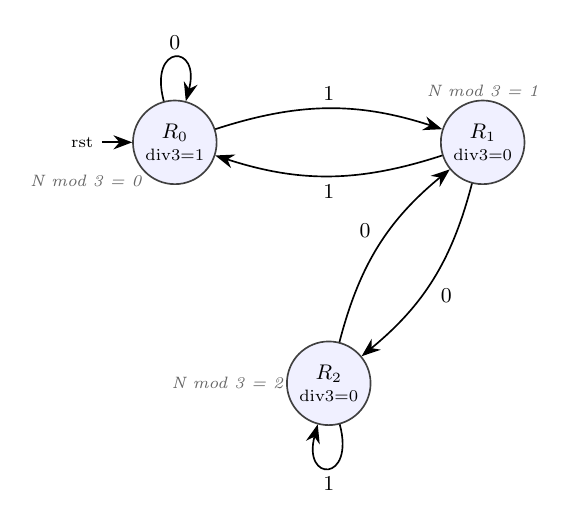
\begin{tikzpicture}[fsm,scale=0.85,transform shape]
\node[state,initial,label={[meaning]below left:{\textit{N mod 3 = 0}}}] (R0) at (0.00,0.00) {$R_{0}$\\[-2pt]{\scriptsize div3=1}};
\node[state,label={[meaning]above:{\textit{N mod 3 = 1}}}] (R1) at (4.60,0.00) {$R_{1}$\\[-2pt]{\scriptsize div3=0}};
\node[state,label={[meaning]left:{\textit{N mod 3 = 2}}}] (R2) at (2.30,-3.60) {$R_{2}$\\[-2pt]{\scriptsize div3=0}};
\path (R0) edge[loop above] node[elab] {0} (R0);
\path (R0) edge[bend left=18] node[elab] {1} (R1);
\path (R1) edge[bend left=18] node[elab] {1} (R0);
\path (R1) edge[bend left=18] node[elab] {0} (R2);
\path (R2) edge[bend left=18] node[elab] {0} (R1);
\path (R2) edge[loop below] node[elab] {1} (R2);
\end{tikzpicture}
\end{minipage}\hfill
\begin{minipage}{0.5\textwidth}\small
\begin{tabular}{c c c}
\toprule
$r$ & bin=0 ($2r$) & bin=1 ($2r+1$) \\ \midrule
0 & 0 & 1 \\ 1 & 2 & 0 \\ 2 & 1 & 2 \\ \bottomrule
\end{tabular}\\[4pt]
The state stores the remainder, not the number, so three states are enough
for any length. Generalise: divisible by $m$ needs $m$ states, next $=(2r+b)\bmod m$.
\end{minipage}
\begin{center}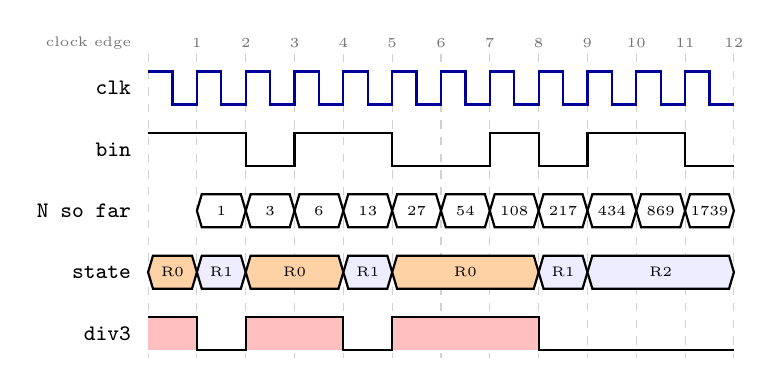
\begin{tikzpicture}[x=0.62cm,y=1cm,font=\scriptsize]
\draw[black!18,dashed] (0,0.64)--(0,-3.22);
\draw[black!18,dashed] (1,0.64)--(1,-3.22);
\node[black!55,font=\tiny] at (1,0.78) {1};
\draw[black!18,dashed] (2,0.64)--(2,-3.22);
\node[black!55,font=\tiny] at (2,0.78) {2};
\draw[black!18,dashed] (3,0.64)--(3,-3.22);
\node[black!55,font=\tiny] at (3,0.78) {3};
\draw[black!18,dashed] (4,0.64)--(4,-3.22);
\node[black!55,font=\tiny] at (4,0.78) {4};
\draw[black!18,dashed] (5,0.64)--(5,-3.22);
\node[black!55,font=\tiny] at (5,0.78) {5};
\draw[black!18,dashed] (6,0.64)--(6,-3.22);
\node[black!55,font=\tiny] at (6,0.78) {6};
\draw[black!18,dashed] (7,0.64)--(7,-3.22);
\node[black!55,font=\tiny] at (7,0.78) {7};
\draw[black!18,dashed] (8,0.64)--(8,-3.22);
\node[black!55,font=\tiny] at (8,0.78) {8};
\draw[black!18,dashed] (9,0.64)--(9,-3.22);
\node[black!55,font=\tiny] at (9,0.78) {9};
\draw[black!18,dashed] (10,0.64)--(10,-3.22);
\node[black!55,font=\tiny] at (10,0.78) {10};
\draw[black!18,dashed] (11,0.64)--(11,-3.22);
\node[black!55,font=\tiny] at (11,0.78) {11};
\draw[black!18,dashed] (12,0.64)--(12,-3.22);
\node[black!55,font=\tiny] at (12,0.78) {12};
\node[anchor=east,black!55,font=\tiny] at (-0.15,0.78) {clock edge};
\node[anchor=east,font=\footnotesize\ttfamily] at (-0.15,0.21) {clk};
\draw[thick,blue!60!black] (0.000,0.420) -- (0.500,0.420) -- (0.500,0.000) -- (1.000,0.000) -- (1.000,0.420) -- (1.500,0.420) -- (1.500,0.000) -- (2.000,0.000) -- (2.000,0.420) -- (2.500,0.420) -- (2.500,0.000) -- (3.000,0.000) -- (3.000,0.420) -- (3.500,0.420) -- (3.500,0.000) -- (4.000,0.000) -- (4.000,0.420) -- (4.500,0.420) -- (4.500,0.000) -- (5.000,0.000) -- (5.000,0.420) -- (5.500,0.420) -- (5.500,0.000) -- (6.000,0.000) -- (6.000,0.420) -- (6.500,0.420) -- (6.500,0.000) -- (7.000,0.000) -- (7.000,0.420) -- (7.500,0.420) -- (7.500,0.000) -- (8.000,0.000) -- (8.000,0.420) -- (8.500,0.420) -- (8.500,0.000) -- (9.000,0.000) -- (9.000,0.420) -- (9.500,0.420) -- (9.500,0.000) -- (10.000,0.000) -- (10.000,0.420) -- (10.500,0.420) -- (10.500,0.000) -- (11.000,0.000) -- (11.000,0.420) -- (11.500,0.420) -- (11.500,0.000) -- (12.000,0.000);
\node[anchor=east,font=\footnotesize\ttfamily] at (-0.15,-0.57) {bin};
\draw[thick,black] (0.000,-0.360) -- (1.000,-0.360) -- (1.000,-0.360) -- (2.000,-0.360) -- (2.000,-0.780) -- (3.000,-0.780) -- (3.000,-0.360) -- (4.000,-0.360) -- (4.000,-0.360) -- (5.000,-0.360) -- (5.000,-0.780) -- (6.000,-0.780) -- (6.000,-0.780) -- (7.000,-0.780) -- (7.000,-0.360) -- (8.000,-0.360) -- (8.000,-0.780) -- (9.000,-0.780) -- (9.000,-0.360) -- (10.000,-0.360) -- (10.000,-0.360) -- (11.000,-0.360) -- (11.000,-0.780) -- (12.000,-0.780);
\node[anchor=east,font=\footnotesize\ttfamily] at (-0.15,-1.35) {N so far};
\draw[thick,fill=white] (1.000,-1.350)--(1.100,-1.140)--(1.900,-1.140)--(2.000,-1.350)--(1.900,-1.560)--(1.100,-1.560)--cycle;
\node[font=\tiny] at (1.500,-1.350) {1};
\draw[thick,fill=white] (2.000,-1.350)--(2.100,-1.140)--(2.900,-1.140)--(3.000,-1.350)--(2.900,-1.560)--(2.100,-1.560)--cycle;
\node[font=\tiny] at (2.500,-1.350) {3};
\draw[thick,fill=white] (3.000,-1.350)--(3.100,-1.140)--(3.900,-1.140)--(4.000,-1.350)--(3.900,-1.560)--(3.100,-1.560)--cycle;
\node[font=\tiny] at (3.500,-1.350) {6};
\draw[thick,fill=white] (4.000,-1.350)--(4.100,-1.140)--(4.900,-1.140)--(5.000,-1.350)--(4.900,-1.560)--(4.100,-1.560)--cycle;
\node[font=\tiny] at (4.500,-1.350) {13};
\draw[thick,fill=white] (5.000,-1.350)--(5.100,-1.140)--(5.900,-1.140)--(6.000,-1.350)--(5.900,-1.560)--(5.100,-1.560)--cycle;
\node[font=\tiny] at (5.500,-1.350) {27};
\draw[thick,fill=white] (6.000,-1.350)--(6.100,-1.140)--(6.900,-1.140)--(7.000,-1.350)--(6.900,-1.560)--(6.100,-1.560)--cycle;
\node[font=\tiny] at (6.500,-1.350) {54};
\draw[thick,fill=white] (7.000,-1.350)--(7.100,-1.140)--(7.900,-1.140)--(8.000,-1.350)--(7.900,-1.560)--(7.100,-1.560)--cycle;
\node[font=\tiny] at (7.500,-1.350) {108};
\draw[thick,fill=white] (8.000,-1.350)--(8.100,-1.140)--(8.900,-1.140)--(9.000,-1.350)--(8.900,-1.560)--(8.100,-1.560)--cycle;
\node[font=\tiny] at (8.500,-1.350) {217};
\draw[thick,fill=white] (9.000,-1.350)--(9.100,-1.140)--(9.900,-1.140)--(10.000,-1.350)--(9.900,-1.560)--(9.100,-1.560)--cycle;
\node[font=\tiny] at (9.500,-1.350) {434};
\draw[thick,fill=white] (10.000,-1.350)--(10.100,-1.140)--(10.900,-1.140)--(11.000,-1.350)--(10.900,-1.560)--(10.100,-1.560)--cycle;
\node[font=\tiny] at (10.500,-1.350) {869};
\draw[thick,fill=white] (11.000,-1.350)--(11.100,-1.140)--(11.900,-1.140)--(12.000,-1.350)--(11.900,-1.560)--(11.100,-1.560)--cycle;
\node[font=\tiny] at (11.500,-1.350) {1739};
\node[anchor=east,font=\footnotesize\ttfamily] at (-0.15,-2.13) {state};
\draw[thick,fill=orange!35] (0.000,-2.130)--(0.100,-1.920)--(0.900,-1.920)--(1.000,-2.130)--(0.900,-2.340)--(0.100,-2.340)--cycle;
\node[font=\tiny] at (0.500,-2.130) {R0};
\draw[thick,fill=blue!7] (1.000,-2.130)--(1.100,-1.920)--(1.900,-1.920)--(2.000,-2.130)--(1.900,-2.340)--(1.100,-2.340)--cycle;
\node[font=\tiny] at (1.500,-2.130) {R1};
\draw[thick,fill=orange!35] (2.000,-2.130)--(2.100,-1.920)--(3.900,-1.920)--(4.000,-2.130)--(3.900,-2.340)--(2.100,-2.340)--cycle;
\node[font=\tiny] at (3.000,-2.130) {R0};
\draw[thick,fill=blue!7] (4.000,-2.130)--(4.100,-1.920)--(4.900,-1.920)--(5.000,-2.130)--(4.900,-2.340)--(4.100,-2.340)--cycle;
\node[font=\tiny] at (4.500,-2.130) {R1};
\draw[thick,fill=orange!35] (5.000,-2.130)--(5.100,-1.920)--(7.900,-1.920)--(8.000,-2.130)--(7.900,-2.340)--(5.100,-2.340)--cycle;
\node[font=\tiny] at (6.500,-2.130) {R0};
\draw[thick,fill=blue!7] (8.000,-2.130)--(8.100,-1.920)--(8.900,-1.920)--(9.000,-2.130)--(8.900,-2.340)--(8.100,-2.340)--cycle;
\node[font=\tiny] at (8.500,-2.130) {R1};
\draw[thick,fill=blue!7] (9.000,-2.130)--(9.100,-1.920)--(11.900,-1.920)--(12.000,-2.130)--(11.900,-2.340)--(9.100,-2.340)--cycle;
\node[font=\tiny] at (10.500,-2.130) {R2};
\node[anchor=east,font=\footnotesize\ttfamily] at (-0.15,-2.91) {div3};
\fill[red!25] (0.000,-3.120) rectangle (1.000,-2.700);
\fill[red!25] (2.000,-3.120) rectangle (3.000,-2.700);
\fill[red!25] (3.000,-3.120) rectangle (4.000,-2.700);
\fill[red!25] (5.000,-3.120) rectangle (6.000,-2.700);
\fill[red!25] (6.000,-3.120) rectangle (7.000,-2.700);
\fill[red!25] (7.000,-3.120) rectangle (8.000,-2.700);
\draw[thick,black] (0.000,-2.700) -- (1.000,-2.700) -- (1.000,-3.120) -- (2.000,-3.120) -- (2.000,-2.700) -- (3.000,-2.700) -- (3.000,-2.700) -- (4.000,-2.700) -- (4.000,-3.120) -- (5.000,-3.120) -- (5.000,-2.700) -- (6.000,-2.700) -- (6.000,-2.700) -- (7.000,-2.700) -- (7.000,-2.700) -- (8.000,-2.700) -- (8.000,-3.120) -- (9.000,-3.120) -- (9.000,-3.120) -- (10.000,-3.120) -- (10.000,-3.120) -- (11.000,-3.120) -- (11.000,-3.120) -- (12.000,-3.120);
\end{tikzpicture}\end{center}\begin{codeslice}{RTL -- remainder FSM (binary number arrives MSB first)}{div3\_fsm.v}
\slicenote{Shifting in bit $b$ turns $N$ into $2N+b$, so the next remainder is $(2r+b) \bmod 3$. Three states, one per remainder.}
\begin{lstlisting}
`timescale 1ns/1ps
// div3 = 1 when the binary number received so far (MSB first) is divisible by 3
module div3_fsm (
    input  wire clk,
    input  wire rst,
    input  wire bin,       // serial bit, MSB first
    output reg  div3
);
    localparam [1:0] R0 = 2'd0, R1 = 2'd1, R2 = 2'd2;   // remainder 0/1/2
    reg [1:0] state, next_state;

    always @(posedge clk or posedge rst)
        if (rst) state <= R0;
        else     state <= next_state;

    always @(*) begin
        case (state)                     // next = (2*r + bin) mod 3
            R0:      next_state = bin ? R1 : R0;
            R1:      next_state = bin ? R0 : R2;
            R2:      next_state = bin ? R2 : R1;
            default: next_state = R0;
        endcase
    end

    always @(*) div3 = (state == R0);
endmodule
\end{lstlisting}
\end{codeslice}


\section{Quick variations -- state tables you can draw in 2 minutes}
\begin{multicols}{2}\small
\textbf{``110'' non-overlapping, Mealy}\\
\begin{tabular}{c c c}\toprule
 & in=0 & in=1\\\midrule
$S_0$ & $S_0$/0 & $S_1$/0\\
$S_1$ (\texttt{1}) & $S_0$/0 & $S_2$/0\\
$S_2$ (\texttt{11}) & \cellcolor{orange!20}$S_0$/\textbf{1} & $S_2$/0\\\bottomrule
\end{tabular}\\[2pt]
{\footnotesize ``111'' still ends in ``11'' so stay in $S_2$.}

\medskip
\textbf{``1001'' overlapping, Mealy}\\
\begin{tabular}{c c c}\toprule
 & in=0 & in=1\\\midrule
$S_0$ & $S_0$/0 & $S_1$/0\\
$S_1$ (\texttt{1}) & $S_2$/0 & $S_1$/0\\
$S_2$ (\texttt{10}) & $S_3$/0 & $S_1$/0\\
$S_3$ (\texttt{100}) & $S_0$/0 & \cellcolor{orange!20}$S_1$/\textbf{1}\\\bottomrule
\end{tabular}\\[2pt]
{\footnotesize After ``1001'' the last 1 is reused, so go to $S_1$.}

\medskip
\textbf{Three consecutive 1s (``111''), overlapping, Moore}\\
\begin{tabular}{c c c c}\toprule
 & in=0 & in=1 & out\\\midrule
$S_0$ & $S_0$ & $S_1$ & 0\\
$S_1$ & $S_0$ & $S_2$ & 0\\
$S_2$ & $S_0$ & $S_3$ & 0\\
$S_3$ & $S_0$ & $S_3$ & \textbf{1}\\\bottomrule
\end{tabular}

\columnbreak
\textbf{``0110'' overlapping, Moore}\\
\begin{tabular}{c c c c}\toprule
 & in=0 & in=1 & out\\\midrule
$S_0$ & $S_1$ & $S_0$ & 0\\
$S_1$ (\texttt{0}) & $S_1$ & $S_2$ & 0\\
$S_2$ (\texttt{01}) & $S_1$ & $S_3$ & 0\\
$S_3$ (\texttt{011}) & $S_4$ & $S_0$ & 0\\
$S_4$ (\texttt{0110}) & $S_1$ & $S_2$ & \textbf{1}\\\bottomrule
\end{tabular}\\[2pt]
{\footnotesize From $S_4$: ``01100'' ends in ``0'', and ``01101'' ends in ``01''.}

\medskip
\textbf{Even number of 1s (parity), Moore}\\
\begin{tabular}{c c c c}\toprule
 & in=0 & in=1 & out\\\midrule
EVEN & EVEN & ODD & 1\\
ODD & ODD & EVEN & 0\\\bottomrule
\end{tabular}

\medskip
\textbf{Converting Moore $\to$ Mealy}: move each state's output onto every arrow
\emph{entering} it, then merge states that now behave identically (``010'': 4 $\to$ 3 states).\\[2pt]
\textbf{Mealy $\to$ Moore}: split any state that is entered with different outputs.
\end{multicols}

\begin{tip}[Likely short (theory) questions]
\begin{enumerate}[leftmargin=*,itemsep=0pt]
\item Differentiate Moore and Mealy FSMs. Which one needs more states, and which responds faster?
\item What is the difference between overlapping and non-overlapping detection? Show it with a waveform.
\item Why are FSMs coded with separate sequential and combinational always blocks?
\item What causes an unintended latch in an FSM, and how do you avoid it?
\item Binary vs.\ one-hot vs.\ Gray state encoding: how many flip-flops does each need for $N$ states?
  (binary $\lceil\log_2 N\rceil$, one-hot $N$, Gray $\lceil\log_2 N\rceil$.)
\item Why does the testbench change inputs on the negative edge or after a small delay, and not at
  \texttt{posedge}?
\item Synchronous vs.\ asynchronous reset: write both forms of the state register.
\end{enumerate}
\end{tip}

\begin{codeslice}{Synchronous vs.\ asynchronous reset}{snippet}
\begin{lstlisting}
always @(posedge clk or posedge rst)   // ASYNC: reset acts immediately
    if (rst) state <= S0; else state <= next_state;

always @(posedge clk)                  // SYNC: reset only at a clock edge
    if (rst) state <= S0; else state <= next_state;
\end{lstlisting}
\end{codeslice}

\section*{Running the code}
{\small
\texttt{iverilog -o sim rtl/seq010\_moore.v tb/tb\_seq010.v \&\& vvp sim \&\& gtkwave tb\_seq010.vcd}\\
The same works for every \texttt{rtl/*.v} + \texttt{tb/tb\_*.v} pair. Signals to add in GTKWave:
\texttt{clk, rst, serin, dut.state, det\_out}.}

\end{document}
